%!TEX TS-program = xelatex
% https://habr.com/ru/post/144648/
\documentclass[a4paper,14pt,ukrainian]{extreport}
\usepackage{xltxtra}

\usepackage{extsizes}
%\usepackage{cmap} % для кодировки шрифтов в pdf
\usepackage{fontspec}
\defaultfontfeatures{Ligatures={TeX}} 
\setmainfont[Ligatures=TeX]{Times New Roman}
\setmonofont[Mapping=tex-text]{Courier New}
\usepackage[ukrainian]{babel}

\usepackage{graphicx} % для вставки картинок
\usepackage{amssymb,amsfonts,amsmath,amsthm} % математические дополнения от АМС
\usepackage{indentfirst} % отделять первую строку раздела абзацным отступом тоже
\usepackage[usenames,dvipsnames]{color} % названия цветов
\usepackage{makecell}
\usepackage{multirow} % улучшенное форматирование таблиц
\usepackage{ulem} % подчеркивания

\usepackage{tikz}
\usepackage{pgfplots}
\pgfplotsset{compat=1.17}
\usepackage[europeanresistors, RPvoltages]{circuitikz}
\usetikzlibrary{arrows,decorations.markings}

\usepackage[nodisplayskipstretch]{setspace}
\onehalfspacing % полуторный интервал
\frenchspacing

\usepackage{fancyhdr}
\pagestyle{fancy}
\fancyhf{}
\fancyhead[R]{\thepage}
\fancyheadoffset{0mm}
\fancyfootoffset{0mm}
\setlength{\headheight}{17pt}
\renewcommand{\headrulewidth}{0pt}
\renewcommand{\footrulewidth}{0pt}
\fancypagestyle{plain}{ 
    \fancyhf{}
    \rhead{\thepage}}
\setcounter{page}{1} 

\usepackage[tableposition=top]{caption}
\usepackage{subcaption}
\DeclareCaptionLabelFormat{gostfigure}{Рисунок #2}
\DeclareCaptionLabelFormat{gosttable}{Табл. #2}
\DeclareCaptionLabelSeparator{gost}{~--~}
\captionsetup{labelsep=gost}
\captionsetup[figure]{labelformat=gostfigure}
\captionsetup[table]{labelformat=gosttable}
\renewcommand{\thesubfigure}{\asbuk{subfigure}}

\usepackage{titlesec}
 
\titleformat{\chapter}[display]
    {\filcenter}
    {\bfseries\texorpdfstring{\MakeUppercase{\chaptertitlename}}{{\chaptertitlename}} \thechapter}
    {4pt}
    {\bfseries\MakeUppercase}{}
 
\titleformat{\section}
    {\normalsize\bfseries}
    {\thesection.}
    {1em}{}
 
\titleformat{\subsection}
    {\normalsize\bfseries}
    {\thesubsection.}
    {1em}{}

% Настройка вертикальных и горизонтальных отступов
\titlespacing*{\chapter}{0pt}{-30pt}{4pt}
\titlespacing*{\section}{\parindent}{*2}{*1}
\titlespacing*{\subsection}{\parindent}{*2}{*1}

\usepackage{geometry}
% \geometry{left=3cm}
% \geometry{right=1.5cm}
% \geometry{top=2.4cm}
% \geometry{bottom=2.4cm}
\geometry{left=2cm}
\geometry{right=1cm}
\geometry{top=2cm}
\geometry{bottom=2cm}

\usepackage{enumitem}
\makeatletter
    \AddEnumerateCounter{\asbuk}{\@asbuk}{м)}
\makeatother
\setlist{nolistsep}
%\renewcommand{\labelitemi}{-}
%\renewcommand{\labelenumi}{\asbuk{enumi})}
%\renewcommand{\labelenumii}{\arabic{enumii})}

\usepackage{tocloft}
\renewcommand{\cfttoctitlefont}{\hspace{0.38\textwidth} \bfseries\texorpdfstring{\MakeUppercase}{}}
\renewcommand{\cftbeforetoctitleskip}{-0.5em}
%\renewcommand{\cftaftertoctitle}{\mbox{}\hfill \\ \mbox{}\hfill{\footnotesize Стр.}\vspace{-2.5em}}
\renewcommand{\cftchapfont}{\normalsize \texorpdfstring{\MakeUppercase{\chaptername}}{{\chaptername}} }
\renewcommand\cftchappagefont{\mdseries}
\renewcommand{\cftsecfont}{\hspace{-11pt}}
\renewcommand{\cftsubsecfont}{\hspace{11pt}}
\renewcommand{\cftbeforechapskip}{1em}
\renewcommand{\cftparskip}{-1mm}
\renewcommand{\cftdotsep}{1}
\renewcommand{\cftchapleader}{\cftdotfill{\cftdotsep}}
\renewcommand{\cftsecaftersnum}{.}
\setcounter{tocdepth}{2} % задать глубину оглавления — до subsection включительно

\newcommand{\likechapterheading}[1]{ 
    \begin{center}
    \textbf{\texorpdfstring{\MakeUppercase{#1}}{{#1}}}
    \end{center}}

\makeatletter
    \newcommand{\l@likechapter}[2]{{\bfseries\@dottedtocline{0}{0pt}{0pt}{#1}{#2}}}
\makeatother
\newcommand{\likechapter}[1]{    
    \likechapterheading{#1}
    \phantomsection    
    \addcontentsline{toc}{likechapter}{\texorpdfstring{\MakeUppercase{#1}}{{#1}}}}

\usepackage[square,numbers,sort&compress]{natbib}
\renewcommand{\bibnumfmt}[1]{#1.\hfill} % нумерация источников в самом списке — через точку
\renewcommand{\bibsection}{\likechapter{Список використаної літератури}} % заголовок специального раздела
\setlength{\bibsep}{0pt}

\usepackage[hidelinks]{hyperref}
\usepackage{microtype}

\usepackage{listings}

\lstdefinestyle{code}{
    basicstyle=\ttfamily\footnotesize,
    breakatwhitespace=false,         
    breaklines=true,                 
    captionpos=b,                    
    keepspaces=true,                            
    numbersep=1pt,                  
    showspaces=false,                
    showstringspaces=false,
    showtabs=false,                  
    tabsize=2
}

\newcommand{\inlinecode}[1]{\texttt{\small #1}}

\usepackage{float}

\newcommand{\append}[1]{
    \phantomsection
    \addcontentsline{toc}{section}{#1}
    \begin{center}
        \textbf{#1}
    \end{center}
}

\begin{document}
\begin{titlepage}
    \thispagestyle{empty}
    \begin{center}
        Міністерство освіти і науки України\\
        Національний технічний університет України\\
        <<Київський політехнічний інститут ім. І. Сікорського>>\\
        Інститут прикладного системного аналізу
    \end{center}
    \vspace{50mm}
    \begin{center}
        \textbf{Курсова робота} \\
        з дисципліни \\
        <<Теорія керування>>
    \end{center}
    \vspace{30mm}
    \begin{flushright}
        \textbf{Виконав}: студент 4 курсу \\
        групи КА-81 \\
        Галганов Олексій \\
        \textbf{Прийняв}: професор \\
        Романенко Віктор Демидович
    \end{flushright}
    \vspace{40mm}
    \begin{center}
        \textbf{Київ 2021}
    \end{center}
\end{titlepage}
\microtypesetup{protrusion=false}
\tableofcontents
\microtypesetup{protrusion=true}
    % !TEX root = ../main.tex
\newpage
\chapter{Вступ}
\section{Теоретичні дані}
Розглядається одноконтурна система автоматичного цифрового керування (ЦК) з наступною структурною схемою:
\begin{figure}[!ht]
    \begin{circuitikz}[scale = 0.9, transform shape]
        \draw (0, 0) to[switch] (2, 0) node[above left = 0.3em]{$G(s)$} 
        to[lamp] (3, 0) to[switch] (5, 0) node[above left = 0.3em]{$E^*(s)$};
        \node[draw, minimum width = 2cm, minimum height = 1cm, anchor = south west] at (5, -0.5){$W_P^*(s)$};
        \draw (7, 0) to[switch] (9, 0) node[above left = 0.3em]{$u^*(s)$} (9, 0); 
        \node[draw, minimum width = 2cm, minimum height = 1cm, anchor = south west] at (9, -0.5){$W_E^*(s)$};
        \draw (11, 0) to (13, 0);
        \node at (12, 0.6) {$u(s)$};
        \node[draw, minimum width = 2cm, minimum height = 1cm, anchor = south west] at (13,-0.5){$W_O^*(s)$};
        \draw[decoration={markings,mark=at position 1 with
            {\arrow[scale=2,>=stealth]{>}}},postaction={decorate}] (15, 0) -- (17, 0);
        \draw[decoration={markings,mark=at position 1 with
            {\arrow[scale=2,>=stealth]{>}}},postaction={decorate}] (1.5, 0) -- (2.07, 0);
        \draw[decoration={markings,mark=at position 1 with
            {\arrow[scale=2,>=stealth]{>}}},postaction={decorate}] (4.5, 0) -- (5, 0);
        \draw[decoration={markings,mark=at position 1 with
            {\arrow[scale=2,>=stealth]{>}}},postaction={decorate}] (8.5, 0) -- (9, 0);
        \draw[decoration={markings,mark=at position 1 with
            {\arrow[scale=2,>=stealth]{>}}},postaction={decorate}] (12.5, 0) -- (13, 0);
        \draw[decoration={markings,mark=at position 1 with
            {\arrow[scale=2,>=stealth]{>}}},postaction={decorate}] (2.5, -2) -- (2.5, -0.4);
        \draw (2.5, -2) -- (10, -2);
        \draw (10, -2) to[switch] (12, -2) node[above left = 0.3em]{$y^*(s)$}; 
        \node [above = 0.3em] at (16, 0) {$y(s)$};
        \draw (12, -2) -- (16, -2) -- (16, 0);
        \node at (1.7, -0.4) {$+$};
        \node at (2.8, -0.8) {$-$};
        \draw [fill, radius=0.15em] (16, 0) circle;
    \end{circuitikz}
    \caption{Структурна схема типового контура ЦК}
    \label{pic1}
\end{figure}

Тут $W_O(s)$ -- передаточна функція об'єкта керування по керуючому діянню, $G(s)$ і $u(s)$ -- відповідно задаюче і керуюче діяння в формі
перетворення Лапласа, $W_p^*(s)$ -- передаточна функція цифрового регулятора (ЦАП) у формі дискретного перетворення Лапласа,
$W_E(s)$ -- передаточна функція цифро-аналогового регулятора, $E^*(s)$, $u^*(s)$, $y^*(s)$ -- відповідно помилка керування,
керуюче діяння та вихідна керована координата у формі дискретного перетворення Лапласа. Передаточні функції об'єкта для окремих задач мають вигляд
\begin{gather}\label{W_0}
    W_O(s) = \frac{
        k e^{-\tau s}
    }{
        (T_1 s + 1) (T_2 s + 1) (T_3 s + 1)
    } \\
    \label{W_0_12}
    W_O(s) = \frac{
        k (T_1 s + 1)
    }{
        (T_2 s + 1) (T_3 s + 1)
    }
\end{gather}
де $k$ -- коефіцієнт передачі об'єкта керування, $T_1$, $T_2$, $T_3$ -- сталі часу в секундах, $\tau$ -- час запізнення в секундах.

Регулятор ЦК, представлений в різницевій формі на основі позиційного алгоритма пропорційно-інтегрально-диференціального (ПІД)
закону керування записується таким чином:
\begin{gather}\label{PID}
    u(n T_0) = K_p \left(
        e(n T_0) + \frac{T_0}{T_I} \sum_{i=1}^n e(i T_0) +
        \frac{T_D}{T_0} \left[e(n T_0) - e((n-1)T_0)\right]
    \right)
\end{gather}
Тут $u(n T_0)$ та $e(n T_0)$ -- відповідно керуюче діяння і помилка керування в $n$-тий період квантування,
$K_p$ -- коефіцієнт передачі регулятора, $T_I$ та $T_D$ -- відповідно сталі часу інтегрування та диференціювання в секундах,
$T_0$ -- період квантування в секундах. 

Відповідно до \eqref{PID}, дискретна передаточна функція ПІД-регулятора має вигляд
\begin{gather}
    W_p(z) = K_p \left(
        1 + \frac{T_0}{T_I \left(1 - z^{-1}\right)} + \frac{T_D\left(1 - z^{-1}\right)}{T_0}
    \right)
\end{gather}
Якщо час диференціювання $T_D = 0$, то для цифрового ПІ-регулятора матимемо дискретну передаточну функцію
\begin{gather}\label{PI}
    W_p(z) = K_p \left(
        1 + \frac{T_0}{T_I \left(1 - z^{-1}\right)}
    \right)
\end{gather}
де $z = e^{sT_0}$ -- оператор $z$-перетворення.

\section{Завдання курсової роботи}
\begin{enumerate}
    \item Розрахувати дискретну передаточну функцію замкненого контура 
        цифрового керування, попередньо розрахувавши дискретну передаточну 
        функцію приведеної неперервної частини (ПНЧ) об'єкта
        \begin{gather}
            W_\text{п}(z) = z \left\{W_E(s) \cdot W_O(s) \right\}
        \end{gather} 
        для наступних варіантів передаточної функції об'єкта:
        $W_O(S) = \frac{k}{T_1 s + 1}$, $W_O(S) = \frac{k}{(T_1 s + 1)(T_2 s + 1)}$, 
        $W_O(S) = \frac{k e^{-\tau s}}{T_1 s + 1}$, $W_O(S) = \frac{k e^{-\tau s}}{(T_1 s + 1)(T_2 s + 1)}$.
    \item Розрахувати періоди квантування в системі цифрового керування для об'єктів
        \begin{gather}\label{W_01}
            W_{O_1}(s) = \frac{k e^{-\tau s}}{T_1 s + 1} \\
            \label{W_02}
            W_{O_2}(s) = \frac{k e^{-\tau s}}{(T_1 s + 1)(T_2 s + 1)}
        \end{gather}
        і для об'єкта \eqref{W_0_12}, передаточна функція якого має динаміку в чисельнику.
    \item На основі методу <<прямого>> синтезу визначити структуру і оптимальні настройки регуляторів цифрового керування і неперервного
        регулятора для управління об'єктами, передаточні функції яких мають вигляд \eqref{W_01}, \eqref{W_02}. 
        При цьому приймається період квантування $T_0$, розрахований у пункті 2 на основі умови забезпечення необхідної точності керування.
        Значення коефіцієнта підсилення регулятора
        $K_{P_\text{опт}}$ необхідно визначити при таких параметрах настройки $\lambda$:

        a) $\lambda = \frac{1}{T_1}$; б) $\lambda = \frac{1}{1.5 T_1}$; в) $\lambda = \frac{1}{2T_1}$; г) $\lambda = \frac{1}{3T_1}$.

        Для вказаного набору параметрів настройки $\lambda$ шляхом цифрового моделювання побудувати перехідні процеси в замкненому контурі цифрового керування.
    \item  Розрахувати оптимальні параметри ПІ-регулятора цифрового керування і 
        періоду квантування резонансним методом для об'єкта керування \eqref{W_0}, \eqref{W_02}. На основі цифрового моделювання побудувати перехідні процеси 
        вихідної координати $y$ в замкненому контурі при подачі імпульсних тестів 
        на задаюче діяння цифрового регулятора. 
    \item Виконати синтез лінійно-квадратичного регулятора стану і виконати 
        цифрове моделювання замкненої системи з регулятором стану. 
    \item Дослідити стійкість контура цифрового керування, розрахованої за 
        пунктом 3. При цьому використовувати відомі критерії стійкості. 
    \item Сформувати позиційний і швидкісний алгоритм цифрового керування в формі, зручній для програмування для регуляторів цифрового керування відповідно до пунктів 3, 4.
\end{enumerate}

\section{Значення коефіцієнтів та сталих}
\begin{center}
    \begin{tabular}{|c|c|c|c|c|}
        \hline
        $k$ & $T_1$ & $T_2$ & $T_3$ & $\tau$ \\
        \hline
        9.32 & 35 & 19 & 11 & 14 \\ 
        \hline
    \end{tabular}
\end{center}
$k$ -- коефіцієнт передачі об'єкта керування, $T_1$, $T_2$, $T_3$ -- сталі часу в секундах, $\tau$ -- час запізнення в секундах.
    \newpage
    % !TEX root = ../main.tex
\chapter{Розрахунок дискретних передаточних функцій}
\section{Теоретичні дані}
% Відповідно до рисунку \ref{pic1}, керовану координату $y(s)$
% можна записати як 
% \begin{gather}\label{eq:2_1}
%     y(s) = W_{n}(s) \cdot u^* (s)
% \end{gather}, де
% $u^*(s)$ -- дискретне перетворення Лапласа керуючого діяння $u(t)$,
% яке дорівнює
% \begin{gather}
%     u^*(s) = W_p^*(s) \cdot E^*(s)
% \end{gather}
% а $W_n(s) = W_E(s) \cdot W_O(S)$ -- передаточна функція приведеної неперервної частини.
% При цьому
% \begin{gather}
%     E^*(s) = G^*(s) - y^*(s) 
% \end{gather}
% де $E^*(s)$, $G^*(s)$, $y^*(s)$ --- відповідно дискретне перетворення Лапласа від
% помилки керування, задаючого діяння і керованої координати.

% Застосуємо до \eqref{eq:2_1} дискретне перетворення Лапласа:
% \begin{gather}
%     y^*(s) = W_{n}^*(s) \cdot u^*(s)
% \end{gather}
% Після

Дискретну передаточну функцію приведеної неперервної частини (ПНЧ)
об'єкта має вигляд
\begin{gather}
    \nonumber
    W_{\text{п}}(z) = z \left\{W_E(s) \cdot W_O(s) \right\} = 
    z\left\{ \frac{1-e^{-s T_0}}{s} \cdot W_O(S)\right\} = \\ =
    z\left\{\left(1 - e^{-s T_0}\right)\cdot \frac{W_O(s)}{s}\right\} = 
    \left(1 - z^{-1}\right) \cdot z\left\{\frac{W_O(s)}{s} \right\}
\end{gather}
Дискретна передаточна функція замкненого контуру цифрового керування має вигляд
\begin{gather}
    W_{\text{з}}(z) = \frac{
        W_{\text{п}}(z) \cdot W_p(z)
    }{1 + W_{\text{п}}(z) \cdot W_p(z)}
\end{gather}
де $W_p(z)$ -- дискретна передаточна функція регулятора, що для ПІД-регулятора
має вигляд \eqref{PID}, а для ПІ-регулятора -- вигляд \eqref{PI}.
Далі за текстом термін <<дискретна передаточна функція>> буде скорочено до ДПФ.

\section{Випадок \texorpdfstring{$W_O(S) = \frac{k}{T_1 s + 1}$}{1}}
Обчислимо $z$-перетворення для $\frac{W_O(S)}{s} = \frac{k}{s(T_1 s + 1)} = \frac{k}{s} - \frac{k T_1}{T_1 s + 1}$.
За таблицею $z$-перетворення отримаємо
\begin{gather}
    z\left\{\frac{W_O(s)}{s} \right\} = 
    \frac{kz}{z-1} - \frac{kz}{z - e^{T_0 / T_1}} = 
    \frac{k \left(1 - e^{- T_0 / T_1}\right)z}{
        (z-1) \left(z - e^{- T_0 / T_1}\right)
    }
\end{gather}
Тому ДПФ ПНЧ має вигляд
\begin{gather}
    W_{\text{п}}(z) = \left(1 - z^{-1}\right) \cdot z\left\{\frac{W_O(s)}{s} \right\} = 
    \frac{z-1}{z} \cdot \frac{k \left(1 - e^{- T_0 / T_1}\right)z}{
        (z-1) \left(z - e^{- T_0 / T_1}\right)
    } = \nonumber \\ =
    \frac{k \left(1 - e^{- T_0 / T_1}\right)}{
        z - e^{- T_0 / T_1}
    }
\end{gather}
Отже, ДПФ замкненого контуру цифрового керування з ПІД-регулятором має вигляд
\begin{gather}
    W_{\text{з}}(z) = \frac{
        W_{\text{п}} (z) \cdot W_p(z)
    }{1 + W_{\text{п}} (z) \cdot W_p(z)} = 
    \frac{
        \frac{k \left(1 - e^{- T_0 / T_1}\right)}{
            z - e^{- T_0 / T_1}
        } \cdot K_p \left(
            1 + \frac{T_0}{T_I \left(1 - z^{-1}\right)} + \frac{T_D\left(1 - z^{-1}\right)}{T_0}
        \right)
    }{
        1 + 
        \frac{k \left(1 - e^{- T_0 / T_1}\right)}{
            z - e^{- T_0 / T_1}
        } \cdot K_p \left(
            1 + \frac{T_0}{T_I \left(1 - z^{-1}\right)} + \frac{T_D\left(1 - z^{-1}\right)}{T_0}
        \right)
    } = \nonumber \\ =
    \frac{
        k \left(1 - e^{- T_0 / T_1}\right) \cdot K_p \left(
            1 + \frac{T_0}{T_I \left(1 - z^{-1}\right)} + \frac{T_D\left(1 - z^{-1}\right)}{T_0}
        \right)
    }{
        \left(z - e^{- T_0 / T_1}\right) + k \left(1 - e^{- T_0 / T_1}\right) \cdot K_p \left(
            1 + \frac{T_0}{T_I \left(1 - z^{-1}\right)} + \frac{T_D\left(1 - z^{-1}\right)}{T_0}
        \right)
    } = \nonumber \\ =
    \mbox{\normalsize $\frac{
        k K_p \left(1 - e^{- T_0 / T_1}\right)
        \left(
            T_0 T_I \left(1 - z^{-1}\right) + T_0^2 + T_I T_D \left(1 - z^{-1}\right)^2
        \right)
    }{
        \left(z - e^{- T_0 / T_1}\right) T_0 T_I \left(1 - z^{-1}\right) + k K_p \left(1 - e^{- T_0 / T_1}\right)
        \left(
            T_0 T_I \left(1 - z^{-1}\right) + T_0^2 + T_I T_D \left(1 - z^{-1}\right)^2
        \right) 
    }$} = \nonumber \\ =
    \mbox{\normalsize $\frac{
        k K_p \left(1 - e^{- T_0 / T_1}\right)
        \left(
            T_0 T_I \left(1 - z^{-1}\right) + T_0^2 + T_I T_D \left(1 - z^{-1}\right)^2
        \right) z^{-1}
    }{
        \left(1 - e^{- T_0 / T_1} z^{-1}\right) T_0 T_I \left(1 - z^{-1}\right) + k K_p \left(1 - e^{- T_0 / T_1}\right)
        \left(
            T_0 T_I \left(1 - z^{-1}\right) + T_0^2 + T_I T_D \left(1 - z^{-1}\right)^2
        \right) z^{-1}
    }$}
    % = \nonumber \\ =
    % \mbox{\normalsize $\frac{
    %     k K_p \left(z - e^{- T_0 / T_1}\right)
    %     \left(
    %         T_0 T_I  z \left(z - 1\right) + z^2 T_0^2 + T_I T_D \left(z - 1\right)^2
    %     \right)
    % }{
    %     \left(z - e^{- T_0 / T_1}\right) T_0 T_I z \left(z - 1\right) + k K_p \left(z - e^{- T_0 / T_1}\right)
    %     \left(
    %         T_0 T_I z \left(z - 1\right) + z^2 T_0^2 + T_I T_D \left(z - 1\right)^2
    %     \right)
    % }$}
\end{gather}
Відповідно, з ПІ-регулятором ($T_D = 0$):
\begin{gather}
    W_{\text{з}}(z) = \mbox{\normalsize $\frac{
        k K_p \left(1 - e^{- T_0 / T_1}\right)
        \left(
            T_0 T_1 \left(1 - z^{-1}\right) + T_0^2
        \right) z^{-1}
    }{
        \left(1 - e^{- T_0 / T_1} z^{-1}\right) T_0 T_1 \left(1 - z^{-1}\right) + k K_p \left(1 - e^{- T_0 / T_1}\right)
        \left(
            T_0 T_1 \left(1 - z^{-1}\right) + T_0^2
        \right) z^{-1}
    }$} = \nonumber \\ =
    \frac{
        k K_p \left(z - e^{- T_0 / T_1}\right)
        \left(
            T_1 \left(1 - z^{-1}\right) + T_0
        \right) z^{-1}
    }{
        \left(1 - e^{- T_0 / T_1 z^{-1}}\right) T_1 \left(1 - z^{-1}\right) + k K_p \left(z - e^{- T_0 / T_1}\right)
        \left(
            T_1 \left(1 - z^{-1}\right) + T_0
        \right) z^{-1}
    }
\end{gather}

\section{Випадок \texorpdfstring{$W_O(S) = \frac{k}{(T_1 s + 1)(T_2 s + 1)}$}{2}}
Обчислимо $z$-перетворення для $\frac{W_O(S)}{s} = \frac{k}{s(T_1 s + 1)(T_2 s + 1)} = 
\frac{k}{s} - \frac{k T_1^2}{(T_1 - T_2) (T_1 s + 1)} + \frac{k T_2^2}{(T_1 - T_2) (T_2 s + 1)}$.
За таблицею $z$-перетворення отримаємо
\begin{gather}
    z\left\{\frac{W_O(s)}{s} \right\} = 
    k \left(
        \frac{z}{z-1} - \frac{az}{T_1 (z - d_1)} +
        \frac{bz}{T_2 (z - d_2)}
    \right)
\end{gather}
де $a = \frac{T_1^2}{T_1 - T_2}$, $b = \frac{T_2^2}{T_1 - T_2}$,
$d_1 = e^{-T_0 / T_1}$, $d_2 = e^{-T_0 / T_2}$.
Тому ДПФ ПНЧ має вигляд
\begin{gather}
    W_{\text{п}}(z) = \left(1 - z^{-1}\right) \cdot z\left\{\frac{W_O(s)}{s} \right\} = 
    \nonumber \\ =
    \frac{z-1}{z} \cdot k \left(
        \frac{z}{z-1} - \frac{az}{T_1 (z - d_1)} +
        \frac{bz}{T_2 (z - d_2)}
    \right) = \nonumber \\ =
    k \left(
        1 - \frac{a(z-1)}{T_1 (z - d_1)} +
        \frac{b(z-1)}{T_2 (z - d_2)}
    \right)
\end{gather}
Отже, ДПФ замкненого контуру цифрового керування з ПІД-регулятором має вигляд
\begin{gather}
    W_{\text{з}}(z) = \frac{
        W_{\text{п}} (z) \cdot W_p(z)
    }{1 + W_{\text{п}} (z) \cdot W_p(z)} = \nonumber \\ =
    \frac{
        k \left(
            1 - \frac{a(z-1)}{T_1 (z - d_1)} +
            \frac{b(z-1)}{T_2 (z - d_2)}
        \right) K_p \left(
            1 + \frac{T_0}{T_I \left(1 - z^{-1}\right)} + \frac{T_D\left(1 - z^{-1}\right)}{T_0}
        \right)
    }{
        1 +  k \left(
            1 - \frac{a(z-1)}{T_1 (z - d_1)} +
            \frac{b(z-1)}{T_2 (z - d_2)}
        \right) K_p \left(
            1 + \frac{T_0}{T_I \left(1 - z^{-1}\right)} + \frac{T_D\left(1 - z^{-1}\right)}{T_0}
        \right)
    } = \nonumber \\ =
    \mbox{\normalsize $\frac{
            k K_p \left(
                1 - \frac{a(z-1)}{T_1 (z - d_1)} +
                \frac{b(z-1)}{T_2 (z - d_2)}
            \right) \left(
                T_0 T_I \left(1 - z^{-1}\right) + T_0^2 + T_I T_D \left(1 - z^{-1}\right)^2
            \right)
        }{
            T_0 T_I \left(1 - z^{-1}\right) + k K_p \left(
                1 - \frac{a(z-1)}{T_1 (z - d_1)} +
                \frac{b(z-1)}{T_2 (z - d_2)}
            \right) \left(
                T_0 T_I \left(1 - z^{-1}\right) + T_0^2 + T_I T_D \left(1 - z^{-1}\right)^2
            \right)
        }$
    } = \nonumber \\ 
    \mbox{\small $ = \frac{
            k K_p \left(
                T_1 T_2 (z - d_1) (z - d_2) - a T_2(z-1) (z - d_2) +
                b T_1 (z-1) (z - d_1)
            \right) \left(
                T_0 T_I \left(1 - z^{-1}\right) + T_0^2 + T_I T_D \left(1 - z^{-1}\right)^2
            \right)
        }{
            T_0 T_I T_1 T_2 \left(1 - z^{-1}\right) (z - d_1) (z - d_2) + k K_p \left(
                T_1 T_2 (z - d_1) (z - d_2) - a T_2(z-1) (z - d_2) +
                b T_1 (z-1) (z - d_1)
            \right) \left(
                T_0 T_I \left(1 - z^{-1}\right) + T_0^2 + T_I T_D \left(1 - z^{-1}\right)^2
            \right)
        }$
    }
\end{gather}
Відповідно, з ПІ-регулятором ($T_D = 0$):
\begin{gather}
    W_{\text{з}}(z) = \nonumber \\ 
    \mbox{\small $ = \frac{
            k K_p \left(
                T_1 T_2 (z - d_1) (z - d_2) - a T_2(z-1) (z - d_2) +
                b T_1 (z-1) (z - d_1)
            \right) \left(
                T_0 T_I \left(1 - z^{-1}\right) + T_0^2
            \right)
        }{
            T_0 T_I T_1 T_2 \left(1 - z^{-1}\right) (z - d_1) (z - d_2) + k K_p \left(
                T_1 T_2 (z - d_1) (z - d_2) - a T_2(z-1) (z - d_2) +
                b T_1 (z-1) (z - d_1)
            \right) \left(
                T_0 T_I \left(1 - z^{-1}\right) + T_0^2
            \right)
        }$
    } = \nonumber \\ 
    \mbox{\small $ = \frac{
            k K_p \left(
                T_1 T_2 (z - d_1) (z - d_2) - a T_2(z-1) (z - d_2) +
                b T_1 (z-1) (z - d_1)
            \right) \left(
                T_I \left(1 - z^{-1}\right) + T_0
            \right)
        }{
            T_I T_1 T_2 \left(1 - z^{-1}\right) (z - d_1) (z - d_2) + k K_p \left(
                T_1 T_2 (z - d_1) (z - d_2) - a T_2(z-1) (z - d_2) +
                b T_1 (z-1) (z - d_1)
            \right) \left(
                T_I \left(1 - z^{-1}\right) + T_0
            \right)
        }$
    }
\end{gather}

\section{Випадок \texorpdfstring{$W_O(S) = \frac{k e^{-\tau s}}{T_1 s + 1}$}{3}}
Обчислимо $z$-перетворення для $\frac{W_O(S)}{s} = \frac{k e^{-\tau s}}{s(T_1 s + 1)} = 
\frac{k e^{-\tau s}}{s} - \frac{k T_1 e^{-\tau s}}{T_1 s + 1}$.
За таблицею $z$-перетворення отримаємо для $d T_0 < \tau \leq (d+1)T_0$
\begin{gather}
    z\left\{\frac{W_O(s)}{s} \right\} = \frac{k z^{-d}}{z - 1} - 
    \frac{k z^{-d-1}}{1 - e^{-T_0/ T_1} z^{-1}} 
    e^{\left[
        \frac{\tau}{T_1} - (d+1) \frac{T_0}{T_1}
     \right]}
\end{gather}
Тоді після перетворень ДПФ ПНЧ матиме вигляд
\begin{gather}
    W_{\text{п}}(z) = \left(1 - z^{-1}\right) \cdot z\left\{\frac{W_O(s)}{s} \right\} = 
    \frac{
        k \left(C_1 + C_2 z^{-1}\right) z^{-d-1}
    }{
        \left(1 - e^{-T_0 / T_1} z^{-1}\right)
    }
\end{gather}
де $d$ -- ціла частина від ділення часу запізнення $\tau$ на період квантування
$T_0$, $a = 1 - \frac{\tau - d T_0}{T_0}$, $C_1 = 1 - e^{\frac{a T_0}{T_1}}$,
$C_2 = e^{\frac{a T_0}{T_1}} - e^{\frac{T_0}{T_1}}$.
Отже, ДПФ замкненого контуру цифрового керування з ПІД-регулятором має вигляд
\begin{gather*}
    W_{\text{з}}(z) = \frac{
        W_{\text{п}} (z) \cdot W_p(z)
    }{1 + W_{\text{п}} (z) \cdot W_p(z)} =
    \frac{
        \frac{
            k \left(C_1 + C_2 z^{-1}\right) z^{-d-1}
        }{
            \left(1 - e^{-T_0 / T_1} z^{-1}\right)
        } \cdot K_p \left(
            1 + \frac{T_0}{T_I \left(1 - z^{-1}\right)} + \frac{T_D\left(1 - z^{-1}\right)}{T_0}
        \right)
    }{
        1 + \frac{
            k \left(C_1 + C_2 z^{-1}\right) z^{-d-1}
        }{
            \left(1 - e^{-T_0 / T_1} z^{-1}\right)
        } \cdot K_p \left(
            1 + \frac{T_0}{T_I \left(1 - z^{-1}\right)} + \frac{T_D\left(1 - z^{-1}\right)}{T_0}
        \right)
    } =
\end{gather*}

\begin{gather}
    = \frac{
        k \left(C_1 + C_2 z^{-1}\right) z^{-d-1} \cdot K_p \left(
            1 + \frac{T_0}{T_I \left(1 - z^{-1}\right)} + \frac{T_D\left(1 - z^{-1}\right)}{T_0}
        \right)
    }{
        \left(1 - e^{-T_0 / T_1} z^{-1}\right) + k \left(C_1 + C_2 z^{-1}\right) z^{-d-1} \cdot K_p \left(
            1 + \frac{T_0}{T_I \left(1 - z^{-1}\right)} + \frac{T_D\left(1 - z^{-1}\right)}{T_0}
        \right)
    } = \nonumber \\ =
    \mbox{
        \normalsize $
        \frac{
            k K_p z^{-d-1} \left(C_1 + C_2 z^{-1}\right) \left(T_0 T_I \left(1 - z^{-1}\right) + T_0^2 + T_I T_D \left(1 - z^{-1}\right)^2\right)
        }{
            T_0 T_I \left(1 - e^{- T_0 / T_1} z^{-1}\right) \left(1 - z^{-1}\right) + 
            k K_p  z^{-d-1} \left(C_1 + C_2 z^{-1}\right) \left(T_0 T_I \left(1 - z^{-1}\right) + T_0^2 + T_I T_D \left(1 - z^{-1}\right)^2\right)
        }
        $
    }
\end{gather}
Відповідно, з ПІ-регулятором ($T_D = 0$):
\begin{gather}
    W_{\text{з}}(z) = \nonumber \\ = 
    \mbox{
        \normalsize $
        \frac{
            k K_p z^{-d-1} \left(C_1 + C_2 z^{-1}\right) \left(T_0 T_I \left(1 - z^{-1}\right) + T_0^2\right)
        }{
            T_0 T_I \left(1 - e^{- T_0 / T_1} z^{-1}\right) \left(1 - z^{-1}\right) + 
            k K_p z^{-d-1} \left(C_1 + C_2 z^{-1}\right) \left(T_0 T_I \left(1 - z^{-1}\right) + T_0^2\right)
        }
        $
    } = \nonumber \\ = 
    \frac{
            k K_p \left(C_1 + C_2 z^{-1}\right) z^{-d-1} \left(T_I \left(1 - z^{-1}\right) + T_0\right)
        }{
            T_I \left(1 - e^{- T_0 / T_1} z^{-1}\right) \left(1 - z^{-1}\right) + 
            k K_p z^{-d-1} \left(C_1 + C_2 z^{-1}\right) \left(T_I \left(1 - z^{-1}\right) + T_0\right)
    }
\end{gather}
\section{Випадок \texorpdfstring{$W_O(S) = \frac{k e^{-\tau s}}{(T_1 s + 1)(T_2 s + 1)}$}{4}}
Обчислимо $z$-перетворення для $\frac{W_O(S)}{s} = \frac{k e^{-\tau s}}{s(T_1 s + 1)(T_2 s + 1)} = 
\frac{k e^{-\tau s}}{s} - \frac{k T_1^2 e^{-\tau s}}{(T_1 - T_2) (T_1 s + 1)} + \frac{k T_2^2 e^{-\tau s}}{(T_1 - T_2) (T_2 s + 1)}$.
За таблицею $z$-перетворення отримаємо для $d T_0 < \tau \leq (d+1)T_0$
\begin{gather}
    z\left\{\frac{W_O(s)}{s} \right\} = \frac{k z^{-d}}{z - 1} - 
    \frac{k T_1 e^{\left[
        \frac{\tau}{T_1} - (d+1) \frac{T_0}{T_1}
     \right]} z^{-d-1}}
    {
        (T_1 - T_2) \left(1 - e^{-T_0 / T_1} z^{-1}\right)
    } +
    \frac{k T_2 e^{\left[
        \frac{\tau}{T_2} - (d+1) \frac{T_0}{T_2}
     \right]} z^{-d-1}}
    {
        (T_1 - T_2) \left(1 - e^{-T_0 / T_2} z^{-1}\right)
    } 
\end{gather}
Тоді після перетворень ДПФ ПНЧ матиме вигляд
\begin{gather}
    W_{\text{п}}(z) = \left(1 - z^{-1}\right) \cdot z\left\{\frac{W_O(s)}{s} \right\} = 
    \frac{
        k \left(\tilde{C_0} + \tilde{C_1} z^{-1} + \tilde{C_2} z^{-2}\right) z^{-d-1}
    }{
        \left(1 - e^{-T_0 / T_1} z^{-1}\right)
        \left(1 - e^{-T_0 / T_2} z^{-1}\right)
    }
\end{gather}
де $a = (d+1) - \frac{\tau}{T_0}$ і сталі $\tilde{C_0}$, $\tilde{C_1}$, $\tilde{C_2}$ визначаються з
\begin{gather*}
    \tilde{C_0} = 1 - \frac{
        T_1 e^{- a T_0 / T_1} - 
        T_2 e^{- a T_0 / T_2}
    }{T_1 - T_2} \\
    \tilde{C_1} = 
    \frac{
        T_1 e^{- a T_0 / T_1} \left(1 + e^{- T_0 / T_2}\right) - 
        T_2 e^{- a T_0 / T_2} \left(1 + e^{- T_0 / T_1}\right)
    }{
        T_1 - T_2 
    } - e^{-T_0 / T_1} - e^{-T_0 / T_2} \\
    \tilde{C_2} = 
    e^{- T_0 / T_1} e^{- T_0 / T_2} - 
    \frac{
        T_1 e^{- a T_0/ T_1} e^{-T_0 / T_2} - 
        T_2 e^{-T_0 / T_1} e^{- a T_0 / T_2}
    }{
        T_1 - T_2
    }
\end{gather*}
як і раніше, $d$ -- ціла частина від ділення часу запізнення $\tau$ на період квантування
$T_0$. Отже, ДПФ замкненого контуру цифрового керування з ПІД-регулятором має вигляд
\begin{gather}
    W_{\text{з}}(z) = \frac{
        W_{\text{п}} (z) \cdot W_p(z)
    }{1 + W_{\text{п}} (z) \cdot W_p(z)} = \nonumber \\ =
    \frac{
        \frac{
            k \left(\tilde{C_0} + \tilde{C_1} z^{-1} + \tilde{C_2} z^{-2}\right) z^{-d-1}
        }{
            \left(1 - e^{-T_0 / T_1} z^{-1}\right)
            \left(1 - e^{-T_0 / T_2} z^{-1}\right)
        } \cdot K_p \left(
            1 + \frac{T_0}{T_I \left(1 - z^{-1}\right)} + \frac{T_D\left(1 - z^{-1}\right)}{T_0}
        \right)
    }{
        1 + \frac{
            k \left(\tilde{C_0} + \tilde{C_1} z^{-1} + \tilde{C_2} z^{-2}\right) z^{-d-1}
        }{
            \left(1 - e^{-T_0 / T_1} z^{-1}\right)
            \left(1 - e^{-T_0 / T_2} z^{-1}\right)
        } \cdot K_p \left(
            1 + \frac{T_0}{T_I \left(1 - z^{-1}\right)} + \frac{T_D\left(1 - z^{-1}\right)}{T_0}
        \right)
    } = \nonumber \\ =
    \mbox{
        \normalsize $
        \frac{
            k \left(\tilde{C_0} + \tilde{C_1} z^{-1} + \tilde{C_2} z^{-2}\right) z^{-d-1}
            \cdot K_p \left(
                1 + \frac{T_0}{T_I \left(1 - z^{-1}\right)} + \frac{T_D\left(1 - z^{-1}\right)}{T_0}
            \right)
        }{
            \left(1 - e^{-T_0 / T_1} z^{-1}\right)
            \left(1 - e^{-T_0 / T_2} z^{-1}\right) + 
            k \left(\tilde{C_0} + \tilde{C_1} z^{-1} + \tilde{C_2} z^{-2}\right) z^{-d-1}
            \cdot K_p \left(
                1 + \frac{T_0}{T_I \left(1 - z^{-1}\right)} + \frac{T_D\left(1 - z^{-1}\right)}{T_0}
            \right)   
        }
        $
    } = \nonumber \\ =
    \mbox{
        \small $
        \frac{
            k K_p z^{-d-1} \left(\tilde{C_0} + \tilde{C_1} z^{-1} + \tilde{C_2} z^{-2}\right)
            \left(T_0 T_I \left(1 - z^{-1}\right) + T_0^2 + T_I T_D \left(1 - z^{-1}\right)^2\right)
        }{
            T_0 T_I \left(1 - z^{-1}\right)
            \left(1 - e^{-T_0 / T_1} z^{-1}\right)
            \left(1 - e^{-T_0 / T_2} z^{-1}\right) +
            k K_p z^{-d-1} \left(\tilde{C_0} + \tilde{C_1} z^{-1} + \tilde{C_2} z^{-2}\right)
            \left(T_0 T_I \left(1 - z^{-1}\right) + T_0^2 + T_I T_D \left(1 - z^{-1}\right)^2\right)
        }
        $
    }
\end{gather}
Відповідно, з ПІ-регулятором ($T_D = 0$):
\begin{gather}
    W_{\text{п}}(z) = \nonumber \\ =
    \mbox{
        \small $
        \frac{
            k K_p z^{-d-1} \left(\tilde{C_0} + \tilde{C_1} z^{-1} + \tilde{C_2} z^{-2}\right)
            \left(T_0 T_I \left(1 - z^{-1}\right) + T_0^2\right)
        }{
            T_0 T_I \left(1 - z^{-1}\right)
            \left(1 - e^{-T_0 / T_1} z^{-1}\right)
            \left(1 - e^{-T_0 / T_2} z^{-1}\right) +
            k K_p z^{-d-1} \left(\tilde{C_0} + \tilde{C_1} z^{-1} + \tilde{C_2} z^{-2}\right)
            \left(T_0 T_I \left(1 - z^{-1}\right) + T_0^2\right)
        }
        $
    } = \nonumber \\ =
    \mbox{
        \normalsize $
        \frac{
            k K_p z^{-d-1} \left(\tilde{C_0} + \tilde{C_1} z^{-1} + \tilde{C_2} z^{-2}\right)
            \left(T_I \left(1 - z^{-1}\right) + T_0\right)
        }{
            T_I \left(1 - z^{-1}\right)
            \left(1 - e^{-T_0 / T_1} z^{-1}\right)
            \left(1 - e^{-T_0 / T_2} z^{-1}\right) +
            k K_p z^{-d-1} \left(\tilde{C_0} + \tilde{C_1} z^{-1} + \tilde{C_2} z^{-2}\right)
            \left(T_I \left(1 - z^{-1}\right) + T_0\right)
        }
        $
    }
\end{gather}
    \newpage
    % !TEX root = ../main.tex
\chapter{Розрахунок періодів квантування}
\section{Розрахунок на умові забезпечення необхідної точності керування}
За цим критерієм період квантування обчислюється з умови $T_0 \leq \frac{\varepsilon}{B_{\max}}$,
де $B_{\max}$ -- максимальне значення функції $B(\omega) = \omega A(\omega)$, а $A(\omega)$ --
амплітудно-частотна характеристика (АЧХ) об'єкта.
$B(\omega)$ описує верхню границю можливих швидкостей зміни сигналу на виході об'єкта.
\subsection{Випадок \texorpdfstring{$W_{O_1}(s) = \frac{k e^{-\tau s}}{T_1 s + 1}$}{1}}
Знайдемо $B(\omega)$:
\begin{gather}
    B(\omega) = \omega A(\omega) = \omega \cdot \left| W_{O_1}(j \omega)\right| = 
    \omega \cdot \frac{
        k \left| e^{-\tau j \omega}\right|
    }{
        \left|T_1 j \omega + 1\right|
    } = \frac{k \omega}{\sqrt{1 + T_1^2 \omega^2}}
\end{gather}
Оскільки $\frac{k\omega}{\sqrt{1 + T_1^2 \omega^2}} = \frac{k}{\sqrt{\frac{1}{\omega^2} + T_1^2}}$,
то $B(\omega)$ -- монотонно зростаюча за $\omega$ функція, тому 
\begin{gather}
    B_{\max} = \lim_{\omega\to+\infty} B(\omega) = \frac{k}{T_1} \Rightarrow T_0 = \frac{\varepsilon T_1}{k}
\end{gather}
Отже, отримуємо наступні періоди квантування для різних $\varepsilon$:
\begin{center}
    \begin{tabular}{|c|c|c|c|c|c|}
        \hline
        $\varepsilon$ & $0.01$ & $0.02$ & $0.03$ & $0.04$ & $0.05$ \\
        \hline
        $T_0$ & $0.0376$ & $0.0751$ & $0.1127$ & $0.1502$ & $0.1878$ \\
        \hline
    \end{tabular}
\end{center}
Залежність $T_0$ від $\varepsilon$:
\begin{center}
    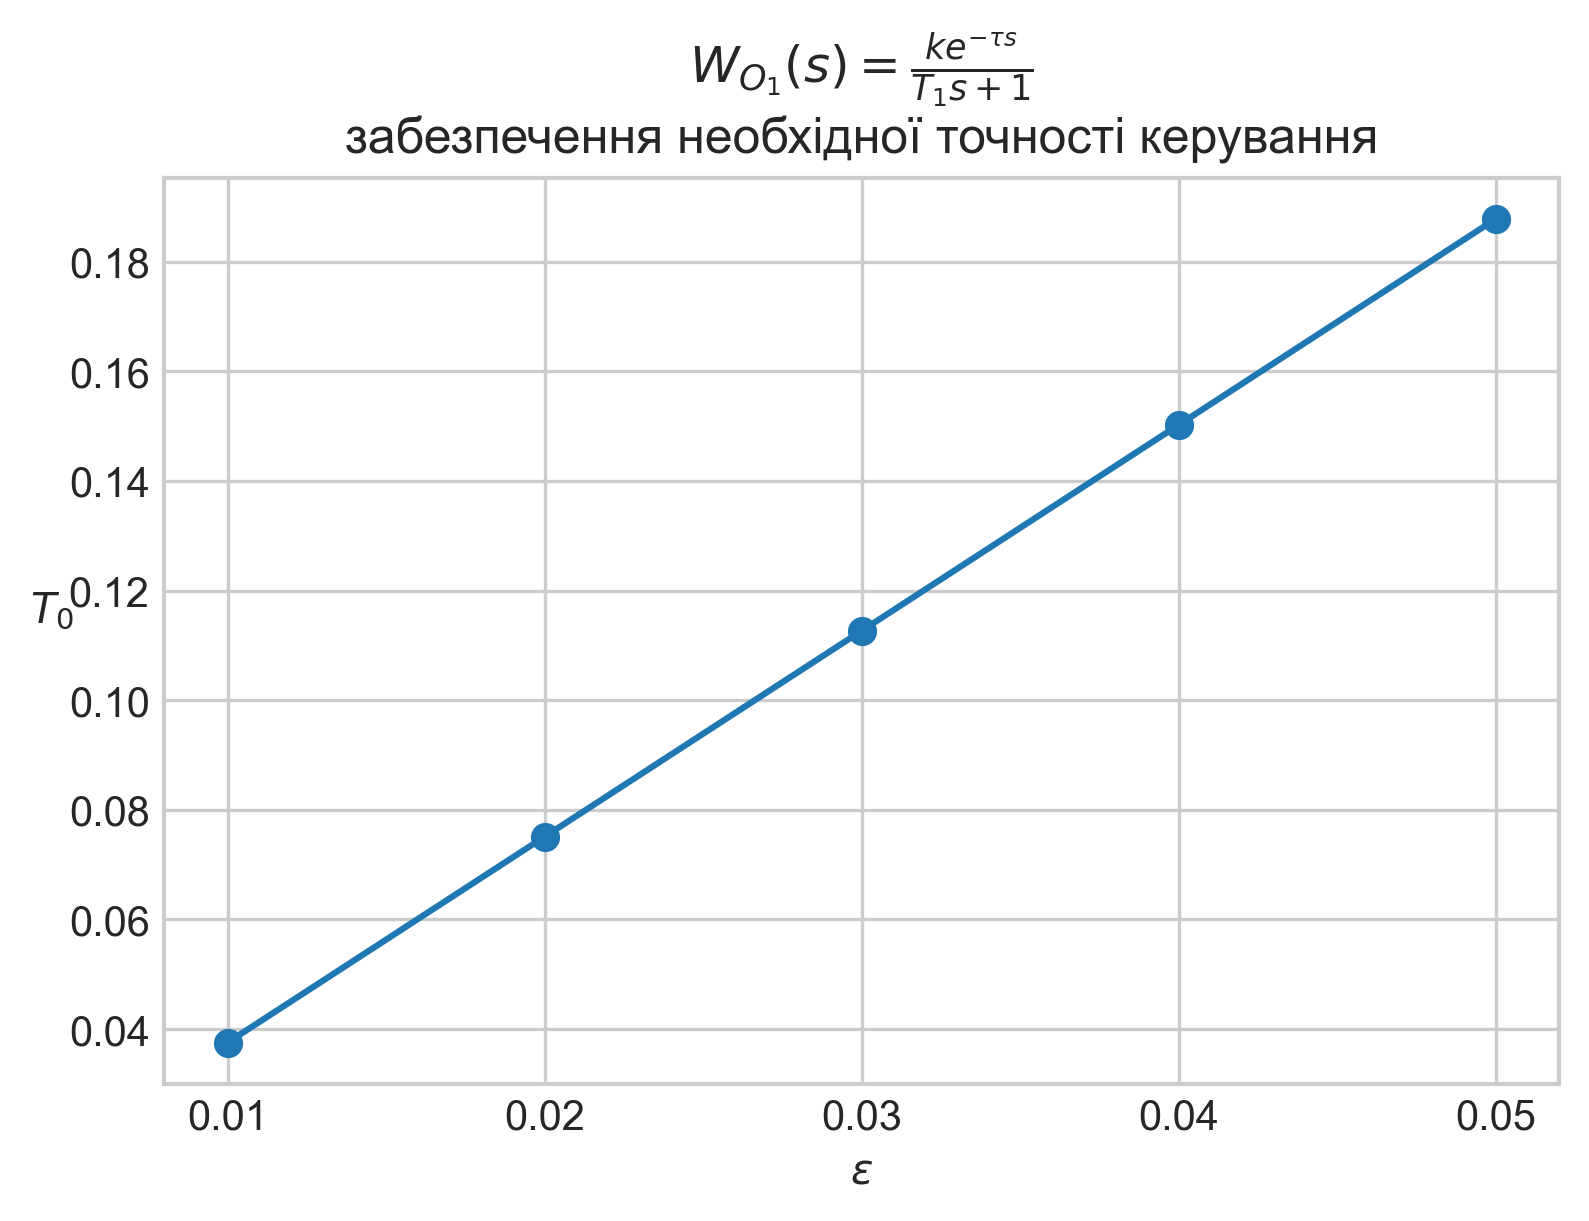
\includegraphics[scale=0.9]{pics/W_01_accur.png}
\end{center}

\subsection{Випадок \texorpdfstring{$W_{O_2}(s) = \frac{k e^{-\tau s}}{(T_1 s + 1)(T_2 s + 1)}$}{2}}
Знайдемо $B(\omega)$:
\begin{gather}
    \mbox{\normalsize $B(\omega) = \omega A(\omega) = \omega \cdot \left| W_{O_2}(j \omega)\right| = 
    \omega \cdot \frac{
        k \left| e^{-\tau j \omega}\right|
    }{
        \left|T_1 j \omega + 1\right| \left|T_2 j \omega + 1\right|
    } = \frac{k \omega}{\sqrt{\left(1 + T_1^2 \omega^2\right)\left(1 + T_2^2 \omega^2\right)}}$}
\end{gather}
$B_{\max}$ можна знайти за допомогою відповідної таблиці:
\begin{gather}
    B_{\max} = \frac{k}{T_1 + T_2} \Rightarrow T_0 = \frac{\varepsilon (T_1 + T_2)}{k}
\end{gather}
Отже, отримуємо наступні періоди квантування для різних $\varepsilon$:
\begin{center}
    \begin{tabular}{|c|c|c|c|c|c|}
        \hline
        $\varepsilon$ & $0.01$ & $0.02$ & $0.03$ & $0.04$ & $0.05$ \\
        \hline
        $T_0$ & $0.0579$ & $0.1159$ & $0.1738$ & $0.2318$ & $0.2897$ \\
        \hline
    \end{tabular}
\end{center}
Залежність $T_0$ від $\varepsilon$:
\begin{center}
    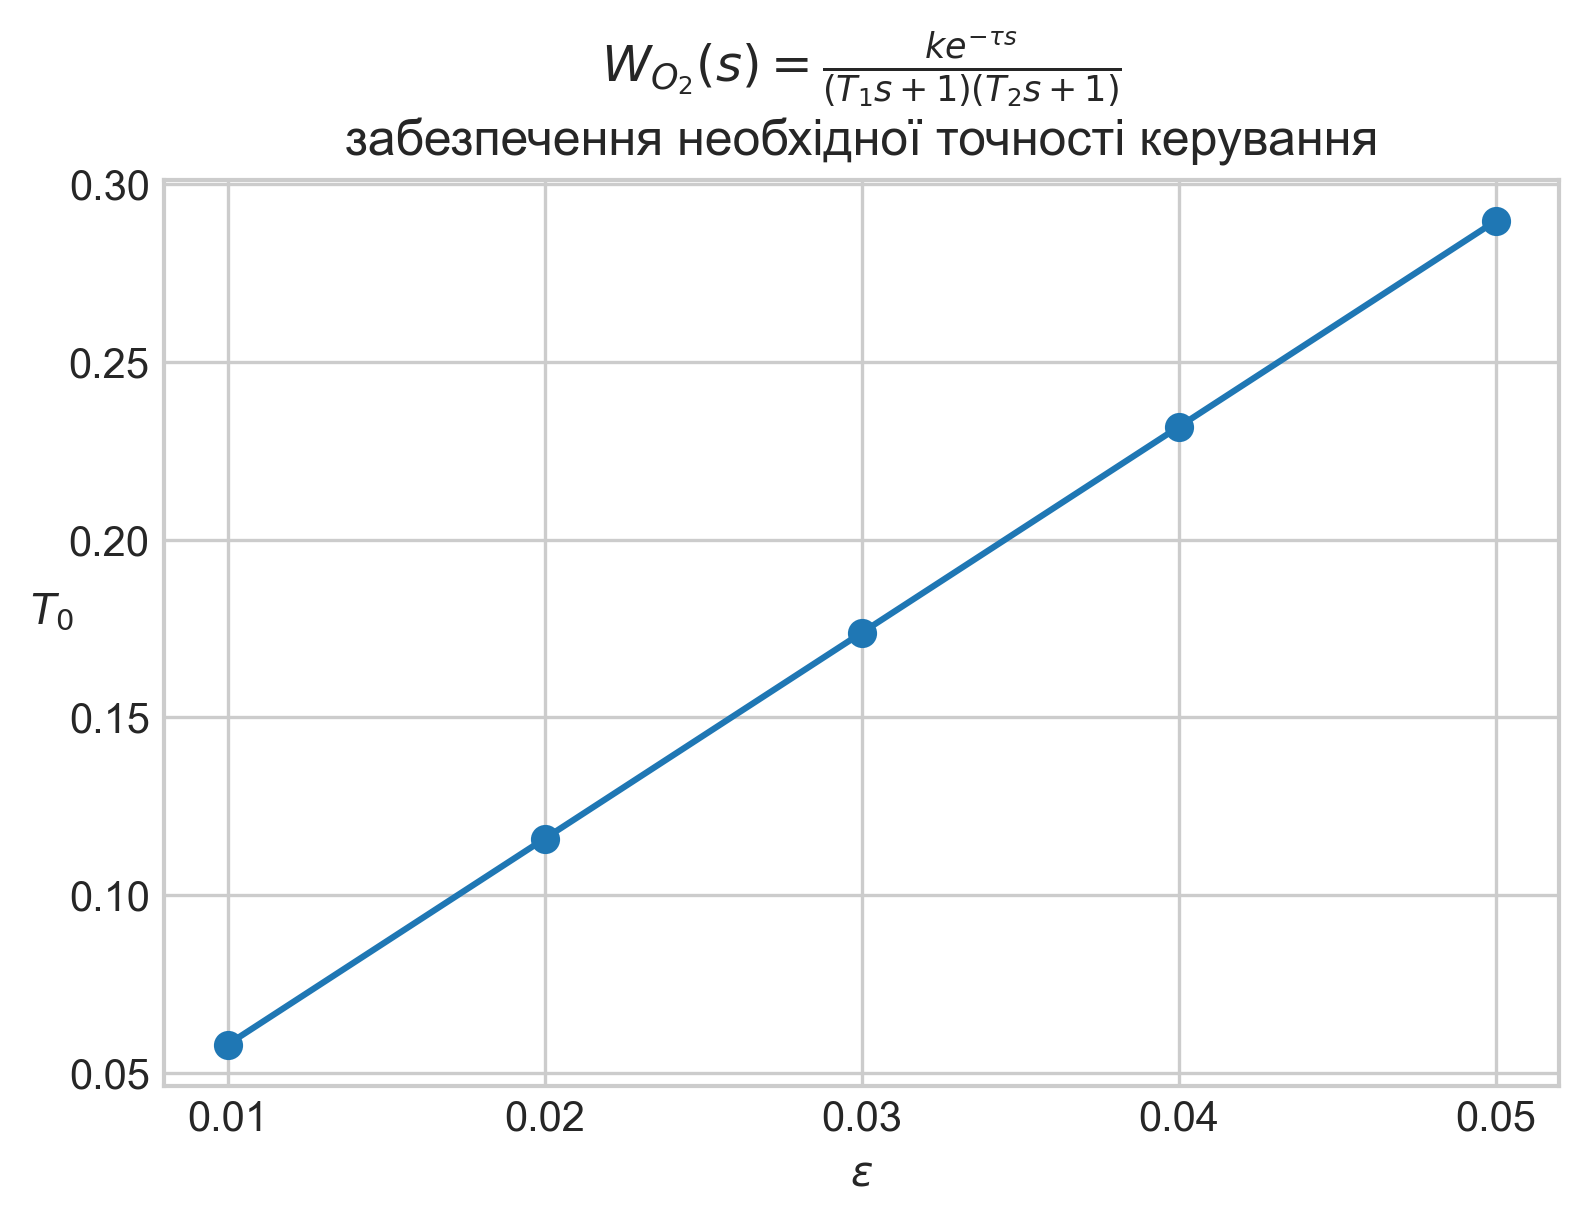
\includegraphics[scale=0.9]{pics/W_02_accur.png}
\end{center}

\section{Розрахунок за критерієм Джурі}
За цим критерієм період квантування обчислюється як $T_0 = \frac{\pi}{\omega_k}$, де 
$\omega_k$ -- розв'язок рівняння
\begin{gather}
    \left| W_{\text{з}}(j\omega_k) \right|
    = \left|
        \frac{W_O (j \omega_k) W_p (j \omega_k)}{
            1 + W_O (j \omega_k) W_p (j \omega_k)
        }
    \right| = \varepsilon
\end{gather}

\subsection{Випадок \texorpdfstring{$W_{O_1}(s) = \frac{k e^{-\tau s}}{T_1 s + 1}$}{1}}
Згідно з розділом \ref{ch:direct}, оптимальним регулятором в цьому випадку є ПІ-регулятор з передаточною функцією 
$W_p(s) = K_p \left(1 + \frac{1}{T_I s}\right) = K_p \cdot \frac{T_1 s + 1}{T_1 s}$, де $K_p = \frac{\lambda T_1}{k \left(1 + \lambda \tau\right)}$, $\lambda = \frac{1}{T_1}$, $T_I = T_1$.
Знайдемо $\left| W_{\text{з}}(j\omega) \right|$:
\begin{gather*}
    \left| W_{\text{з}}(j\omega) \right| = \frac{
        \left| W_{O_1} (j \omega) W_p (j \omega) \right|
    }{
        \left| 1 + W_{O_1} (j \omega) W_p (j \omega) \right|
    } = 
    \frac{
        \left|\frac{k e^{-\tau j \omega}}{T_1 j \omega + 1} \cdot  K_p \cdot \frac{T_1 j \omega + 1}{T_1 j \omega} \right|
    }{
        \left|1 + \frac{k e^{-\tau j \omega}}{T_1 j \omega + 1} \cdot  K_p \cdot \frac{T_1 j \omega + 1}{T_1 j \omega} \right|
    } = \\ =
    \frac{
        \left|k K_p e^{-\tau j \omega} \right|
    }{
        \left|T_1 j \omega + k K_p  e^{-\tau j \omega} \right|
    } = \frac{
        1
    }{
        \left|1 + \frac{T_1}{k K_p} j \omega e^{\tau j \omega} \right|
    } = \frac{
        1
    }{
        \left|1 + \frac{T_1}{k K_p} j \omega \left(\cos \tau\omega + j \sin \tau\omega\right) \right|
    } = \\ =
    \frac{
        1
    }{
        \left| 1 + \frac{T_1}{k K_p}
        \left(j \omega \cos \tau\omega - \omega \sin \tau\omega\right) \right|
    } = \frac{
        1
    }{
        \left| 1 - \frac{T_1}{k K_p} \omega \sin \tau\omega + 
        j \frac{T_1}{k K_p} \omega \cos \tau\omega\right|
    } = \\ = \frac{
        1
    }{
        \sqrt{
            \left(1 - \frac{T_1}{k K_p} \omega \sin \tau\omega\right)^2 +
            \left(\frac{T_1}{k K_p} \omega \cos \tau\omega\right)^2
        }
    } = \frac{
        1
    }{
        \sqrt{
            \left(\frac{T_1}{k K_p}\right)^2 \omega^2 - 2\frac{T_1}{k K_p} \omega \sin \tau\omega + 1
        }
    }
\end{gather*}
Отже, $\left| W_{\text{з}}(j\omega) \right| = \varepsilon \Leftrightarrow \left(\frac{T_1}{k K_p}\right)^2 \omega^2 - 2\frac{T_1}{k K_p} \omega \sin \tau\omega + 1 = \frac{1}{\varepsilon^2}$.
Отримуємо наступні періоди квантування для різних $\varepsilon$:
\begin{center}
    \begin{tabular}{|c|c|c|c|c|c|}
        \hline
        $\varepsilon$ & $0.01$ & $0.02$ & $0.03$ & $0.04$ & $0.05$ \\
        \hline
        $T_0$ & $1.5430$ & $3.0234$ & $4.6304$ & $5.9449$ & $7.9803$ \\
        \hline
    \end{tabular}
\end{center}
Залежність $T_0$ від $\varepsilon$:
\begin{center}
    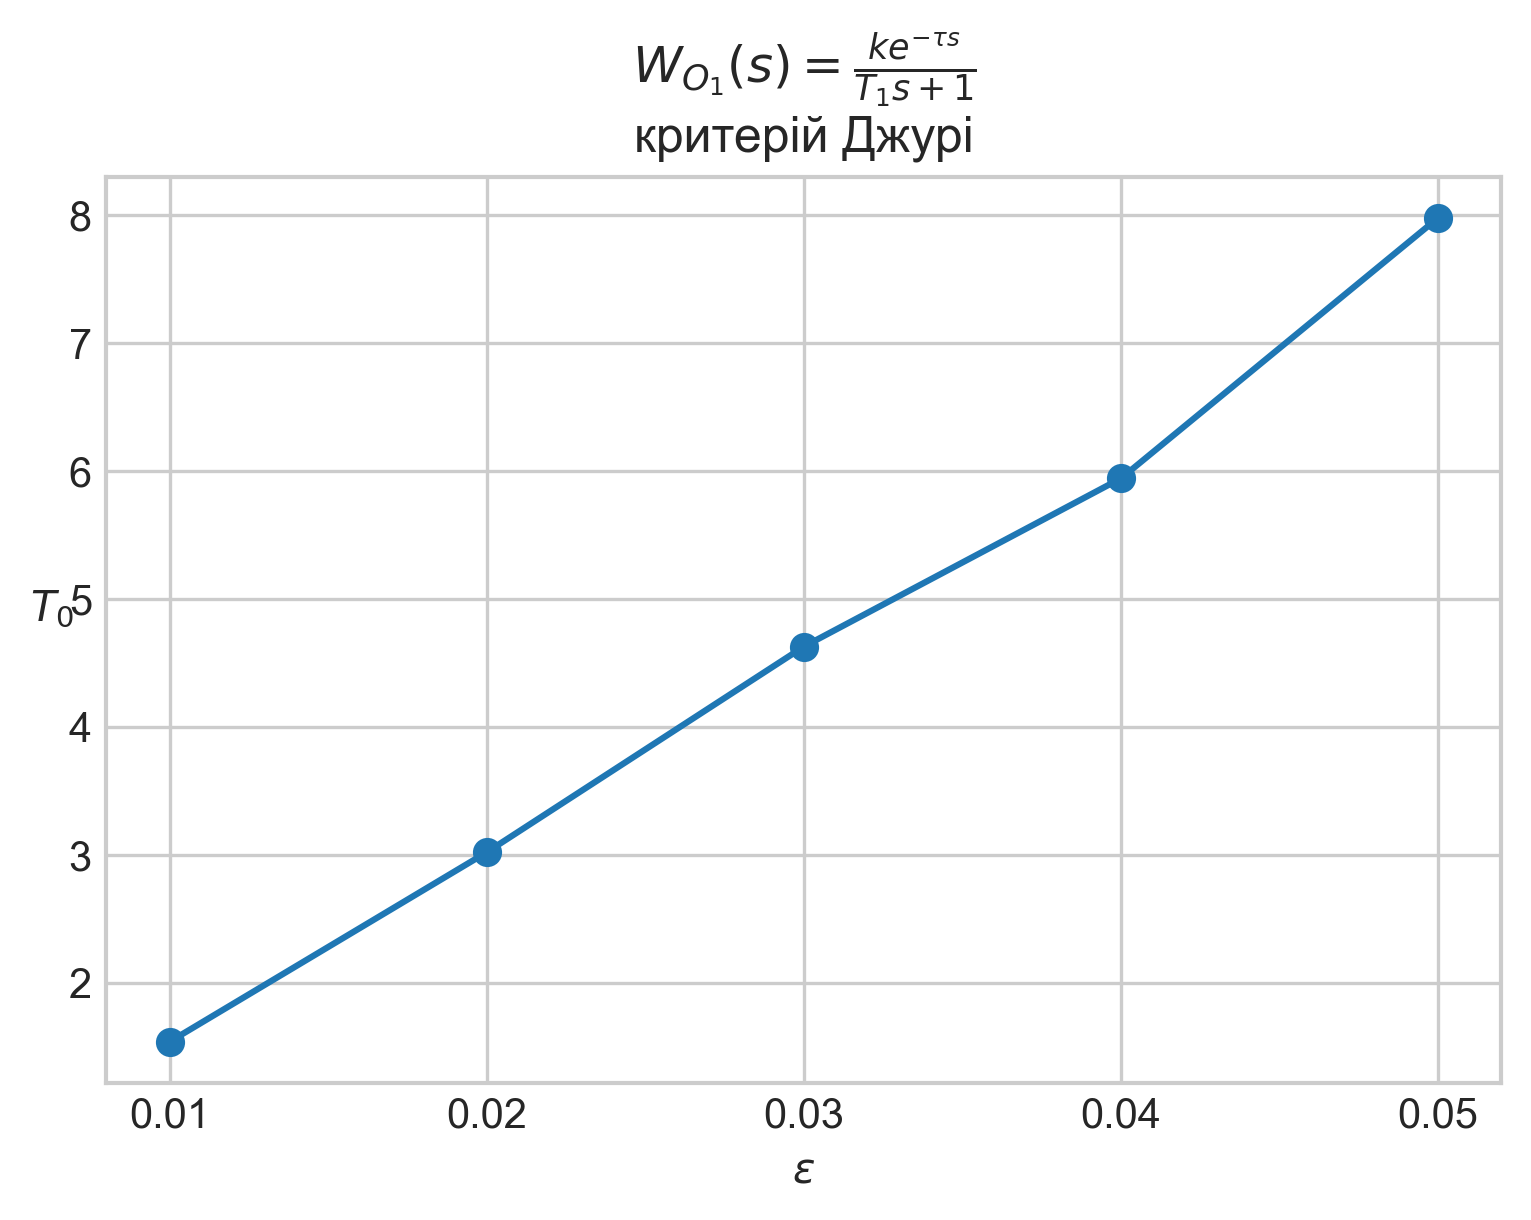
\includegraphics[scale=0.9]{pics/W_01_Jury.png}
\end{center}

\subsection{Випадок \texorpdfstring{$W_{O_2}(s) = \frac{k e^{-\tau s}}{(T_1 s + 1)(T_2 s + 1)}$}{2}}
Згідно з розділом \ref{ch:resonance}, оптимальним регулятором в цьому випадку є ПІ-регулятор з передаточною функцією 
$W_p(s) = K_p \left(1 + \frac{1}{T_I s}\right) = K_p \cdot \frac{T_1 s + 1}{T_1 s}$, де $K_p = ?$, $T_I = ?$.
Знайдемо $\left| W_{\text{з}}(j\omega) \right|$: ???

\section{Розрахунок для об'єкта з динамікою в чисельнику}
Розглядається об'єкт з передаточною функцією $W_O(s) = \frac{
    k (T_1 s + 1)
}{
    (T_2 s + 1) (T_3 s + 1)
}$. Через те, що передаточна функція має динаміку в чисельнику, критерій забезпечення необхідної точності керування
та критерій Джурі непридатні для застосування. Приведемо передаточну функцію до вигляду
$W_O(s) = \frac{K (b T s + 1)}{T^2 s^2 + 2 \nu T s + 1}$:
\begin{gather*}
    \frac{
        k (T_1 s + 1)
    }{
        (T_2 s + 1) (T_3 s + 1)
    } = \frac{k (T_1 s + 1)}{T_2 T_3 s^2 + (T_2 + T_3) s + 1}
\end{gather*}
тому $T = \sqrt{T_2 T_3} \approx 14.4568$, $b = \frac{T_1}{T} \approx 2.421$, $\nu = \frac{T_2 + T_3}{2\sqrt{T_2 T_3}} = \frac{T_2 + T_3}{2T} \approx 1.0376$.
Знайдемо $\left|W_O (j \omega)\right|$:
\begin{gather*}
    \left|W_O (j \omega)\right| = \frac{
        k \left| bT \cdot j \omega + 1 \right|
    }{
        \left| -T^2 \omega^2 + 2\nu T \cdot j \omega + 1\right|
    } = 
    \frac{
        k \sqrt{1 + b^2 T^2 \omega^2}
    }{
        \sqrt{
            \left(1 - T^2 \omega^2\right)^2 + 4 \nu^2 T^2 \omega^2
        }
    }
\end{gather*}
Введемо $\omega_{\text{зр}} = \frac{q}{T}$ -- найвищу частоту сигналу, який необхідно відновити на виході системи:
\begin{gather*}
    \left|W_O (j \omega_{\text{зр}})\right| = 
    \frac{k\sqrt{1 + b^2 q^2}}{
        \sqrt{
            \left(1 - q^2\right)^2 + 4 \nu^2 q^2
        }
    }
\end{gather*}
Розв'яжемо рівняння $\left|W_O (j \omega_{\text{зр}})\right| = \frac{1}{\theta}$, де $\theta = 31$, відносно $q$:
\begin{gather*}
    \frac{k\sqrt{1 + b^2 q^2}}{
        \sqrt{
            \left(1 - q^2\right)^2 + 4 \nu^2 q^2
        }
    } = \frac{1}{\theta} \Leftrightarrow
    \frac{1 + b^2 q^2}{1 - 2 q^2 + q^4 + 4 \nu^2 q^2} = \frac{1}{k^2 \theta^2} \Leftrightarrow \\
    \Leftrightarrow 
    1 - 2 q^2 + q^4 + 4 \nu^2 q^2 = k^2 \theta^2 \left(1 + b^2 q^2\right) \Leftrightarrow \\
    \Leftrightarrow
    q^4 + q^2 \left(4 \nu^2 - b^2 k^2 \theta^2 - 2\right) q^2 + \left(1 - k^2 \theta^2\right) = 0
\end{gather*}
Розв'яжемо це рівняння спочатку відносно $q^2$. Приблизні значення коренів: 
\begin{gather*}
    \left[
        \begin{array}{ll}
            q^2 = 489263.8397 \\
            q^2 = -0.17061
        \end{array}
    \right.
\end{gather*}
Оскільки комплексні та від'ємні $q$ не розглядаються, то отримуємо $q \approx 699.474$.
Отже, період квантування $T_0 = \frac{\pi}{\omega_{\text{зр}}} = 
\frac{\pi T}{q} = 0.0649$.
    \newpage
    % !TEX root = ../main.tex
\chapter{Визначення структури та оптимальних настройок регуляторів методом <<прямого>> синтезу}\label{ch:direct}
Розглядається об'єкт з передаточною функцією $W_{O_1}(s) = \frac{k e^{-\tau s}}{T_1 s + 1}$.
При перехідному режимі є бажаним аперіодичний перехідний процес в контурі цифрового керування,
тобто при подачі на задаюче діяння регулятора одиничного ступінчатого збурення
замкнений контур має вести себе як неперервна модель першого порядку з запізненням:
\begin{gather}
    W_{\text{з}}(s) = \frac{y(s)}{G(s)} = \frac{\lambda e^{-\tau s}}{s + \lambda}
\end{gather}

% да не хочу я это писать...

% З методичних рекомендацій маємо наступний вираз для ДПФ регулятора:
% \begin{gather}\label{reg_w01}
%     W_p(z) = \frac{
%         \left(1 - e^{-\lambda T_0}\right)
%         \left(1 - e^{-T_0 / T_1} z^{-1}\right)
%     }{
%         k
%         \left(1 - e^{-\lambda T_0} z^{-1} - \left(1 - e^{-\lambda T_0} z^{-d-1}\right) \right)
%         \left(C_1 + C_2 z^{-1}\right)
%     }
% \end{gather}
% де $a = 1 - \frac{\tau - d T_0}{T_0}$, $C_1 = 1 - e^{\frac{a T_0}{T_1}}$,
% $C_2 = e^{\frac{a T_0}{T_1}} - e^{\frac{T_0}{T_1}}$.


% Розглянемо характеристичне рівняння передаточної функції \eqref{reg_w01}:
% \begin{gather*}
%     \left(1 - e^{-\lambda T_0} z^{-1} - \left(1 - e^{-\lambda T_0} z^{-d-1}\right) \right)
%         \left(C_1 + C_2 z^{-1}\right) = 0
% \end{gather*}
% Якщо один з полюсів цього рівняння буде знаходитися в околі $z=-1$, то при аперіодичному перехідному процесі
% вихідної координати в замкненому контурі у керуючому діянні будуть коливальні процеси зі згасаючою амплітудою, які
% не є бажаними для виконавчого механізму. 
Згідно з методичними рекомендаціями, оптимальні параметри ПІ-регулятора з ДПФ 
$K_p \left(
    1 + \frac{T_0}{T_I \left(1 - z^{-1}\right)}
\right)$
визначаються за формулами
\begin{gather}\label{K_p_opt__direct}
    K_{p_{\text{опт}}} = \frac{
        1 - e^{-\lambda T_0}
    }{
        k \left(e^{T_0 / T_1} - 1\right) \left(1 + d \left(1 - e^{-\lambda T_0}\right)\right)
    } \\ \label{T_I_opt__direct}
    T_{I_{\text{опт}}} = \frac{T_0}{e^{T_0 / T_1} - 1}
\end{gather}
де $d$ -- ціла частина від ділення часу запізнення $\tau$ на період квантування
$T_0$, який беремо на основі умови забезпечення необхідної точності керування.
Візьмемо $T_0 = 0.1127$. Тоді $d = 124$, $T_{I_{\text{опт}}} = 34.9437$, а для різних варіантів $\lambda$ отримаємо такі значення $K_{p_{\text{опт}}}$:
\begin{center}
    \begin{tabular}{|c|c|}
        \hline
        $\lambda$ & $K_{p_{\text{опт}}}$ \\
        \hline
        $\frac{1}{T_1} \approx 0.0286$      & $0.0765$ \\
        \hline
        $\frac{1}{1.5T_1} \approx 0.0190$   & $0.0564$ \\
        \hline
        $\frac{1}{2T_1} \approx 0.0143$     & $0.0446$ \\
        \hline
        $\frac{1}{3T_1} \approx 0.0095$     & $0.0315$ \\
        \hline
    \end{tabular}
\end{center}
Для цифрового моделювання перехідних процесів в замкненому контурі цифрового керування зауважимо, що
можна записати рівняння
\begin{gather*}
    y(z) = W_p(z) W_{\text{п}}(z) \left(G(z) - y(z)\right) \Rightarrow
    y(z) = \frac{W_p(z) W_{\text{п}}(z)}{1 + W_p(z) W_{\text{п}}(z)} G(z) = W_{\text{з}}(z) G(z)
\end{gather*}
де $y(z)$, $G(z)$ -- $z$-перетворення від керованої координати і задаючого діяння відповідно, а 
передаточну функцію $W_{\text{з}}(z)$ було обчислено в \eqref{W_3_for_direct}.
Можна записати рекурентне рівняння, за яким буде відбуватися моделювання:
\begin{gather}
    \mbox{\small $y_n = \left(1 + e^{-T_0/T_1}\right) y_{n-1} - e^{-T_0/T_1} y_{n-2} - $} \nonumber \\
    \mbox{\small $-
    \frac{k K_{p_{\text{опт}}}}{T_I} \left(
        \left(C_1 T_{I_{\text{опт}}} + C_1 T_0\right) y_{n-d-1} + 
        \left(-C_1 T_{I_{\text{опт}}} + C_2 T_{I_{\text{опт}}} + C_2 T_0\right) y_{n-d-2} -
        C_2 T_{I_{\text{опт}}} y_{n-d-3}
    \right) +$} \nonumber \\
    \mbox{\small $+ \frac{k K_{p_{\text{опт}}}}{T_I} \left(
        \left(C_1 T_{I_{\text{опт}}} + C_1 T_0\right) g_{n-d-1} + 
        \left(-C_1 T_{I_{\text{опт}}} + C_2 T_{I_{\text{опт}}} + C_2 T_0\right) g_{n-d-2} -
        C_2 T_{I_{\text{опт}}} g_{n-d-3}
    \right)$}
\end{gather}
де $a = 1 - \frac{\tau - d T_0}{T_0}$, $C_1 = 1 - e^{-\frac{a T_0}{T_1}}$,
$C_2 = e^{-\frac{a T_0}{T_1}} - e^{-\frac{T_0}{T_1}}$, початкові умови для $y$ нульові,
а $g_n = 1$.
Отже, маємо наступні перехідні процеси для різних значень $\lambda$:
\begin{center}
    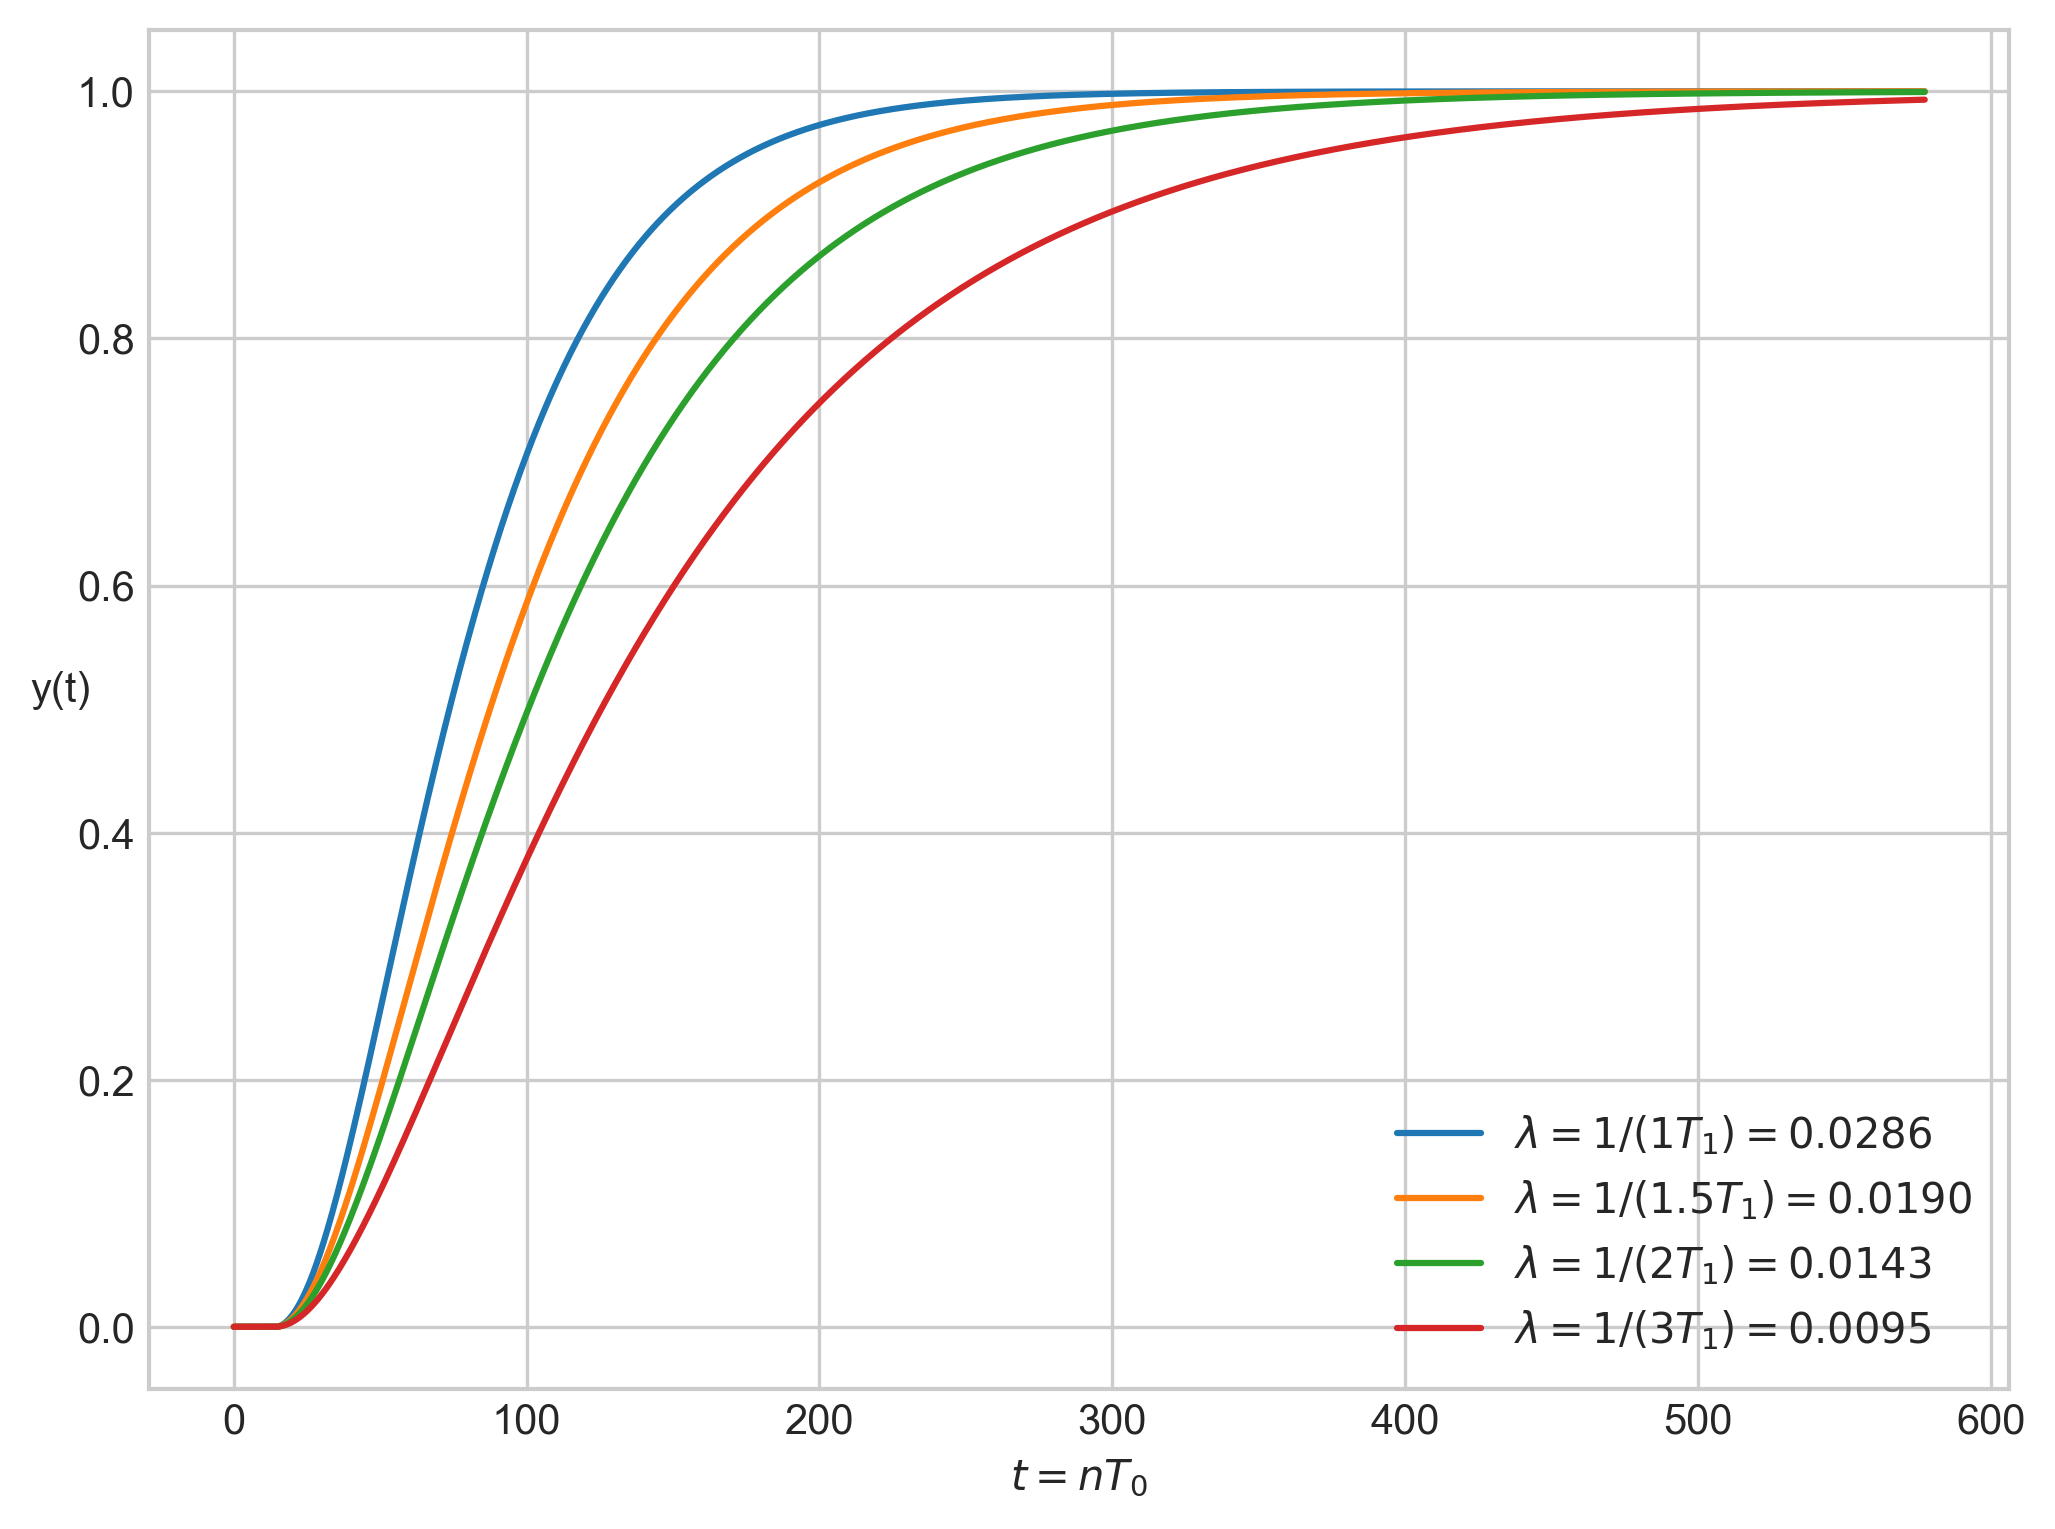
\includegraphics{pics/transient_process_task_4.png}
\end{center}
Видно, що процес зміни вихідної координати дійсно має бажаний монотонний характер.

На основі формул \eqref{K_p_opt__direct} та \eqref{T_I_opt__direct} можна визначити
оптимальні настройки для неперервного регулятора, взявши границі при $T_0 \to 0$. Отримаємо
$K_p^H = \frac{\lambda T_1}{k \left(1 + \lambda \tau\right)}$, $T_I^H = T_1$.
    \newpage
    % !TEX root = ../main.tex
\chapter{Розрахунок оптимальних параметрів ПІ-регулятора і 
періоду квантування резонансним методом}\label{ch:resonance}
За завданням, розрахунки треба провести для об'єктів з передаточними функціями
$W_O(s) = \frac{
    k e^{-\tau s}
}{
    (T_1 s + 1) (T_2 s + 1) (T_3 s + 1)
}$ \eqref{W_0} та
$
W_{O_2}(s) = \frac{k e^{-\tau s}}{(T_1 s + 1)(T_2 s + 1)}
$ \eqref{W_02}.

Регулятор цифрового керування реалізує пропорційно-інтегральний закон керування, який представлений позиційним алгоритмом:
\begin{gather*}
    u(n T_0) = K_p \left(
        e(n T_0) + \frac{T_0}{T_I} \sum_{i=1}^n e(i T_0)
    \right)
\end{gather*}
Для визначення оптимальних параметрів настройки $K_{p_{\text{опт}}}$, $T_{I_{\text{опт}}}$ та періоду квантування
$T_{0_{\text{опт}}}$ скористаємося алгоритмом, наведеним у методичних рекомендаціях до курсової роботи.

\section{Випадок \texorpdfstring{$W_O(s) = \frac{
    k e^{-\tau s}
}{
    (T_1 s + 1) (T_2 s + 1) (T_3 s + 1)
}$}{1}}
а)\;  Шляхом розв'язання відносно частоти $\omega$ нелінійного рівняння
\begin{gather}
    \arctg{\omega T_1} + \arctg{\omega T_2} + \arctg{\omega T_3} + \omega \tau = 2.62
\end{gather}
знаходимо резонансну частоту $\omega_{\varphi_H} = 0.04096$ для неперервного контура керування.

б)\;  Визначаємо верхню та нижню частоту відносно резонансної частоти неперервної системи:
$\omega_{\varphi_H}^H = \frac{\omega_{\varphi_H}}{\sqrt{2}} = 0.02897$, 
$\omega_{\varphi_H}^B = {\sqrt{2}}{\omega_{\varphi_H}} = 0.05793$.

в)\; Використовуючи знайдену частоту $\omega_{\varphi_H}$, за формулою
\begin{gather}
    A(\omega) = \frac{k}{\sqrt{\left(1+\omega^2 T_1^2\right)\left(1+\omega^2 T_2^2\right)\left(1+\omega^2 T_3^2\right)}}
\end{gather}
знаходимо другий основний динамічний параметр неперервного контура в частотній області:
$A_H\left(\omega_{\varphi_H}\right) = 3.83604$. Також, знайдемо третій основний параметр
$\Phi_H(A) = \frac{A\left(\omega_{\varphi_H}^B\right)}{A\left(\omega_{\varphi_H}^H\right)} = 0.42790$.

г)\; Використовуючи вираз 
\begin{gather}
    \varphi(\omega) = \arctg{\omega T_1} + \arctg{\omega T_2} + \arctg{\omega T_3} + \omega \tau
\end{gather}
визначаємо четвертий основний параметр в частотній області для неперервного контуру:
$\Phi_H(\varphi) = \varphi\left(\omega_{\varphi_H}^H\right) - \varphi\left(\omega_{\varphi_H}^B\right) = 1.31497$.

д)\; За емпіричними формулами визначаємо оптимальні коефіцієнти настройки неперервного ПІ-регулятора
та оптимальний період квантування:
\begin{gather}
    T_{I_{\text{опт}}}^{\text{неп}} = 
    \frac{4.061 \cdot \Phi_H(A)^{-0.3387} \cdot \Phi_H(\varphi)^{0.2075}}{\omega_{\varphi_H}} \\
    K_{p_{\text{опт}}}^{\text{неп}} = \frac{1}{2 A_H\left(\omega_{\varphi_H}\right)}
    \cdot \left(
        1 + 1.189 \cdot \Phi_H(A)^{0.7139}\cdot \left(1.852 - \Phi_H(\varphi)\right)^{0.8643}
    \right) \\
    T_{0_{\text{опт}}} = \frac{
        0.5742 \cdot \Phi_H(A)^{0.5742} \Phi_H(\varphi)^{0.9394}
    }{\omega_{\varphi_H}}
\end{gather}
Отримуємо значення
$T_{I_{\text{опт}}}^{\text{неп}} = 139.88408$, $K_{p_{\text{опт}}}^{\text{неп}} = 0.17974$,
$T_{0_{\text{опт}}} = 11.13496$.

е)\; При оптимальному періоду квантування визначаємо чотири основні параметри 
$\omega_{\varphi}$, $A\left(\omega_{\varphi}\right)$, $\Phi(A)$, $\Phi(\varphi)$
в частотній області при врахуванні ПНЧ об'єкта. Для цього використаємо рівняння
\begin{gather}\label{A_w_1}
    A(\omega) = A_H(\omega) \cdot \frac{
        \sin {\frac{\omega T_{0_{\text{опт}}}}{2}}
    }{
        {\frac{\omega T_{0_{\text{опт}}}}{2}}
    } \\ \label{phi_w_1}
    \varphi(\omega) = 
    \arctg{\omega T_1} + \arctg{\omega T_2} + \arctg{\omega T_3} + \omega \tau + {\frac{\omega T_{0_{\text{опт}}}}{2}}
\end{gather}
Шляхом розв'язання $\varphi(\omega) = 2.62$ знаходимо частоту 
$\omega_{\varphi} = 0.03670$, а потім за рівняннями \eqref{A_w_1}, \eqref{phi_w_1} знаходимо 
$A\left(\omega_{\varphi}\right) = 4.32464$, 
$\Phi(A) = \frac{A\left(\omega_{\varphi_H}^B\right)}{A\left(\omega_{\varphi_H}^H\right)} = 0.46223$, 
$\Phi(\varphi) = \varphi\left(\omega_{\varphi_H}^H\right) - \varphi\left(\omega_{\varphi_H}^B\right) = 1.39902$.

ж)\; При оптимальному періоді квантування $T_{0_{\text{опт}}}$ знаходимо 
оптимальні значення $T_{I_{\text{опт}}}$ та $K_{p_{\text{опт}}}$ за формулами
\begin{gather}
    T_{I_{\text{опт}}} = 
    \frac{4.061 \cdot \Phi(A)^{-0.3387} \cdot \Phi(\varphi)^{0.2075}}{\omega_{\varphi}} \\
    K_{p_{\text{опт}}} = \frac{1}{2 A\left(\omega_{\varphi_H}\right)}
    \cdot \left(
        1 + 1.189 \cdot \Phi(A)^{0.7139}\cdot \left(1.852 - \Phi(\varphi)\right)^{0.8843}
    \right)
\end{gather}
Отримуємо значення
$T_{I_{\text{опт}}} = 154.07932$, $K_{p_{\text{опт}}} = 0.15558$.

Зберемо результати обчислень до таблиці:
\begin{center}
    \begin{tabular}{|c|c|}
        \hline
        параметр & значення \\
        \hline
        $\omega_{\varphi_H}$ & 0.04096\\
        \hline
        $\omega_{\varphi_H}^H$ & 0.02897\\
        \hline
        $\omega_{\varphi_H}^BH$ & 0.05793\\
        \hline
        $A_H\left(\omega_{\varphi_H}\right)$ & 3.83604\\
        \hline
        $\Phi_H(A)$ & 0.42790\\
        \hline
        $\Phi_H(\varphi)$ & 1.31497\\
        \hline
        $T_{I_{\text{опт}}}^{\text{неп}}$ & 139.88408\\
        \hline
        $K_{p_{\text{опт}}}^{\text{неп}}$ & 0.17974\\
        \hline
        $T_{0_{\text{опт}}}$ & 11.13496\\
        \hline
        $\omega_{\varphi}$ & 0.03670\\
        \hline
        $A\left(\omega_{\varphi}\right)$ & 4.32464\\
        \hline
        $\Phi(A)$ & 0.46223\\
        \hline
        $\Phi(\varphi)$ & 1.39902\\
        \hline
        $T_{I_{\text{опт}}}$ & 154.07932\\
        \hline
        $K_{p_{\text{опт}}}$ & 0.15558\\
        \hline
     \end{tabular}
\end{center}
Для цифрового моделювання перехідного процесу вихідної координати $y$ скористаємося передаточною функцією $W_\text{з}(s)$:
\begin{gather*}
    \mbox{\normalsize $y(s) = W_\text{з}(s) G(s) = \frac{W_p(s) W_O(s)}{1 + W_p(s) W_O(s)} G(s)$} \\
    \mbox{\normalsize $W_p(s) = K_{p_{\text{опт}}} \left(1 + \frac{1}{T_{I_{\text{опт}}} s}\right), \;
    G(s) = \frac{1}{s} \left(1 - e^{-s T_{0_{\text{опт}}}}\right)$}
\end{gather*}

Чисельно знайшовши обернене перетворення Лапласа від $y(s)$ в моменти $n T_{0_{\text{опт}}}$, 
отримаємо значення вихідної координати при подачі на задаюче діяння одиничного імпульсу довжиною $T_{0_{\text{опт}}}$. 
Відношення затухання дорівнює $\frac{B}{A} = 0.16958$.
\begin{center}
    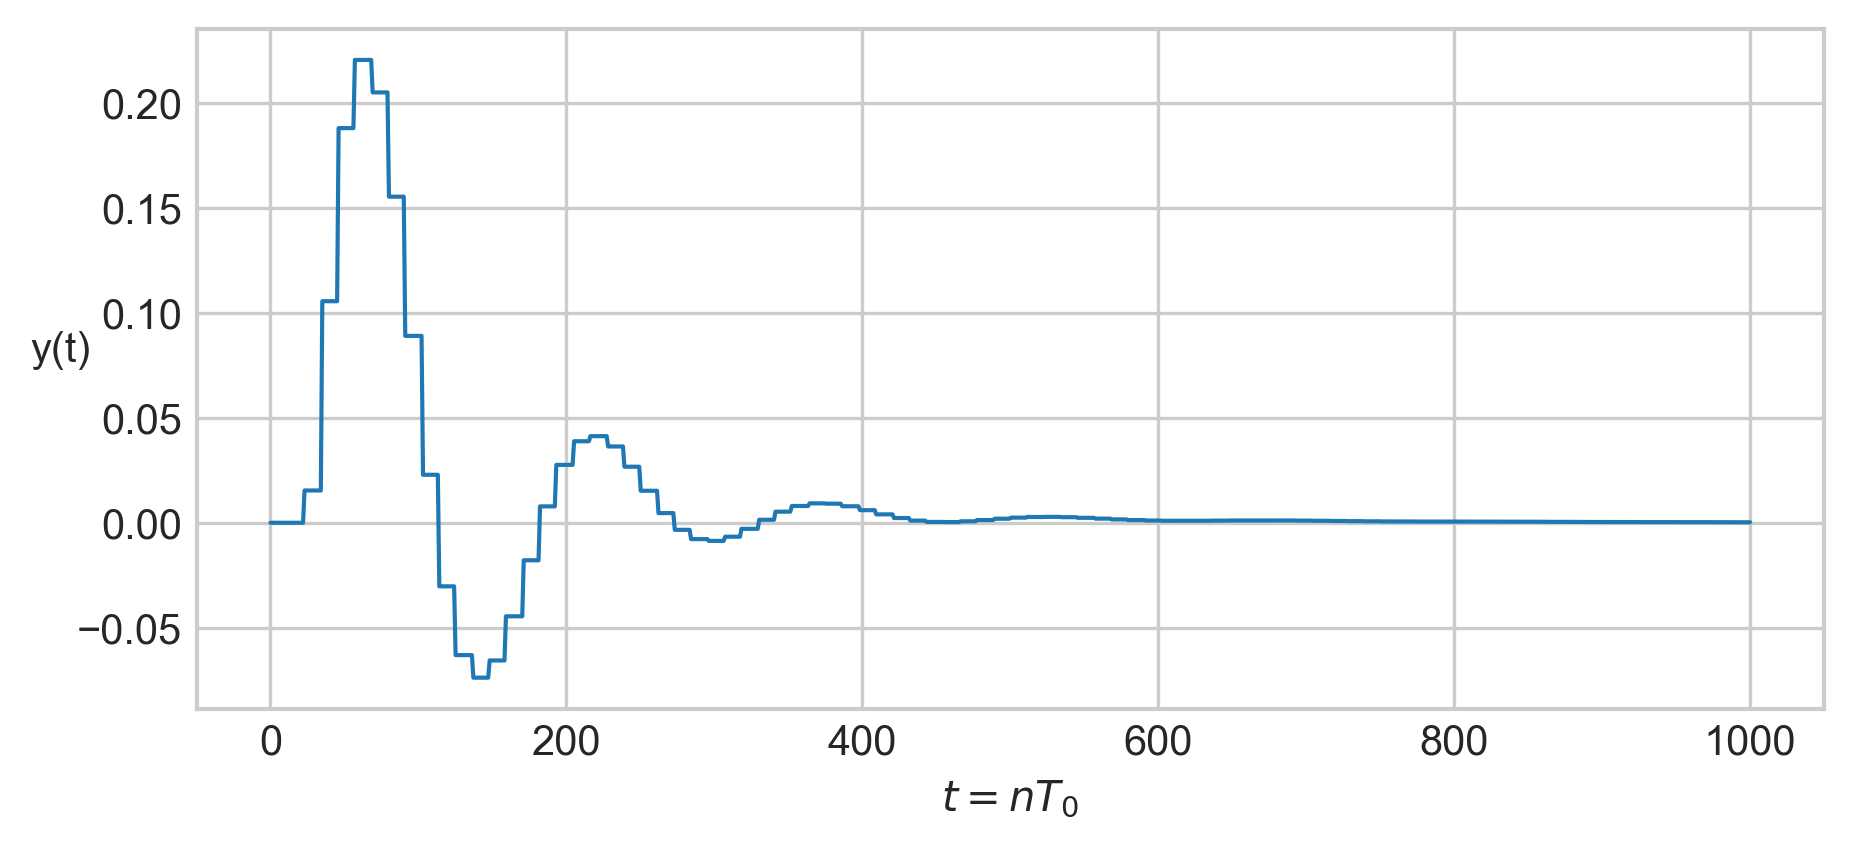
\includegraphics[scale=0.75]{pics/transient_process_task_5_1.png}
\end{center}

\section{Випадок \texorpdfstring{$W_{O_2}(s) = \frac{k e^{-\tau s}}{(T_1 s + 1)(T_2 s + 1)}$}{2}}
а)\;  Шляхом розв'язання відносно частоти $\omega$ нелінійного рівняння
\begin{gather}
    \arctg{\omega T_1} + \arctg{\omega T_2} + \omega \tau = 2.62
\end{gather}
знаходимо резонансну частоту $\omega_{\varphi_H} = 0.05341$ для неперервного контура керування.

б)\;  Визначаємо верхню та нижню частоту відносно резонансної частоти неперервної системи:
$\omega_{\varphi_H}^H = \frac{\omega_{\varphi_H}}{\sqrt{2}} = 0.03777$, 
$\omega_{\varphi_H}^B = {\sqrt{2}}{\omega_{\varphi_H}} = 0.07553$.

в)\; Використовуючи знайдену частоту $\omega_{\varphi_H}$, за формулою
\begin{gather}
    A(\omega) = \frac{k}{\sqrt{\left(1+\omega^2 T_1^2\right)\left(1+\omega^2 T_2^2\right)\left(1+\omega^2 T_3^2\right)}}
\end{gather}
знаходимо другий основний динамічний параметр неперервного контура в частотній області:
$A_H\left(\omega_{\varphi_H}\right) = 3.08583$. Також, знайдемо третій основний параметр
$\Phi_H(A) = \frac{A\left(\omega_{\varphi_H}^B\right)}{A\left(\omega_{\varphi_H}^H\right)} = 0.41264$.

г)\; Використовуючи вираз 
\begin{gather}
    \varphi(\omega) = \arctg{\omega T_1} + \arctg{\omega T_2} + \arctg{\omega T_3} + \omega \tau
\end{gather}
визначаємо четвертий основний параметр в частотній області для неперервного контуру:
$\Phi_H(\varphi) = \varphi\left(\omega_{\varphi_H}^H\right) - \varphi\left(\omega_{\varphi_H}^B\right) = 1.15456$.

д)\; За емпіричними формулами визначаємо оптимальні коефіцієнти настройки неперервного ПІ-регулятора
та оптимальний період квантування:
\begin{gather}
    T_{I_{\text{опт}}}^{\text{неп}} = 
    \frac{4.061 \cdot \Phi_H(A)^{-0.3387} \cdot \Phi_H(\varphi)^{0.2075}}{\omega_{\varphi_H}} \\
    K_{p_{\text{опт}}}^{\text{неп}} = \frac{1}{2 A_H\left(\omega_{\varphi_H}\right)}
    \cdot \left(
        1 + 1.189 \cdot \Phi_H(A)^{0.7139}\cdot \left(1.852 - \Phi_H(\varphi)\right)^{0.8643}
    \right) \\
    T_{0_{\text{опт}}} = \frac{
        0.5742 \cdot \Phi_H(A)^{0.5742} \Phi_H(\varphi)^{0.9394}
    }{\omega_{\varphi_H}}
\end{gather}
Отримуємо значення
$T_{I_{\text{опт}}}^{\text{неп}} = 105.72649$, $K_{p_{\text{опт}}}^{\text{неп}} = 0.23703$,
$T_{0_{\text{опт}}} = 7.40205$.

е)\; При оптимальному періоду квантування визначаємо чотири основні параметри 
$\omega_{\varphi}$, $A\left(\omega_{\varphi}\right)$, $\Phi(A)$, $\Phi(\varphi)$
в частотній області при врахуванні ПНЧ об'єкта. Для цього використаємо рівняння
\begin{gather}\label{A_w_2}
    A(\omega) = A_H(\omega) \cdot \frac{
        \sin {\frac{\omega T_{0_{\text{опт}}}}{2}}
    }{
        {\frac{\omega T_{0_{\text{опт}}}}{2}}
    } \\ \label{phi_w_2}
    \varphi(\omega) = 
    \arctg{\omega T_1} + \arctg{\omega T_2} + \arctg{\omega T_3} + \omega \tau + {\frac{\omega T_{0_{\text{опт}}}}{2}}
\end{gather}
Шляхом розв'язання $\varphi(\omega) = 2.62$ знаходимо частоту 
$\omega_{\varphi} = 0.04792$, а потім за рівняннями \eqref{A_w_1}, \eqref{phi_w_1} знаходимо 
$A\left(\omega_{\varphi}\right) = 3.51065$, 
$\Phi(A) = \frac{A\left(\omega_{\varphi_H}^B\right)}{A\left(\omega_{\varphi_H}^H\right)} = 0.43618$, 
$\Phi(\varphi) = \varphi\left(\omega_{\varphi_H}^H\right) - \varphi\left(\omega_{\varphi_H}^B\right) = 1.23981$.

ж)\; При оптимальному періоді квантування $T_{0_{\text{опт}}}$ знаходимо 
оптимальні значення $T_{I_{\text{опт}}}$ та $K_{p_{\text{опт}}}$ за формулами
\begin{gather}
    T_{I_{\text{опт}}} = 
    \frac{4.061 \cdot \Phi(A)^{-0.3387} \cdot \Phi(\varphi)^{0.2075}}{\omega_{\varphi}} \\
    K_{p_{\text{опт}}} = \frac{1}{2 A\left(\omega_{\varphi_H}\right)}
    \cdot \left(
        1 + 1.189 \cdot \Phi(A)^{0.7139}\cdot \left(1.852 - \Phi(\varphi)\right)^{0.8843}
    \right)
\end{gather}
Отримуємо значення
$T_{I_{\text{опт}}} = 117.36092$, $K_{p_{\text{опт}}} = 0.20311$.

Зберемо результати обчислень до таблиці:
\begin{center}
    \begin{tabular}{|c|c|}
        \hline
        параметр & значення \\
        \hline
        $\omega_{\varphi_H}$ & 0.05341\\
        \hline
        $\omega_{\varphi_H}^H$ & 0.03777\\
        \hline
        $\omega_{\varphi_H}^BH$ & 0.07553\\
        \hline
        $A_H\left(\omega_{\varphi_H}\right)$ & 3.08583\\
        \hline
        $\Phi_H(A)$ & 0.41264\\
        \hline
        $\Phi_H(\varphi)$ & 1.15456\\
        \hline
        $T_{I_{\text{опт}}}^{\text{неп}}$ & 105.72649\\
        \hline
        $K_{p_{\text{опт}}}^{\text{неп}}$ & 0.23703\\
        \hline
        $T_{0_{\text{опт}}}$ & 7.40205\\
        \hline
        $\omega_{\varphi}$ & 0.04792\\
        \hline
        $A\left(\omega_{\varphi}\right)$ & 3.51065\\
        \hline
        $\Phi(A)$ & 0.43618\\
        \hline
        $\Phi(\varphi)$ & 1.23981\\
        \hline
        $T_{I_{\text{опт}}}$ & 117.36092\\
        \hline
        $K_{p_{\text{опт}}}$ & 0.20311\\
        \hline
     \end{tabular}
\end{center}
Цифрове моделювання перехідного процесу вихідної координати $y$ проведемо аналогічно попередньому пункту. Коефіцієнт затухання дорівнює 
$\frac{B}{A} = 0.35151$.
\begin{center}
    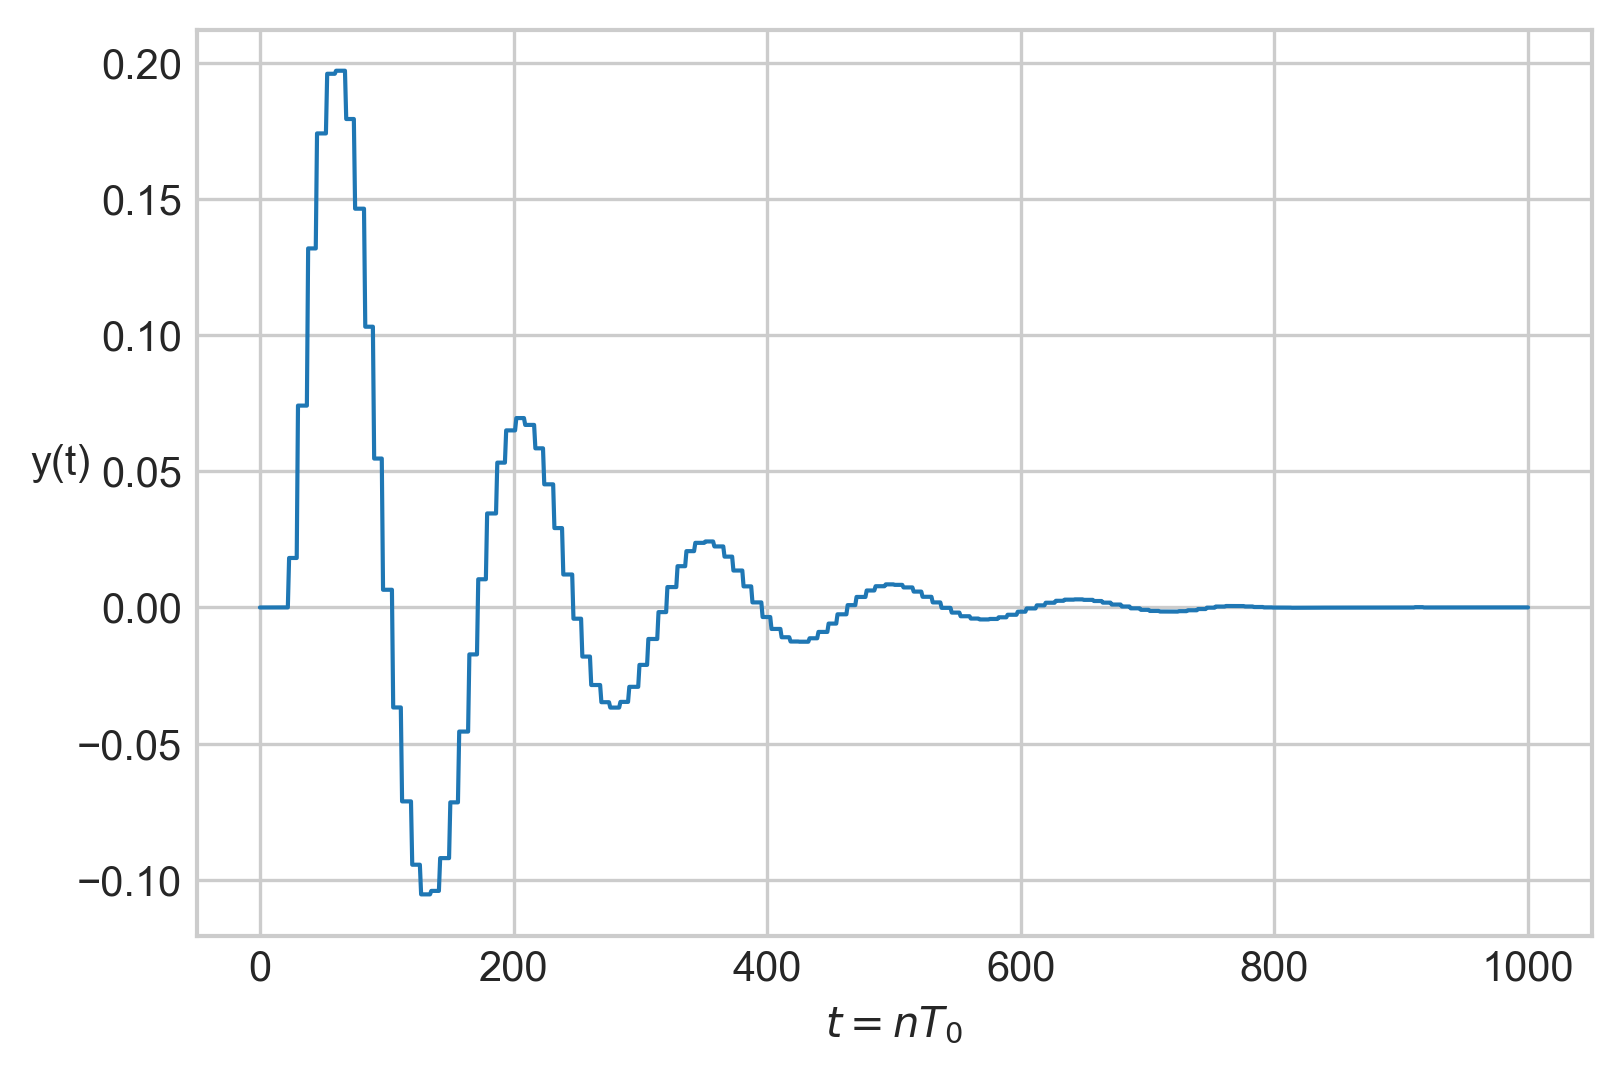
\includegraphics[scale=0.75]{pics/transient_process_task_5_2.png}
\end{center}
    \newpage
    % !TEX root = ../main.tex
\chapter{Синтез лінійно-квадратичного регулятора стану}
Розглянемо математичну модель об'єкта у вигляді передаточної функції
\begin{gather*}
    W_O(s) = \frac{y(s)}{u(s)} = \frac{
    k
    }{
        (T_1 s + 1) (T_2 s + 1) (T_3 s + 1)
    } = \\ = \frac{
        k
    }{
        T_1 T_2 T_3 s^3 + \left(T_1 T_2 + T_1 T_3 + T_2 T_3\right) s^2
        + \left(T_1 + T_2 + T_3\right) s + 1
    }
\end{gather*}
Введемо нові коефіцієнти 
\begin{gather*}
    a_1 = \frac{T_1 T_2 + T_1 T_3 + T_2 T_3}{T_1 T_2 T_3} = 0.17211, 
    a_2 = \frac{T_1 + T_2 + T_3}{T_1 T_2 T_3} = 0.00889 \\
    a_3 = \frac{1}{T_1 T_2 T_3} = 0.00014, 
    b = \frac{k}{T_1 T_2 T_3} = 0.00127
\end{gather*}
після чого цю передаточну функцію можна записати наступним чином:
\begin{gather*}
    W_O(s) = \frac{b}{s^3 + a_1 s^2 + a_2 s + a_3} = \frac{y(s)}{u(s)}
\end{gather*}
Введемо нову змінну $X(s) = \frac{u(s)}{s^3 + a_1 s^2 + a_2 s + a_3} = \frac{y(s)}{b}$, звідки
\begin{gather*}
    u(s) = \left(s^3 + a_1 s^2 + a_2 s + a_3\right) X(s)
\end{gather*}
Виконавши зворотнє перетворення Лапласа, отримаємо
\begin{gather*}
    \frac{d^3 x(t)}{dt^3} = u(t) - a_1 \frac{d^2 x(t)}{dt^2} - a_2 \frac{d x(t)}{dt} - a_3 x(t)
\end{gather*}
Введемо фазові змінні $x_1(t) = x(t)$, $x_2(t) = \frac{d x(t)}{dt}$, $x_3(t) = \frac{d^2 x(t)}{dt^2}$,
причому $\frac{d x_1(t)}{dt} = x_2(t)$, $\frac{d x_2(t)}{dt} = x_3(t)$,
$\frac{d x_3(t)}{dt} = -a_3 x_1(t) - a_2 x_2(t) - a_1 x_3(t) + u(t)$. Запишемо ці рівності у векторно-матричній формі:
\begin{gather}\label{eq:state_space}
    \begin{bmatrix}
        \frac{d x_1(t)}{dt} \\ \frac{d x_2(t)}{dt} \\ \frac{d x_3(t)}{dt}
    \end{bmatrix} = 
    \begin{bmatrix}
        0 & 1 & 0 \\
        0 & 0 & 1 \\
        -a_3 & -a_2 & -a_1
    \end{bmatrix}
    \begin{bmatrix}
        x_1 \\ x_2 \\ x_3
    \end{bmatrix} + 
    \begin{bmatrix}
        0 \\ 0 \\ 1
    \end{bmatrix} u(t)
    \Leftrightarrow
    \frac{d \vec{x}(t)}{dt} = A \vec{x}(t) + \vec{b} u(t)
\end{gather}
Виконаємо дискретизацію рівняння \eqref{eq:state_space}, використавши період квантування,
який було визначено в резонансному методі ($T_0 = 11.13496$):
\begin{gather}
    \vec{x}\left(\left[k+1\right]T_0\right) = F \vec{x}\left(kT_0\right) + \vec{g} u\left(k T_0\right)
\end{gather}
де $F = e^{A T_0}$, $\vec{g} = \int_0^{T_0} e^{A t} \vec{b} dt = A^{-1} \left(e^{A T_0} - I\right) \vec{b}$.
Обчислимо значення $F$ та $\vec{g}$:
\begin{gather*}
    F = \begin{pmatrix}
        0.98025  & 9.79083  & 33.05948 \\
        -0.00452 & 0.68649  & 4.1009 \\
        -0.00056 & -0.04096 & -0.01933
    \end{pmatrix}, \;
    \vec{g} = \begin{pmatrix}
        144.46778 \\ 33.05948 \\ 4.1009
    \end{pmatrix}
\end{gather*}

Синтез лінійно-квадратичного регулятора стану 
\begin{gather}\label{eq:lin_quad_reg}
    u\left(k T_0\right) = -\vec{K}_p \vec{x}\left(k T_0\right) = 
    - \begin{bmatrix}
        K_1 & K_2 & K_3
    \end{bmatrix}
    \begin{bmatrix}
        x_1\left(k T_0\right) \\
        x_2\left(k T_0\right) \\
        x_3\left(k T_0\right)
    \end{bmatrix}
\end{gather}
виконаємо за рекурентною процедурою
\begin{gather*}
    \vec{K}_p (k) = \left(q_3 + \vec{g}^T L\left([k+1]T_0\right) \vec{g}\right)^{-1}
    \vec{g}^T L\left((k+1)T_0\right) F \\
    L\left(k T_0\right) = F^T L\left([k+1]T_0\right) F + Q_2 - 
    F^T L\left([k+1]T_0\right) \vec{g} \cdot \vec{K}_p (k)
\end{gather*}
при початковому значенні матриці $L\left(n T_0\right) = Q_1$, де вагові матриці
$Q_1$, $Q_2$ та коефіцієнт $q_3$ обираються для забезпечення швидкості мінімізації квадратичного критерію оптимальності
\begin{gather*}
    I = \vec{x}^T \left(nT_0\right) Q_1 \vec{x} \left(nT_0\right) + 
    \sum_{k=0}^{n-1} \left(
        \vec{x}^T \left(k T_0\right) Q_2 \vec{x} \left(k T_0\right) + q_3 u^2 \left(k T_0\right)
    \right)
\end{gather*}

За наведеною рекурентною процедурою отримаємо 
\begin{gather*}
    \vec{K}_p = \begin{bmatrix}
        0.00278 & 0.03643 & 0.15089
    \end{bmatrix}
\end{gather*}
На основі рівнянь \eqref{eq:state_space} та \eqref{eq:lin_quad_reg}
маємо рівняння стану замкненої системи:
\begin{gather*}
    \vec{x}\left([k+1]T_0\right) = \left(F - \vec{g} \cdot \vec{K}_p \right) \vec{x}\left(kT_0\right)
\end{gather*}
Користуючись цим рівнянням, змоделюємо поведінку системи при різних ненульових початкових умовах:
\begin{center}
    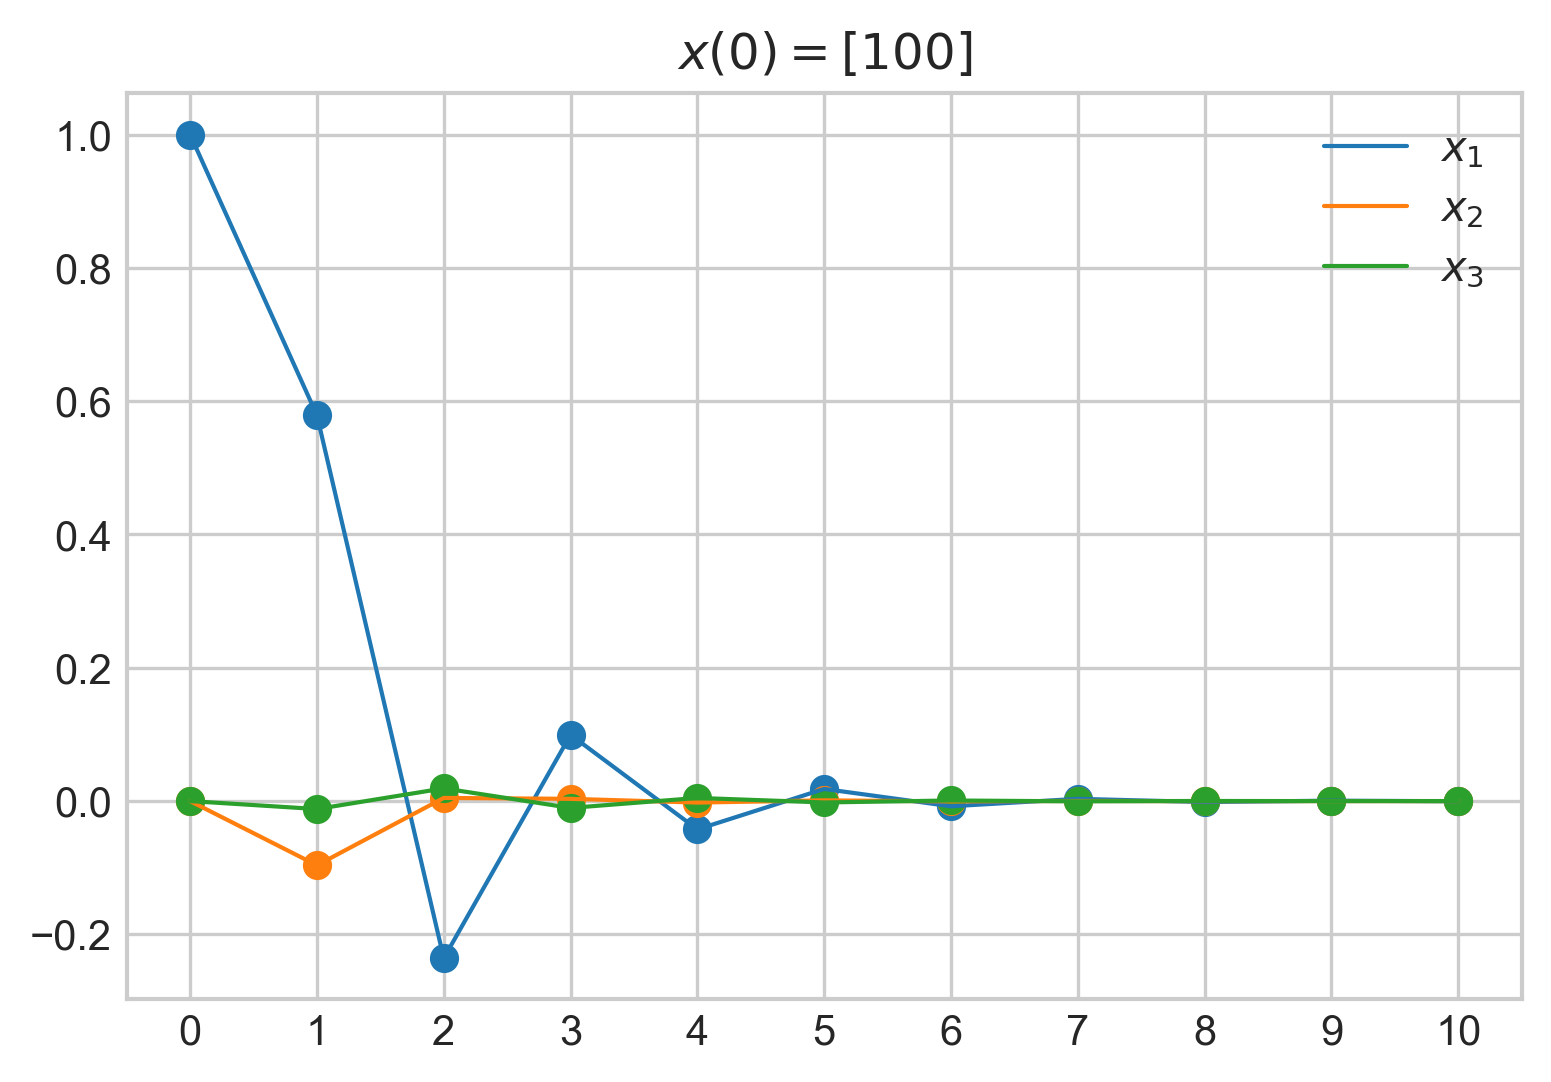
\includegraphics[scale=0.9]{pics/lin_quad_model_[1 0 0].png} \\
    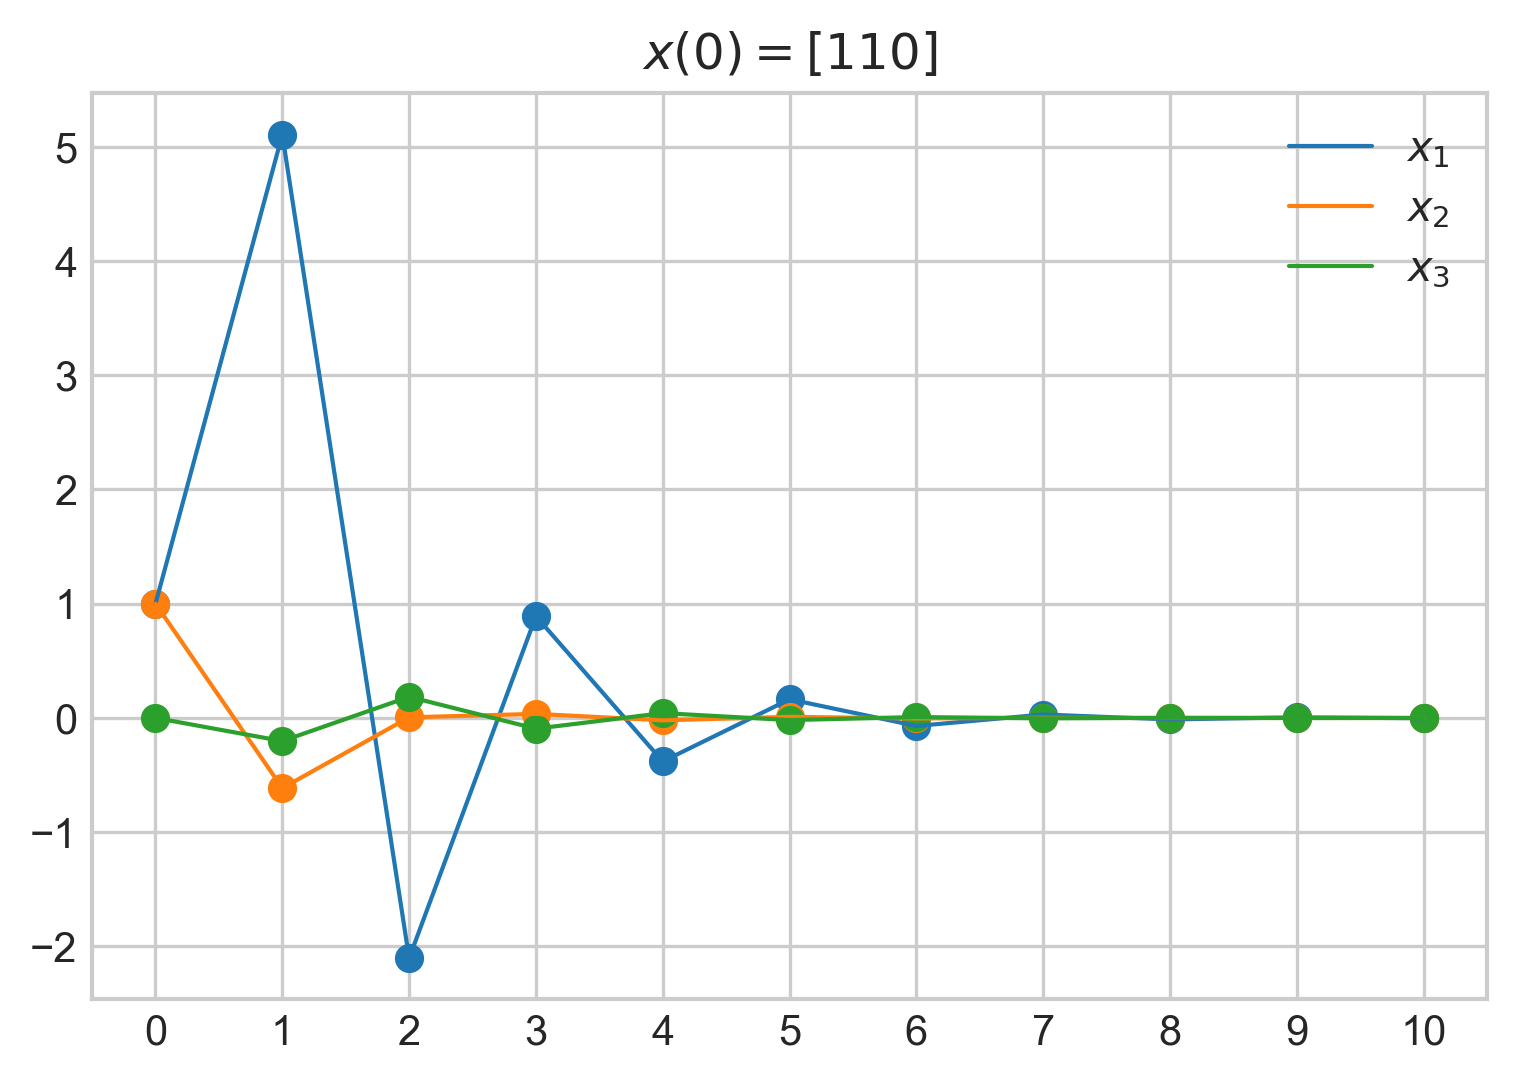
\includegraphics[scale=0.9]{pics/lin_quad_model_[1 1 0].png} \\
    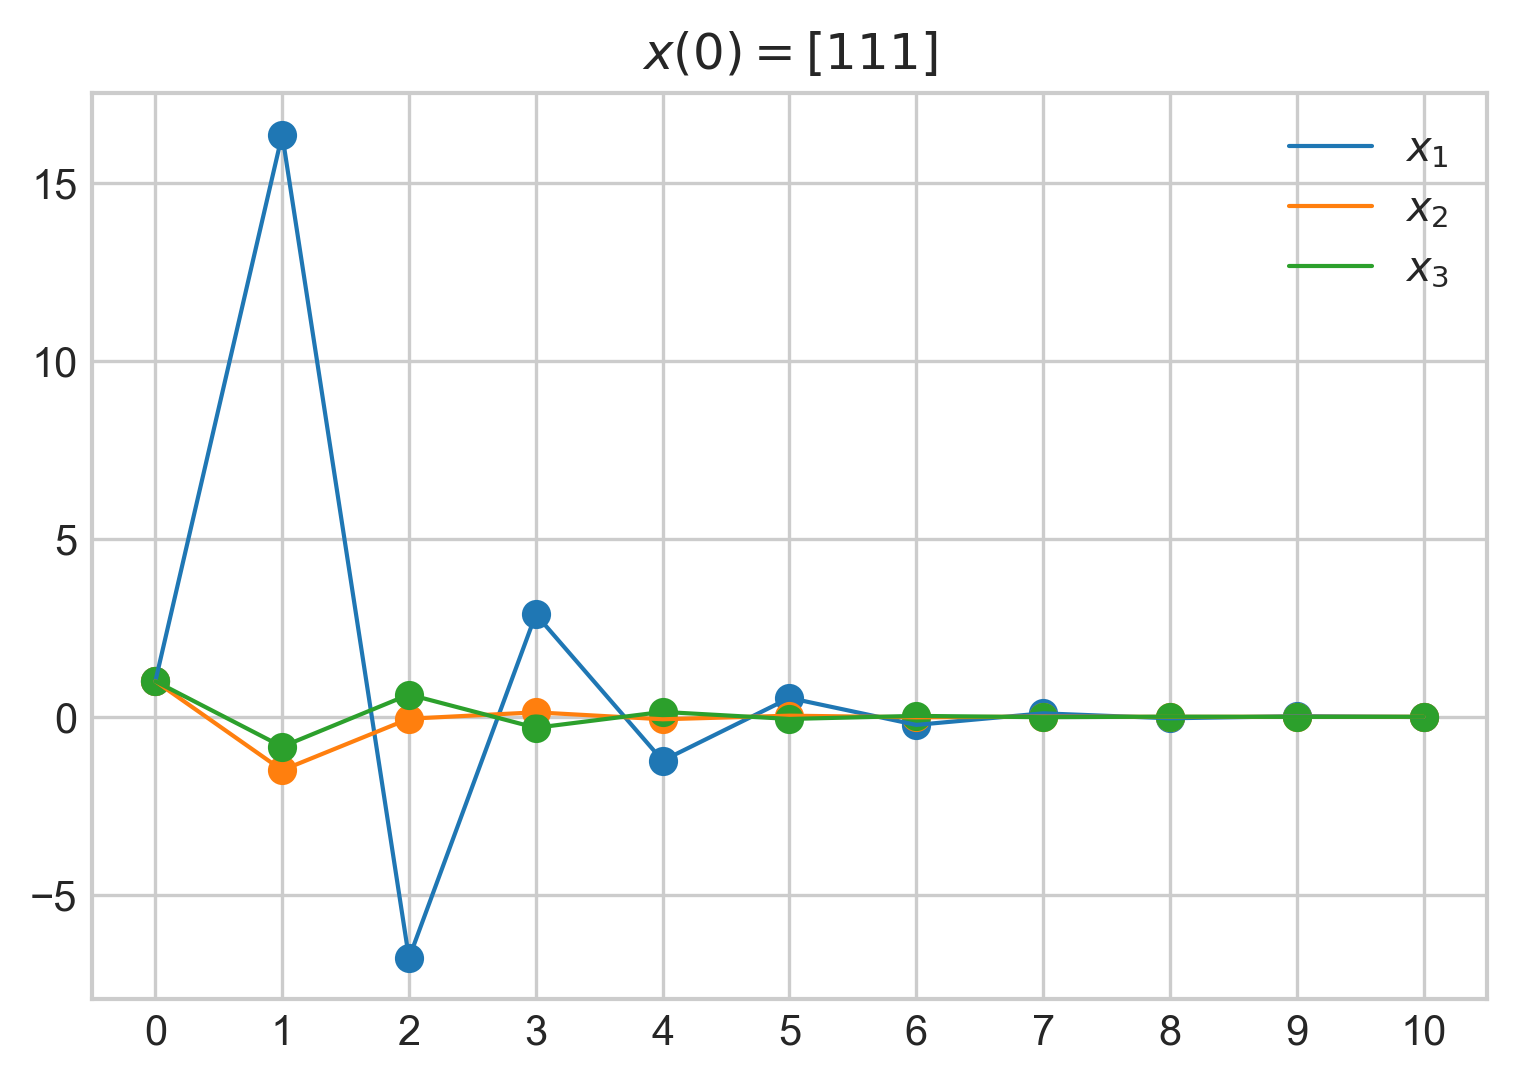
\includegraphics[scale=0.9]{pics/lin_quad_model_[1 1 1].png}
\end{center}
    \newpage
    % !TEX root = ../main.tex
\chapter{Дослідження стійкості}
Дослідимо стійкість контура цифрового керування
з передаточною функцією об'єкта $W_O(s) = \frac{k e^{-\tau s}}{T_1 s + 1}$
та ПІ-регулятором, що має дискретну передаточну функцію
$W_p(z) = K_p \left(1 + \frac{T_0}{T_I \left(1 - z^{-1}\right)}\right)$.
Взявши період квантування $T_0 = 1.5430$, отриманий методом Джурі
у пункті \ref{jury_for_stability}, за 
формулами \eqref{K_p_opt__direct} та \eqref{T_I_opt__direct}
при $\lambda = \frac{1}{T_1}$
визначимо оптимальні настройки ПІ-регулятора :
\begin{gather*}
    K_{p_{\text{опт}}} = 34.2342, T_{I_{\text{опт}}} = 0.0740
\end{gather*}

\section{Критерій Гурвіца}
Розрахунок стійкості замкненої системи цифрового керування 
проведемо за послідовністю, наведеною у методичних рекомендаціях.

а)\; $d$ -- ціле число від ділення часу запізнення на період квантування $T_0$, воно дорівнює 9.

б)\; За формулою \eqref{transfer_function_for_stability} обчислимо дискретну передаточну функцію приведеної неперервної частини:
\begin{gather*}
    W_\text{п}(z) = \frac{
        0.37311 z^{-10} + 0.02884 z^{-11}
    }{
        1 - e^{-0.04409} z^{-1}
    }
\end{gather*}

в)\; Визначимо характеристичне рівняння замкненого контуру:
\begin{gather}
    1 + W_p(z)W_\text{п}(z) = 0 \Leftrightarrow \nonumber \\ \Leftrightarrow
    z^{12} -1.95687 z^{11} + 0.95687 z^10 + 0.02881 z^2 -0.02537 z -0.00213 = 0 \label{hurwitz_char_pol}
\end{gather}

г)\; Застосуємо $w$-перетворення до \eqref{hurwitz_char_pol}, підставивши $z = \frac{1+w}{1-w}$:
\begin{gather}
    3.96579 w^{12} + 38.76510 w^{11} + 178.70561 w^{10} + 470.05698 w^9 + 835.79917 w^8 + \nonumber \\ 
    + 1004.10086 w^7 + 839.23167 w^6 + 494.18403 w^5 + 181.65973 w^4 + 45.12629 w^3 + \nonumber \\
    + 4.26842 w^2 + 0.13504 w + 0.00131 = 0 \label{hurwitz_char_pol_in_w}
\end{gather}

д)\; Складемо для полінома з \eqref{hurwitz_char_pol_in_w} матрицю Гурвіца та перевіримо додатність усіх діагональних мінорів. Матриця Гурвіца має вигляд

\begin{gather*}
    \mbox{\tiny
    $
    \left[\begin{array}{cccccccccccc}
        38.7651 & 470.057 & 1004.1009 & 494.184 & 45.1263 & 0.135 & 0.0 & 0.0 & 0.0 & 0.0 & 0.0 & 0.0 \\
        3.9658 & 178.7056 & 835.7992 & 839.2317 & 181.6597 & 4.2684 & 0.0013 & 0.0 & 0.0 & 0.0 & 0.0 & 0.0 
        \\0.0 & 38.7651 & 470.057 & 1004.1009 & 494.184 & 45.1263 & 0.135 & 0.0 & 0.0 & 0.0 & 0.0 & 0.0 
        \\0.0 & 3.9658 & 178.7056 & 835.7992 & 839.2317 & 181.6597 & 4.2684 & 0.0013 & 0.0 & 0.0 & 0.0 & 0.0 
        \\0.0 & 0.0 & 38.7651 & 470.057 & 1004.1009 & 494.184 & 45.1263 & 0.135 & 0.0 & 0.0 & 0.0 & 0.0 
        \\0.0 & 0.0 & 3.9658 & 178.7056 & 835.7992 & 839.2317 & 181.6597 & 4.2684 & 0.0013 & 0.0 & 0.0 & 0.0 
        \\0.0 & 0.0 & 0.0 & 38.7651 & 470.057 & 1004.1009 & 494.184 & 45.1263 & 0.135 & 0.0 & 0.0 & 0.0 
        \\0.0 & 0.0 & 0.0 & 3.9658 & 178.7056 & 835.7992 & 839.2317 & 181.6597 & 4.2684 & 0.0013 & 0.0 & 0.0 
        \\0.0 & 0.0 & 0.0 & 0.0 & 38.7651 & 470.057 & 1004.1009 & 494.184 & 45.1263 & 0.135 & 0.0 & 0.0 
        \\0.0 & 0.0 & 0.0 & 0.0 & 3.9658 & 178.7056 & 835.7992 & 839.2317 & 181.6597 & 4.2684 & 0.0013 & 0.0 
        \\0.0 & 0.0 & 0.0 & 0.0 & 0.0 & 38.7651 & 470.057 & 1004.1009 & 494.184 & 45.1263 & 0.135 & 0.0 
        \\0.0 & 0.0 & 0.0 & 0.0 & 0.0 & 3.9658 & 178.7056 & 835.7992 & 839.2317 & 181.6597 & 4.2684 & 0.0013
    \end{array}\right]
    $
    }
\end{gather*}
Комп'ютерне обчислення показує, що усі діагональні мінори є додатними. Це означає, що усі корені рівняння \eqref{hurwitz_char_pol_in_w}
мають від'ємні дійсні частини, а отже, усі корені рівняння \eqref{hurwitz_char_pol} за модулем менше одиниці, що свідчить про стійкість
контуру, що розглядається.

\section{Аналог критерію Михайлова}
Для застосування аналогу критерію Михайлова розглянемо поліном з рівняння \eqref{hurwitz_char_pol} (який одразу записано з коефіцієнтом 1 перед старшим степенем).
Підставимо $z = e^{j \omega T_0} = \cos \left(\omega T_0\right) + j \sin \left(\omega T_0\right)$:
\begin{gather*}
    F(z) = z^n + a_{n-1} z^{n-1} + \dots + a_1 z + a_0 \Rightarrow \\
    \Rightarrow F\left(e^{j \omega T_0}\right) = 
    e^{j \omega n T_0} + a_{n-1} e^{j \omega (n-1) T_0} + \dots + a_1 e^{j \omega T_0} + a_0 = \\ =
    \left[
        \cos \left(\omega n T_0\right) + a_{n-1} \cos \left(\omega (n-1) T_0\right) + \dots + a_1 \cos \left(\omega T_0\right) + a_0
    \right] + \\ +
    j \left[
        \sin \left(\omega n T_0\right) + a_{n-1} \sin \left(\omega (n-1) T_0\right) + \dots + a_1 \sin \left(\omega T_0\right)
    \right] = u (\omega) + j v (\omega)
\end{gather*}
Побудуємо годограф $F\left(e^{j \omega T_0}\right)$ при зміні частоти в межах $0 \leq \omega \leq \frac{\pi}{T_0}$:
\begin{center}
    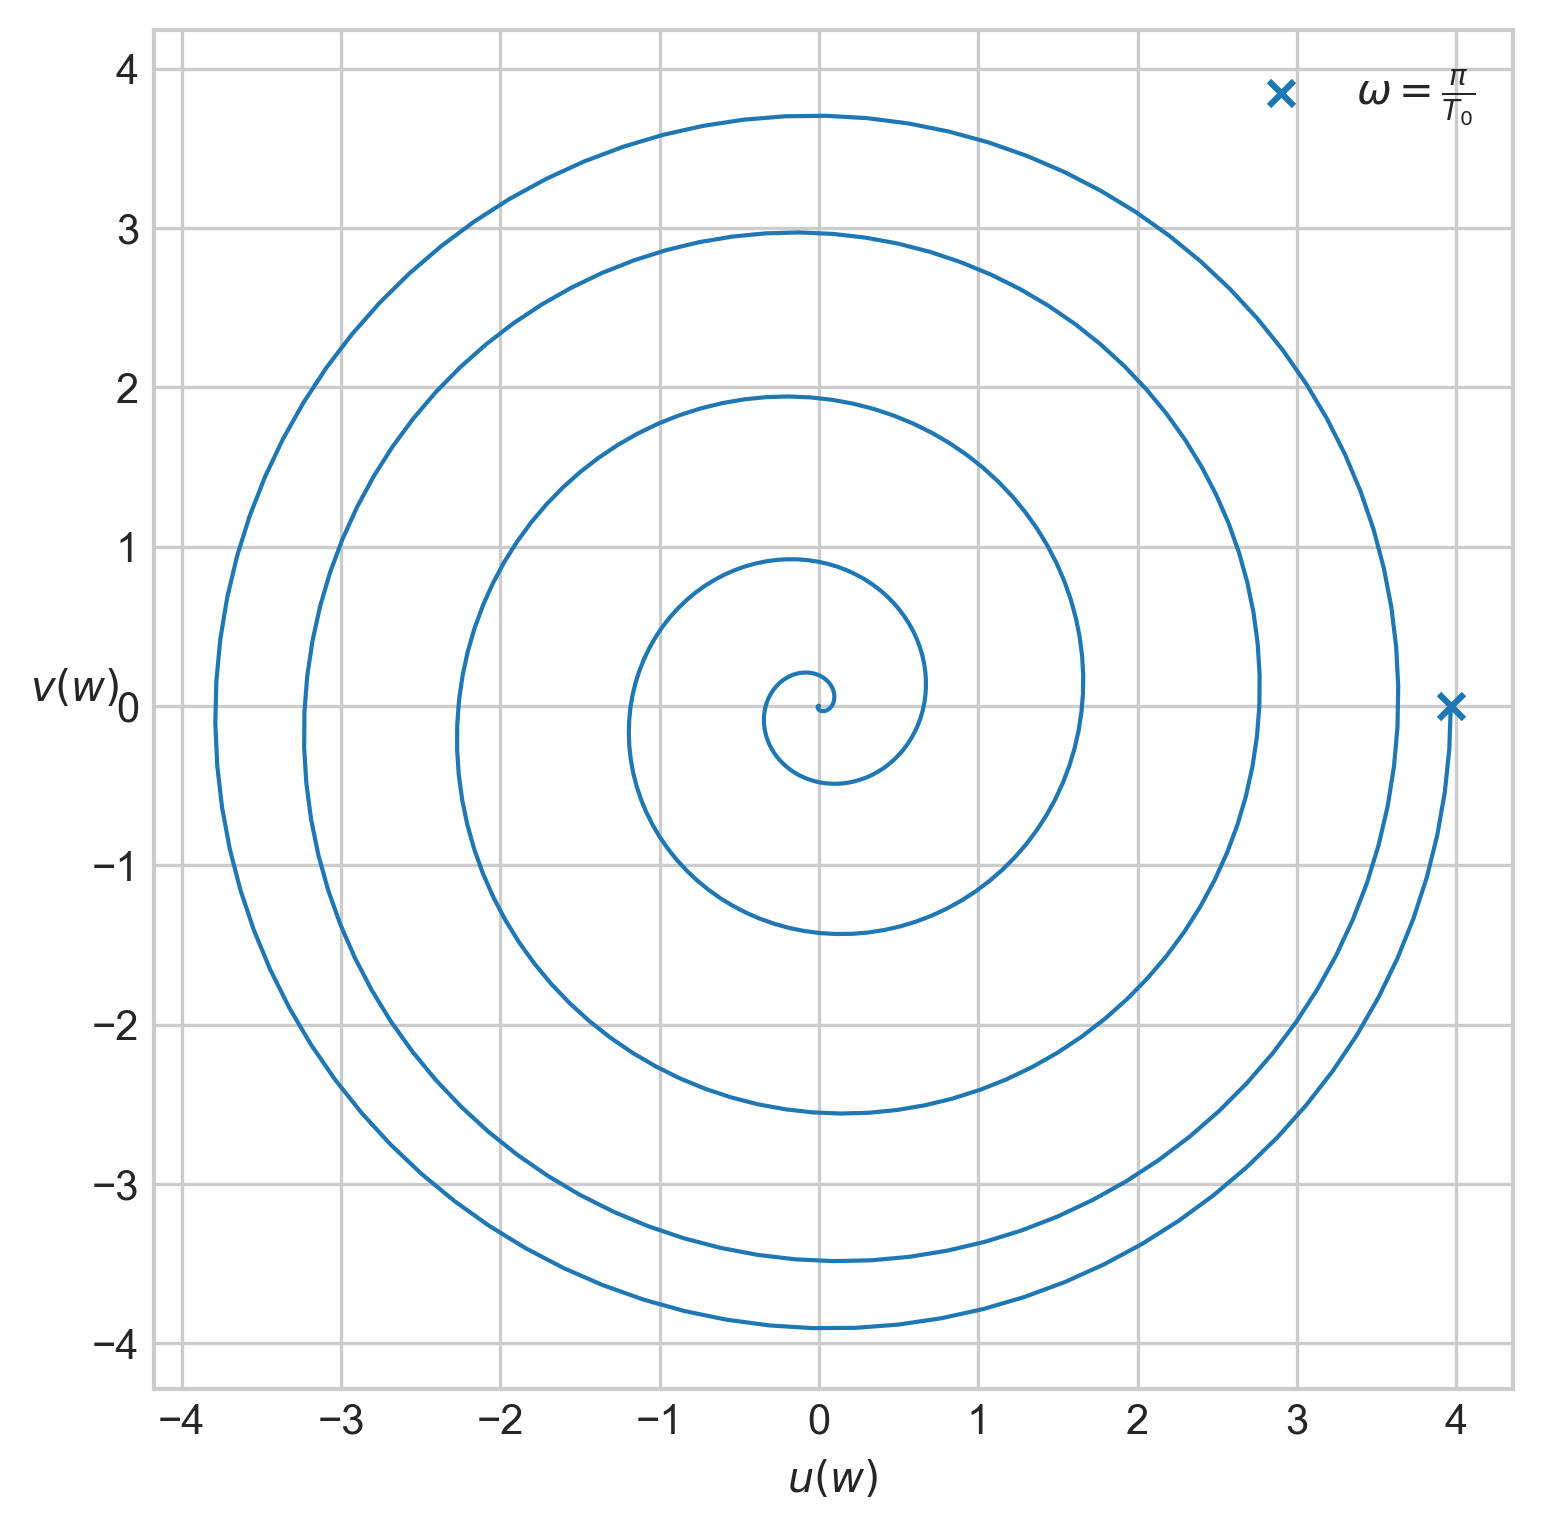
\includegraphics{pics/hodograph.png}
\end{center}
Можна порахувати, що годограф пройшов $2\cdot 12 = 24$ квадранти, тому контур є стійким.
    \newpage
    % !TEX root = ../main.tex
\chapter{Алгоритми цифрового керування}
\section{Позиційний алгоритм}
У даному алгоритмі регулятор цифрового керування виконує розрахунок повної величини
керуючого діяння у формі \eqref{PID}. Віднявши з обох частин $u\left([n-1] T_0\right)$,
отримаємо рівняння
\begin{gather*}
    \mbox{\normalsize $u\left[n T_0\right] - u\left[(n-1) T_0\right] = K_p \left(
        e\left[n T_0\right] - e\left[(n-1) T_0\right]
    \right) + 
    \frac{K_p T_0}{T_I} e\left[n T_0\right] + $}
    \\ 
    \mbox{\normalsize $ + \frac{K_p T_D}{T_0} \left(
        e\left[n T_0\right] - 2e\left[(n-1) T_0\right] + e\left[(n-2) T_0\right]
    \right)$}
\end{gather*}
яке можна записати як
\begin{gather}\label{PID:pos_alg}
    u\left[n T_0\right] = u\left[(n-1) T_0\right] + 
    A_0 \cdot e\left[n T_0\right] + A_1 \cdot e\left[(n-1) T_0\right] + A_2 \cdot e\left[(n-2) T_0\right]
\end{gather}
де $A_0 = K_p \left(1 + \frac{T_0}{T_I} + \frac{T_D}{T_0}\right)$,
$A_1 = -K_p \left(1 + 2\frac{T_D}{T_0}\right)$, $A_3 = \frac{K_p T_D}{T_0}$, а похибка визначається як
$e\left[n T_0\right] = G\left[n T_0\right] - y\left[n T_0\right]$.
Отримане рівняння \eqref{PID:pos_alg} є зручною для програмування на комп'ютері формою рівняння
\eqref{PID}.
Обчислимо значення коефіцієнтів $A_0, A_1, A_2$ для систем з розрахованими настройками ПІ-регулятора.
Оскільки $T_D = 0$, то вирази спрощуються до $A_ 0 = K_p\left(1 + \frac{T_0}{T_I}\right)$,
$A_1 = -K_p$, $A_2 = 0$.
\begin{center}
    \begin{tabular}{|c|c|c|}
        \hline
        об'єкт, метод & $A_0$ & $A_1$ \\
        \hline
        $W_O(s) = \frac{ k e^{-\tau s}}{(T_1 s + 1) (T_2 s + 1) (T_3 s + 1)}$, резонансний метод 
        & $0.16615$ & $-0.15495$ \\ \hline
        $W_O(s) = \frac{ k e^{-\tau s}}{(T_1 s + 1) (T_2 s + 1)}$, резонансний метод 
        & $0.21592$ & $-0.20311$ \\ \hline
        $W_O(s) = \frac{ k e^{-\tau s}}{T_1 s + 1}$, метод прямого синтезу, $\lambda = \frac{1}{T_1}$ 
        & $0.07675$ & $-0.07650$ \\ \hline
        $W_O(s) = \frac{ k e^{-\tau s}}{T_1 s + 1}$, метод прямого синтезу, $\lambda = \frac{1}{1.5T_1}$ 
        & $0.05658$ & $-0.05640$ \\ \hline
        $W_O(s) = \frac{ k e^{-\tau s}}{T_1 s + 1}$, метод прямого синтезу, $\lambda = \frac{1}{2T_1}$ 
        & $0.04474$ & $-0.04460$ \\ \hline
        $W_O(s) = \frac{ k e^{-\tau s}}{T_1 s + 1}$, метод прямого синтезу, $\lambda = \frac{1}{3T_1}$ 
        & $0.03160$ & $-0.03150$ \\ \hline
    \end{tabular}
\end{center}

\section{Швидкісний алгоритм}
У швидкісному алгоритмі вихідний сигнал цифрового регулятора формується як швидкість зміни керуючого діяння.
На кожному періоді квантування визначається приріст керуючого діяння
$\Delta u\left[n T_0\right] = u\left[n T_0\right] - u\left[(n-1) T_0\right]$,
тому з \eqref{PID:pos_alg}
\begin{gather}
    \Delta u\left[n T_0\right] = 
    A_0 \cdot e\left[n T_0\right] + A_1 \cdot e\left[(n-1) T_0\right] + A_2 \cdot e\left[(n-2) T_0\right]
\end{gather}
    \newpage
    % !TEX root = ../main.tex
\chapter{Моделювання замкнених систем}
Користуючись рівнянням \eqref{PID:pos_alg}, проведемо моделювання замкнених систем з різними
передаточними функціями об'єкта.

\section{Випадок 
\texorpdfstring{$W_O(s) = \frac{ k e^{-\tau s}}{(T_1 s + 1) (T_2 s + 1) (T_3 s + 1)}$}{1}}
Оптимальні настройки регулятора було обчислено в пункті \ref{sec:resonance_3rd_order}.
Зв'язок між вихідною координатою та керуючим діянням задається диференціальним рівнянням
\begin{gather*}
    \mbox{\normalsize 
    $T_1 T_2 T_3 \frac{d^3 y(t)}{dt^3} +
    \left(T_1 T_2 + T_1 T_3 + T_2 T_3 \right) \frac{d^2 y(t)}{dt^2} + 
    \left(T_1 + T_2 + T_3 \right) \frac{d y(t)}{dt} + y(t) = k u(t-\tau)$}
\end{gather*}
Перехідний процес при подачі на задаюче діяння одиничного імпульсу:
\begin{center}
    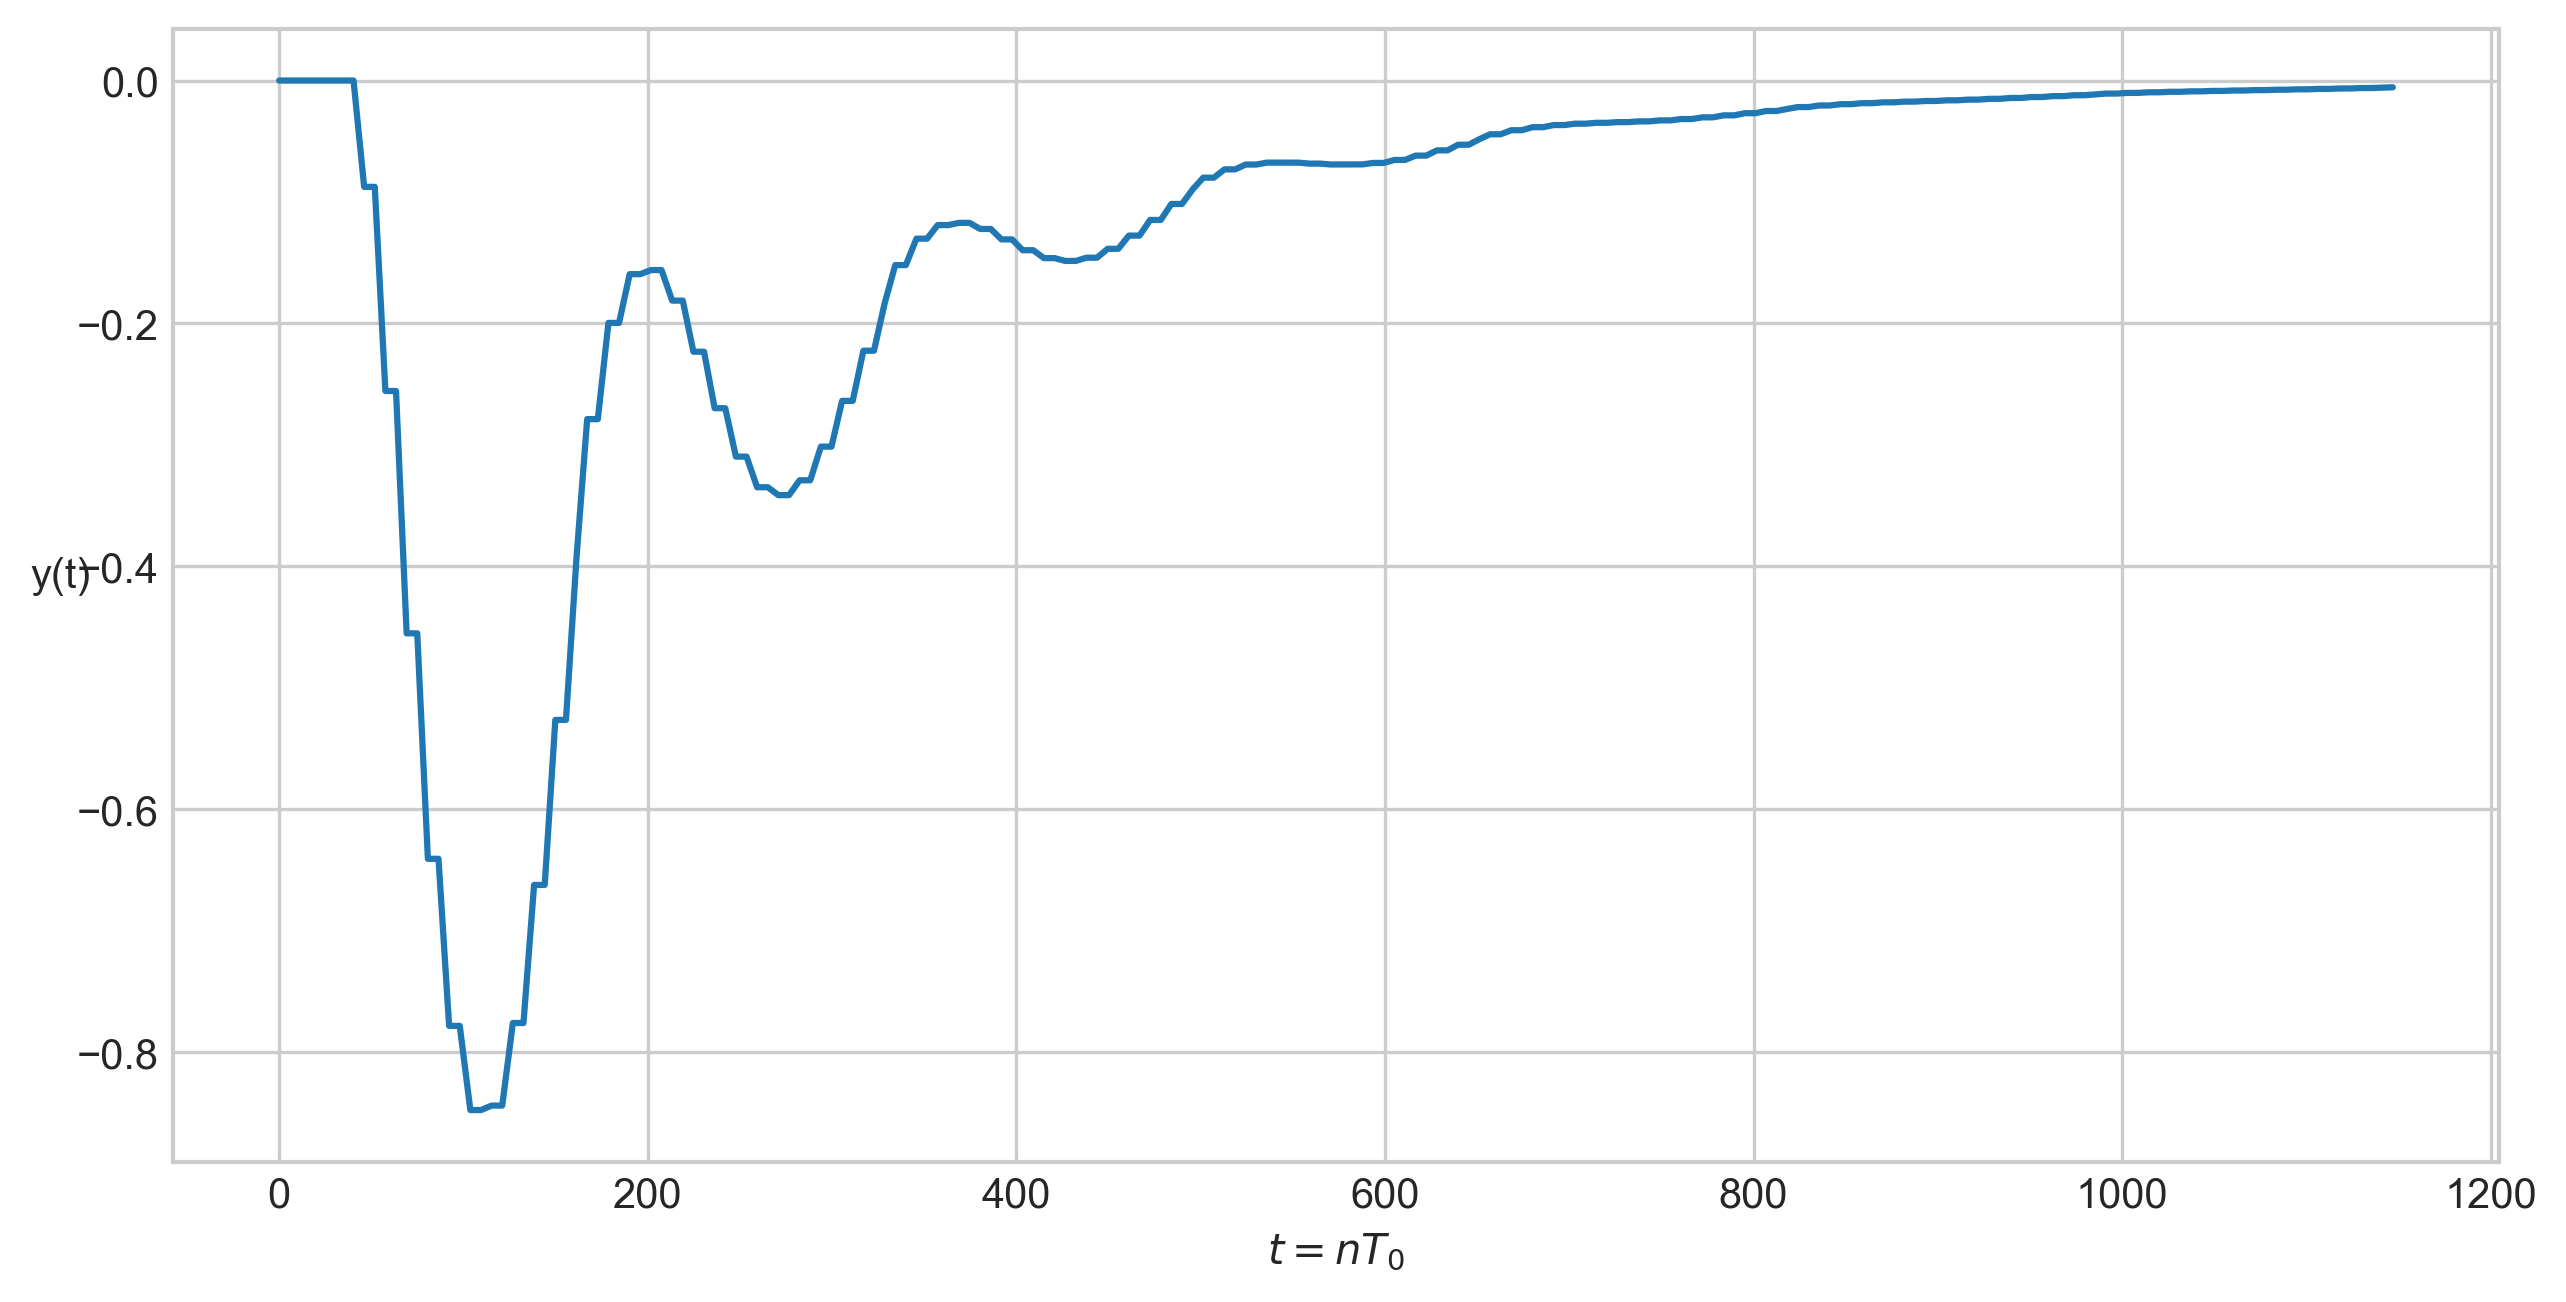
\includegraphics[width=\textwidth]{pics/transient_process_final_9_1_impulse.png}
\end{center}
% Перехідний процес при подачі на задаюче діяння одиничного ступінчатого збурення:
% \begin{center}
%     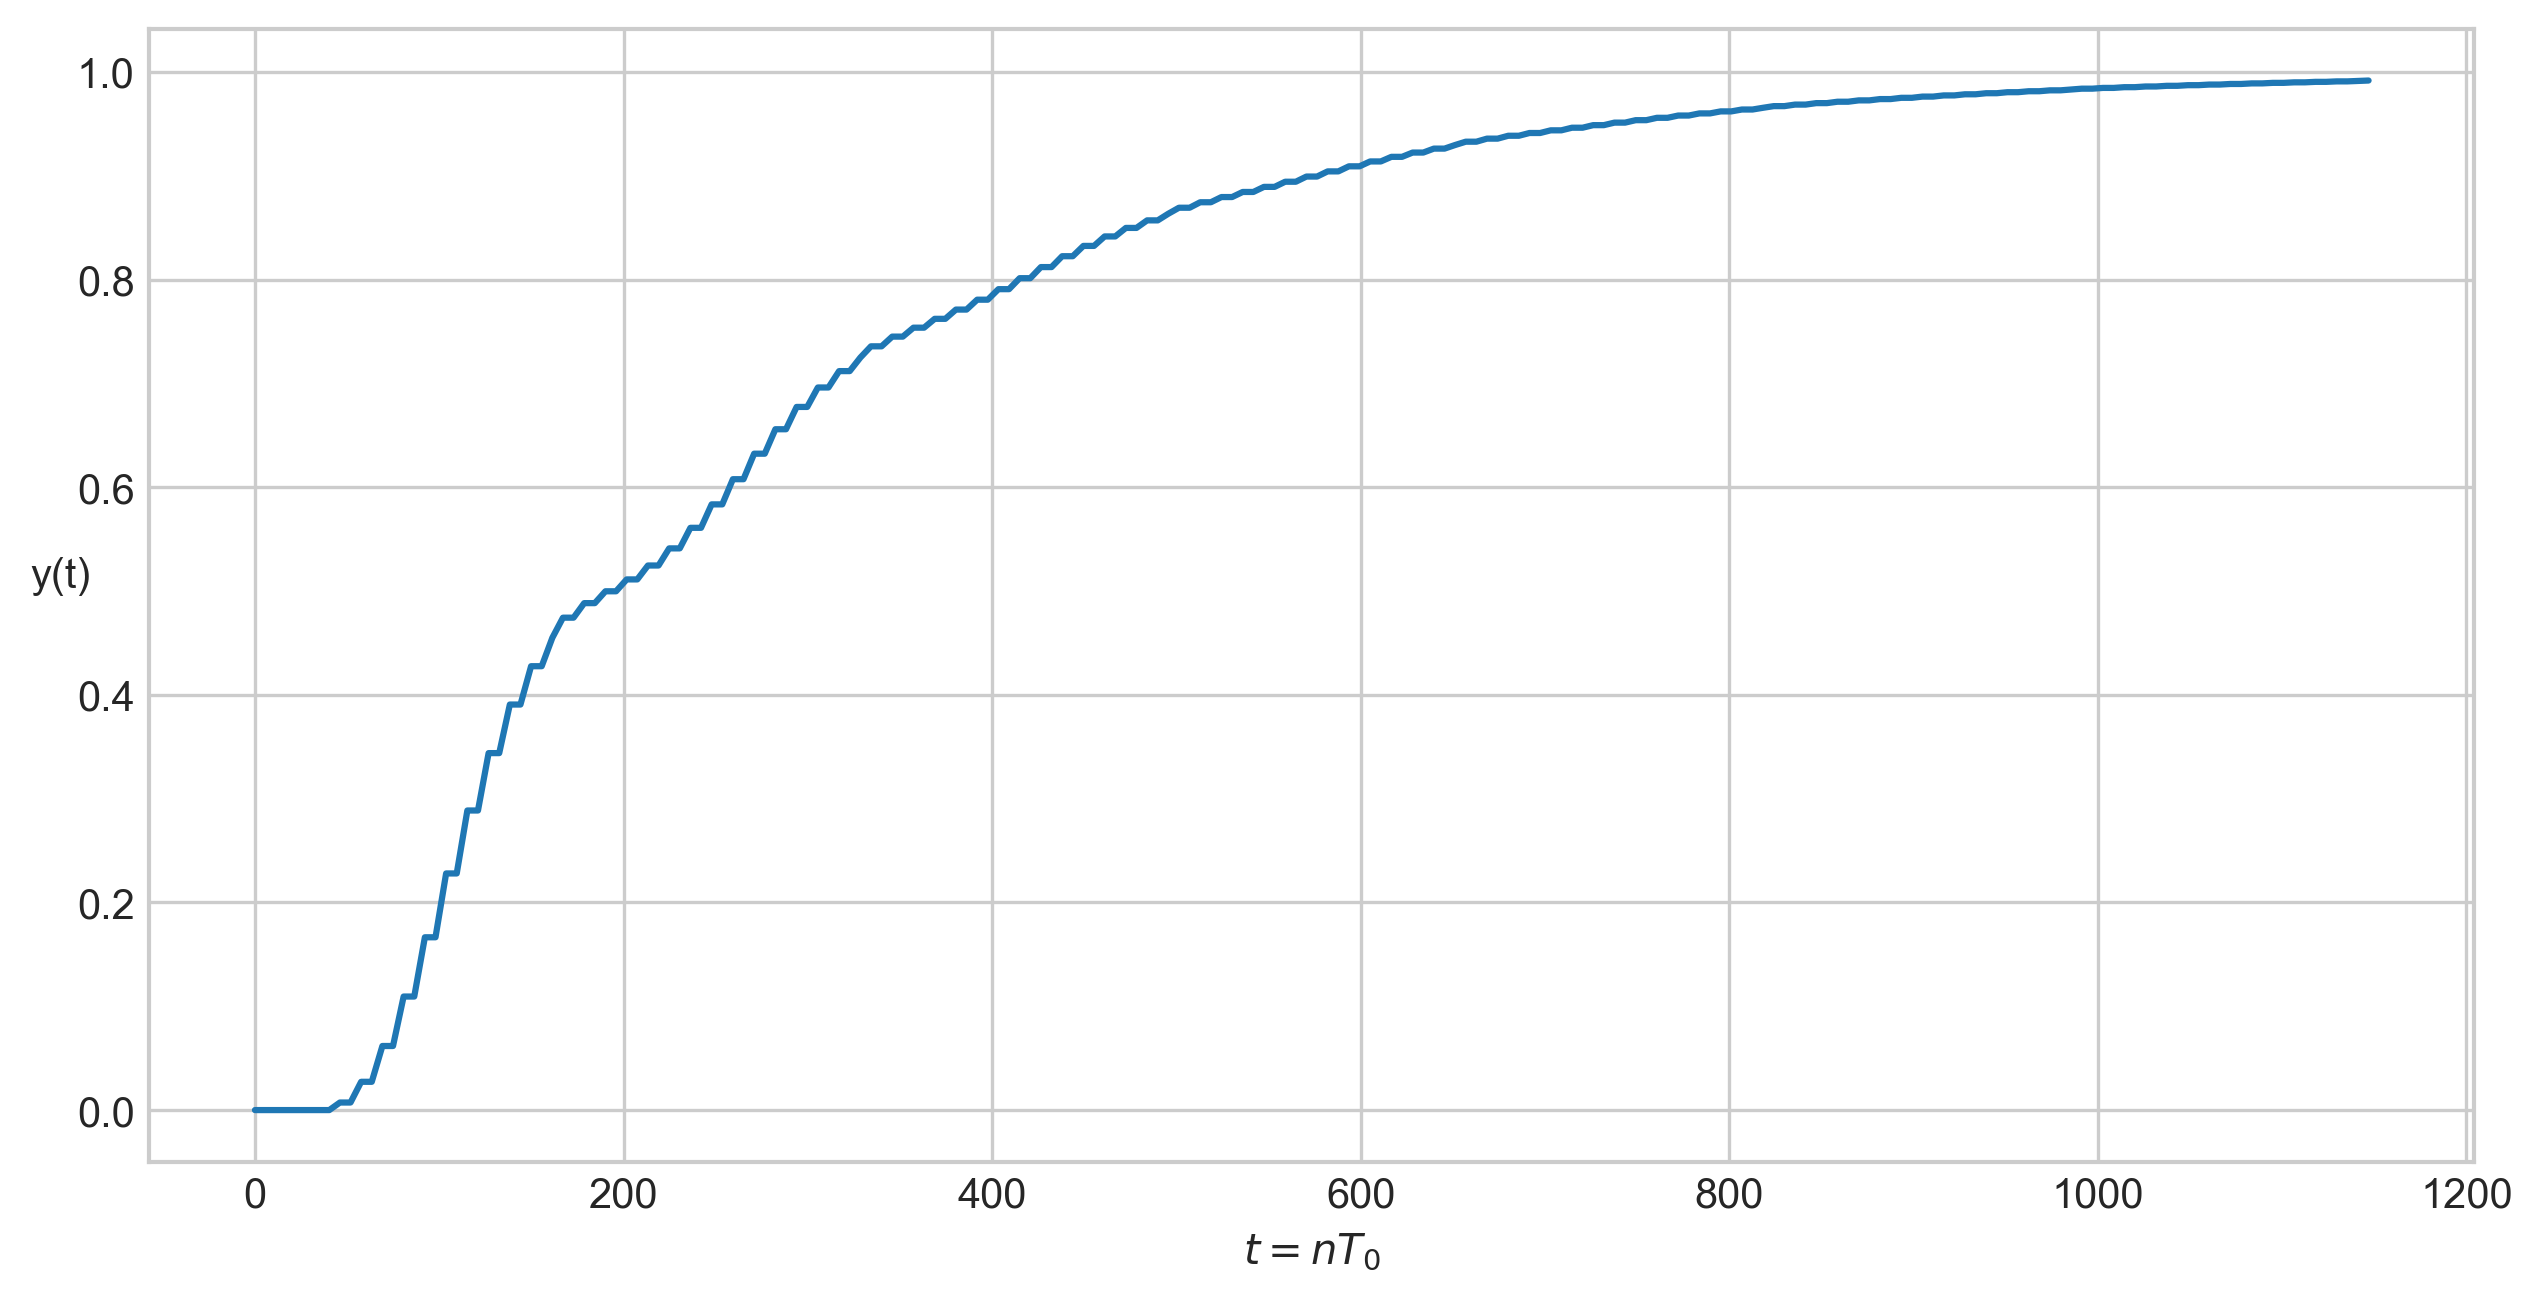
\includegraphics[scale=0.7]{pics/transient_process_final_9_1_step.png}
% \end{center}

\section{Випадок 
\texorpdfstring{$W_O(s) = \frac{ k e^{-\tau s}}{(T_1 s + 1) (T_2 s + 1)}$}{1}}
Оптимальні настройки регулятора було обчислено в пункті \ref{sec:resonance_2nd_order}.
Зв'язок між вихідною координатою та керуючим діянням задається диференціальним рівнянням
\begin{gather*}
    \mbox{\normalsize 
    $T_1 T_2 \frac{d^2 y(t)}{dt^2} +
    \left(T_1 + T_2 \right) \frac{d y(t)}{dt} + y(t) = k u(t-\tau)$}
\end{gather*}
Перехідний процес при подачі на задаюче діяння одиничного імпульсу:
\begin{center}
    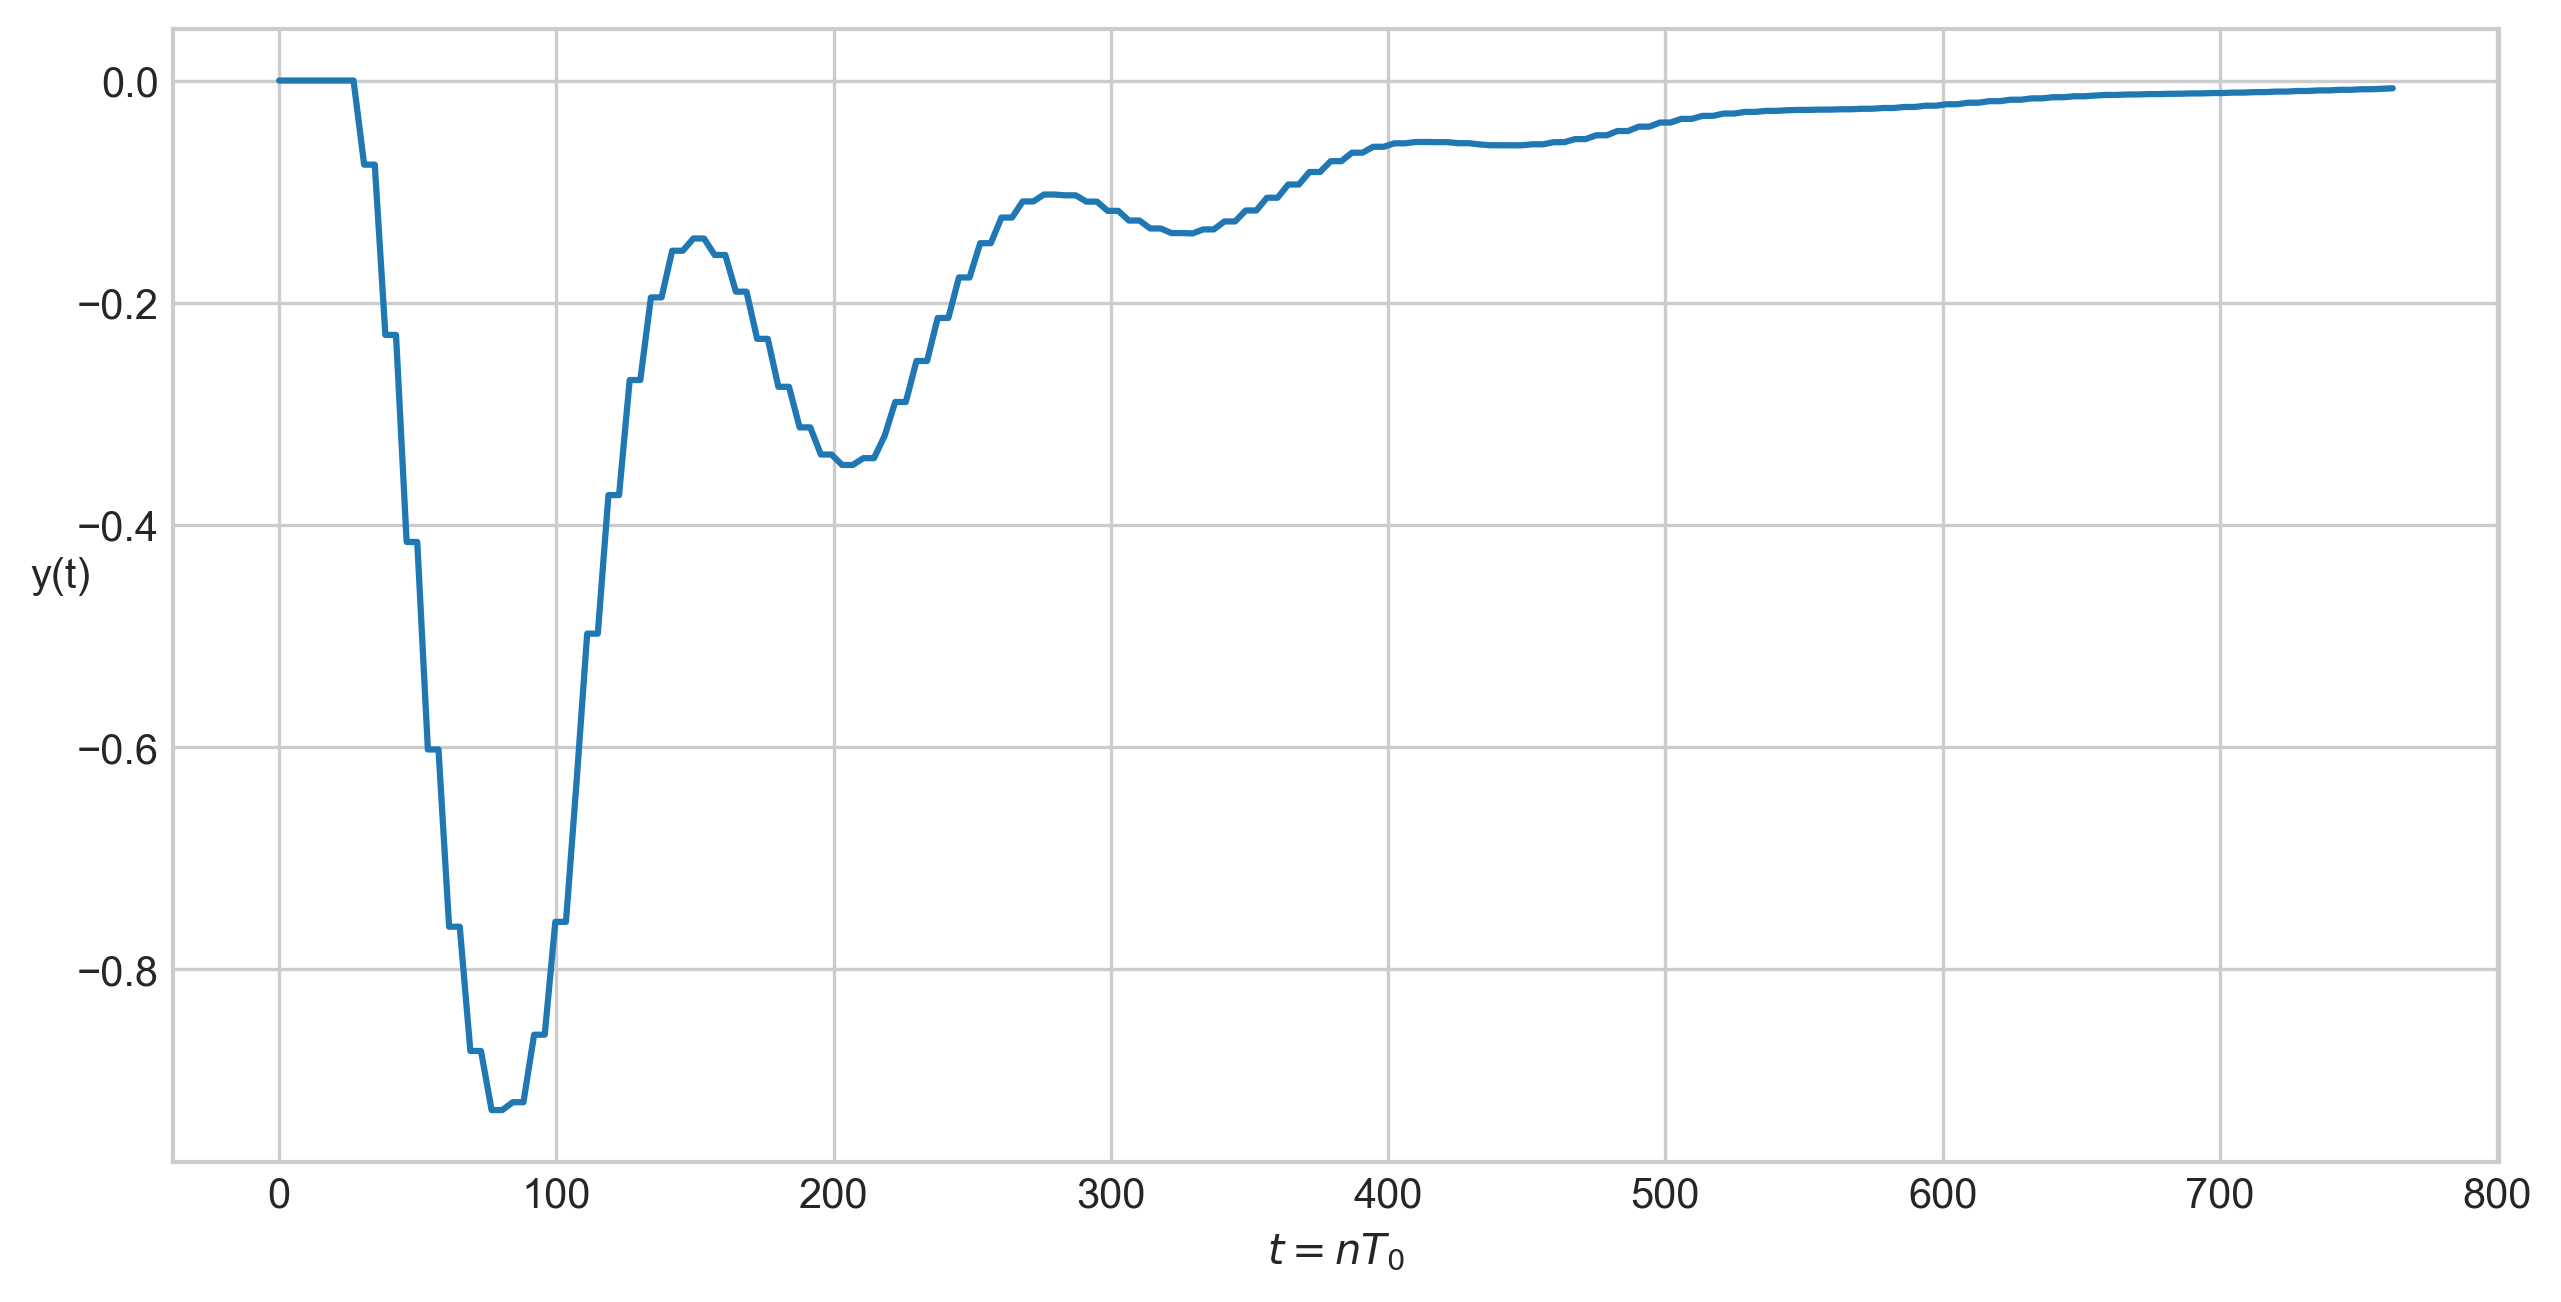
\includegraphics[width=\textwidth]{pics/transient_process_final_9_2_impulse.png}
\end{center}
% Перехідний процес при подачі на задаюче діяння одиничного ступінчатого збурення:
% \begin{center}
%     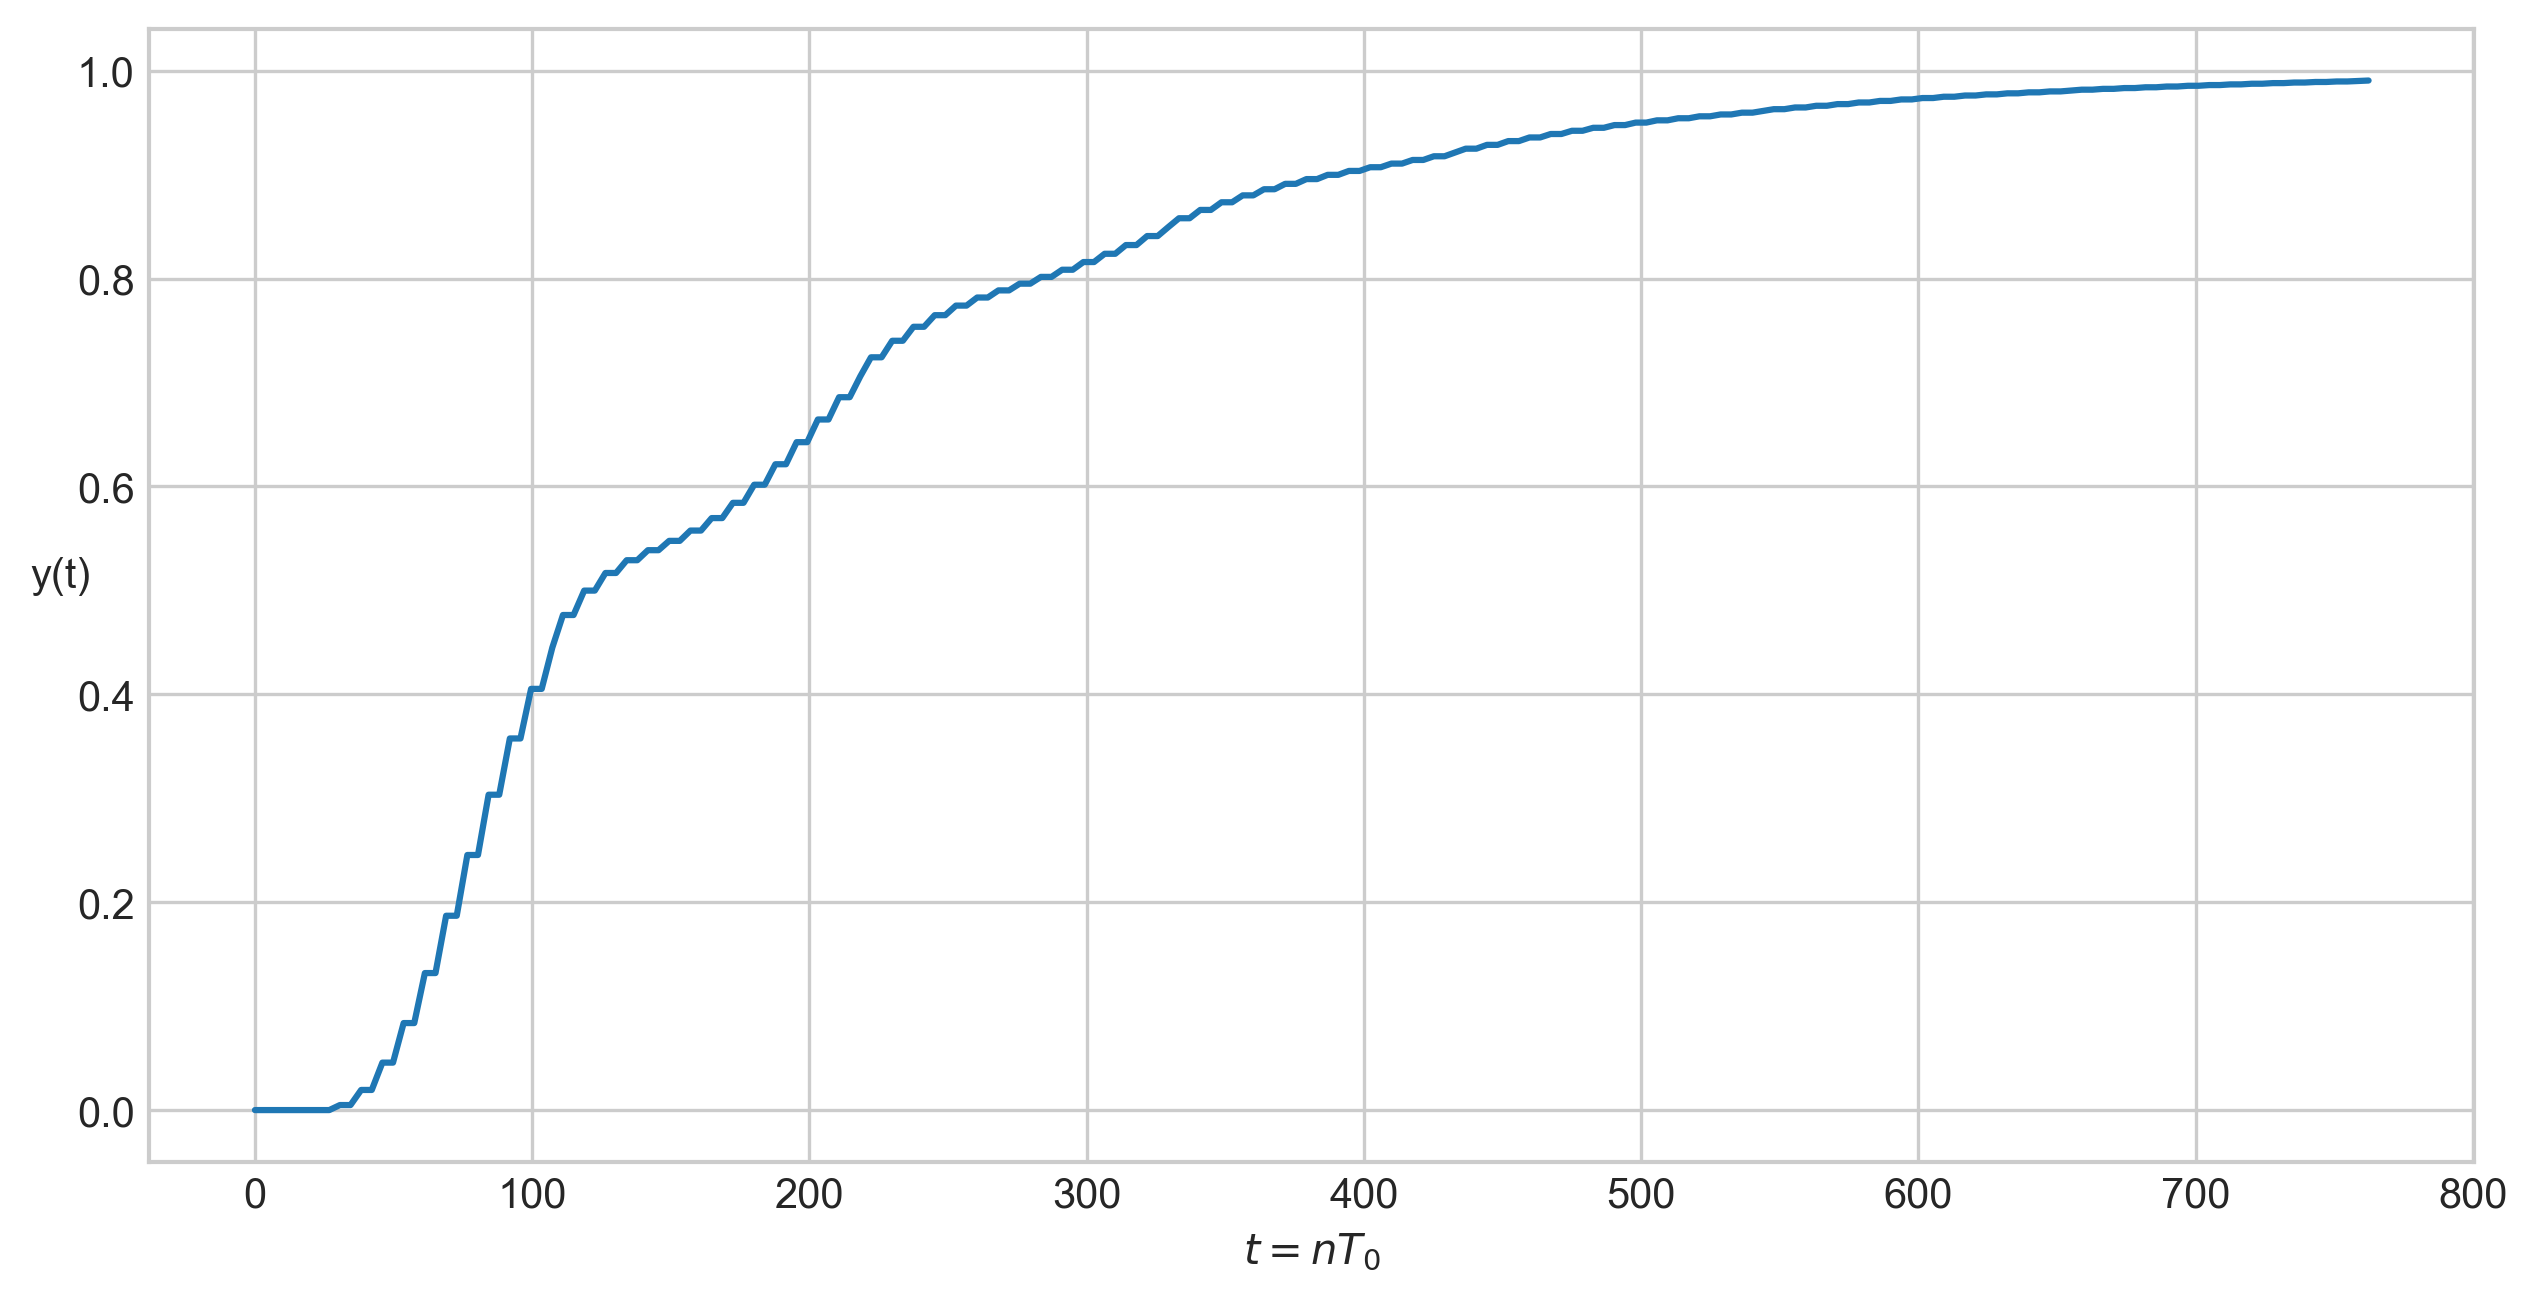
\includegraphics[scale=0.7]{pics/transient_process_final_9_2_step.png}
% \end{center}

\section{Випадок 
\texorpdfstring{$W_O(s) = \frac{ k e^{-\tau s}}{T_1 s + 1}$}{1}}
Оптимальні настройки регулятора для різних значень параметра $\lambda$ 
було обчислено в розділі \ref{ch:direct}.
Зв'язок між вихідною координатою та керуючим діянням задається диференціальним рівнянням
\begin{gather*}
    \mbox{\normalsize 
    $T_1 \frac{d y(t)}{dt} + y(t) = k u(t-\tau)$
    }
\end{gather*}
% Перехідні процеси при подачі на задаюче діяння одиничного імпульсу:
% \begin{center}
%     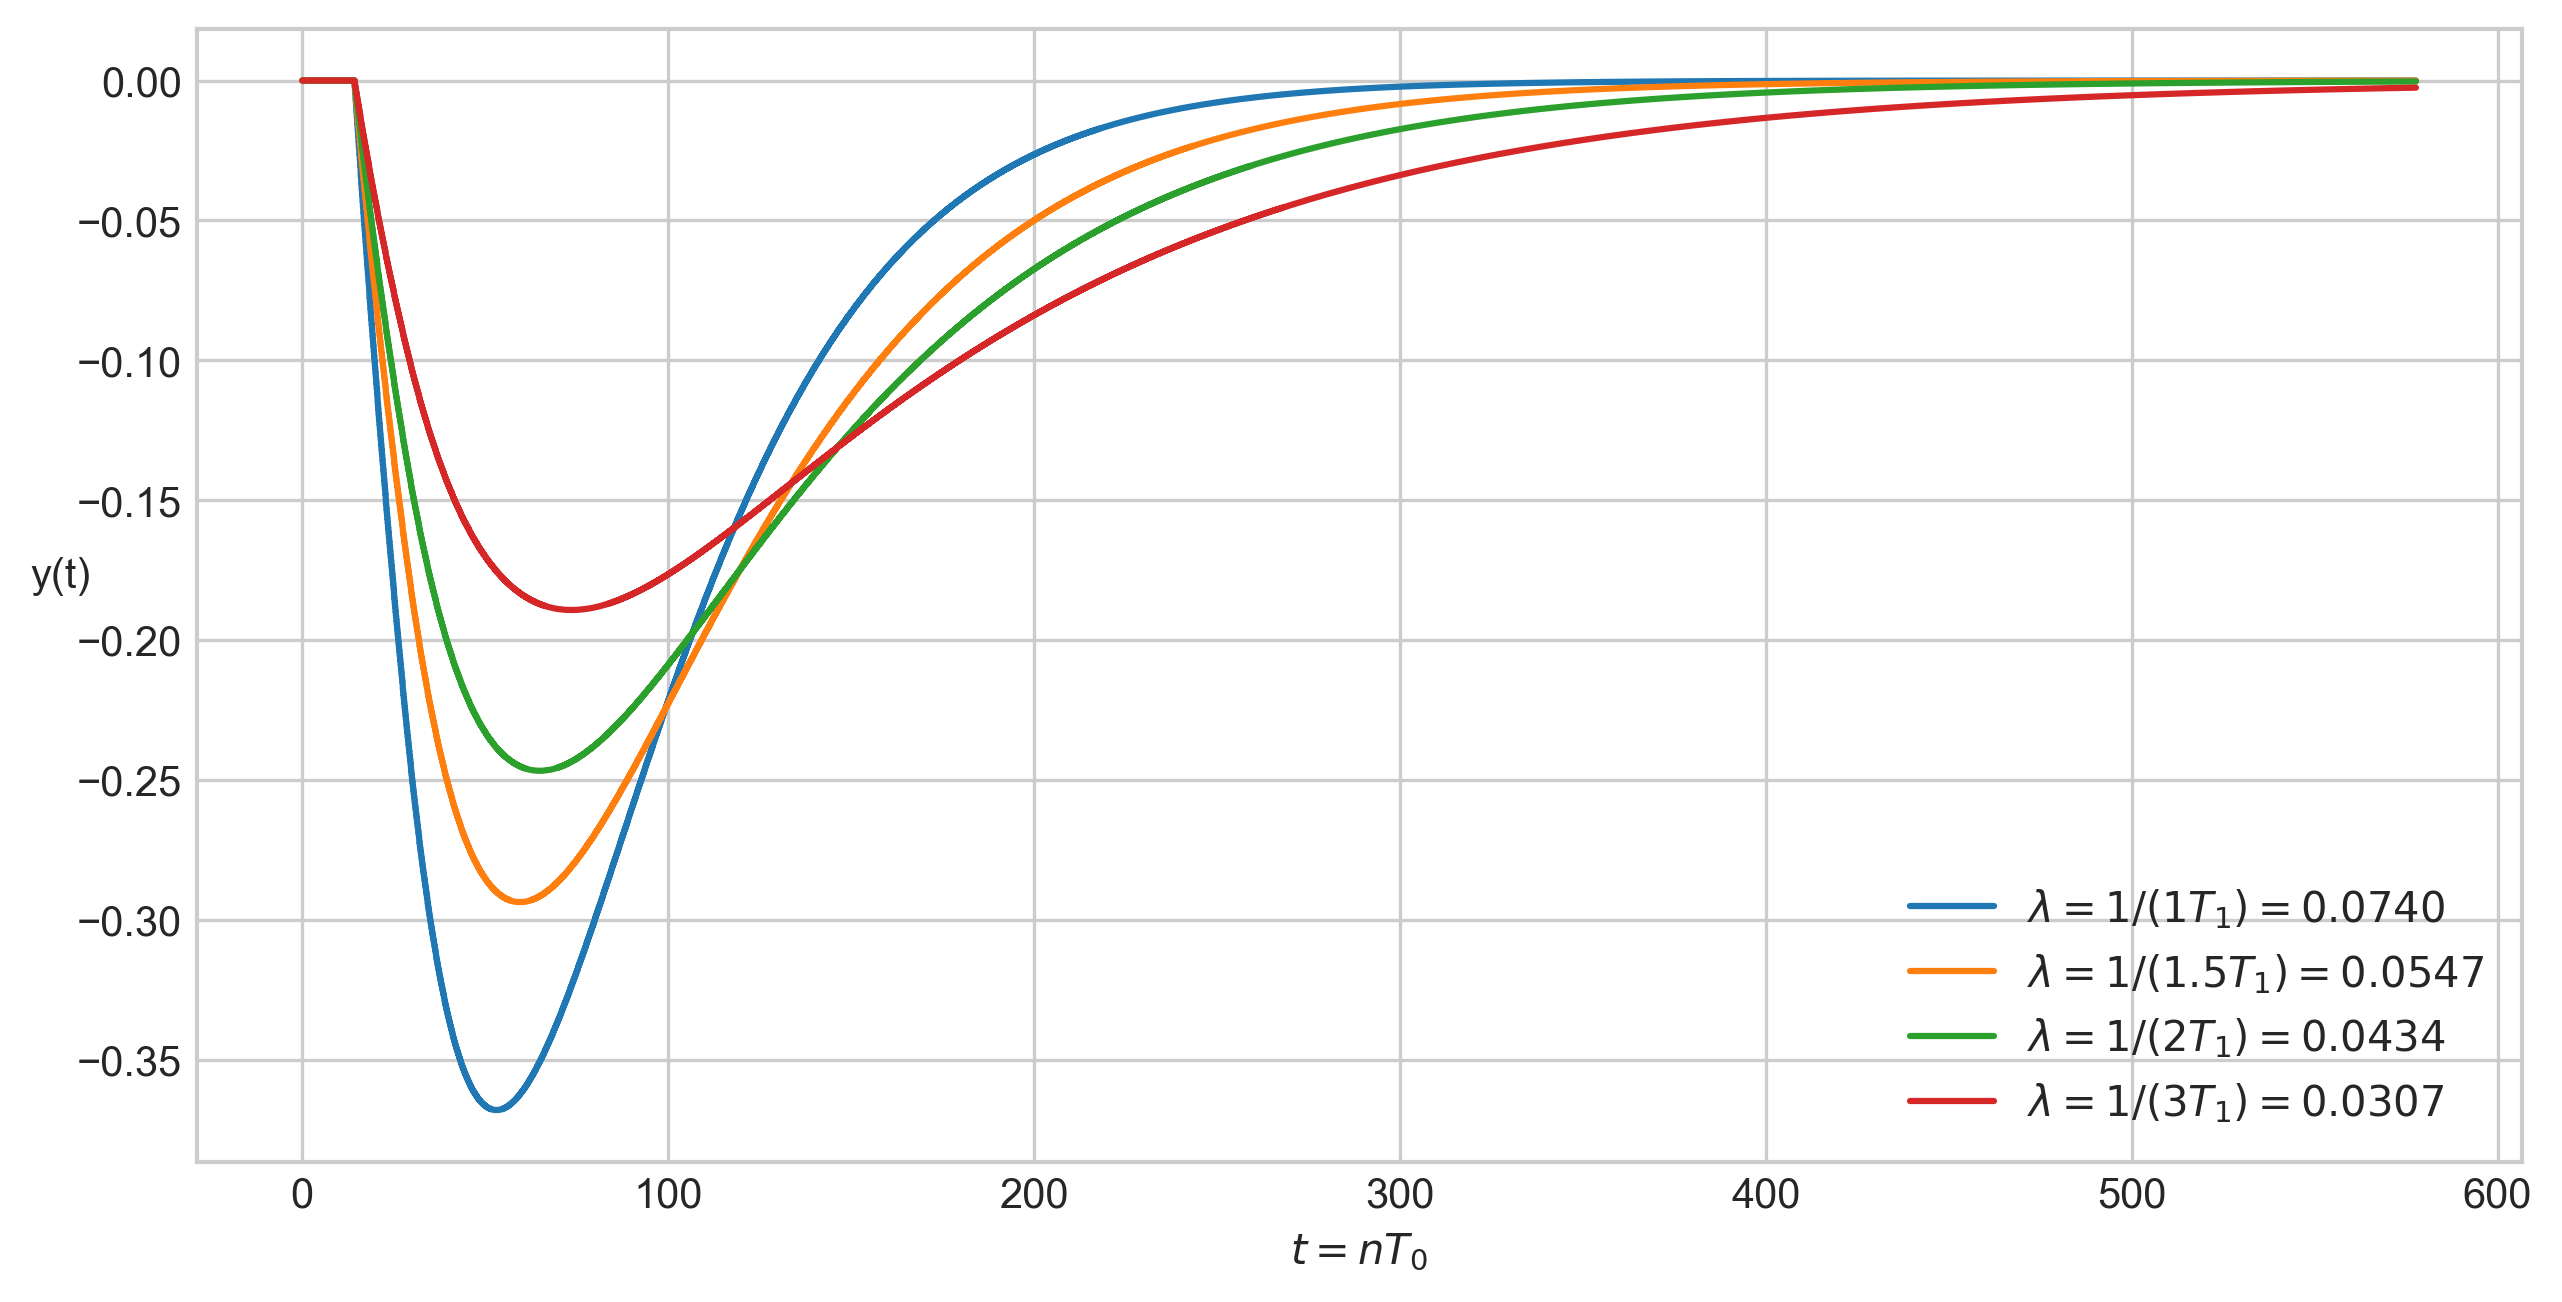
\includegraphics[scale=0.7]{pics/transient_process_final_9_3_impulse.png}
% \end{center}
Перехідні процеси при подачі на задаюче діяння одиничного ступінчатого збурення:
\begin{center}
    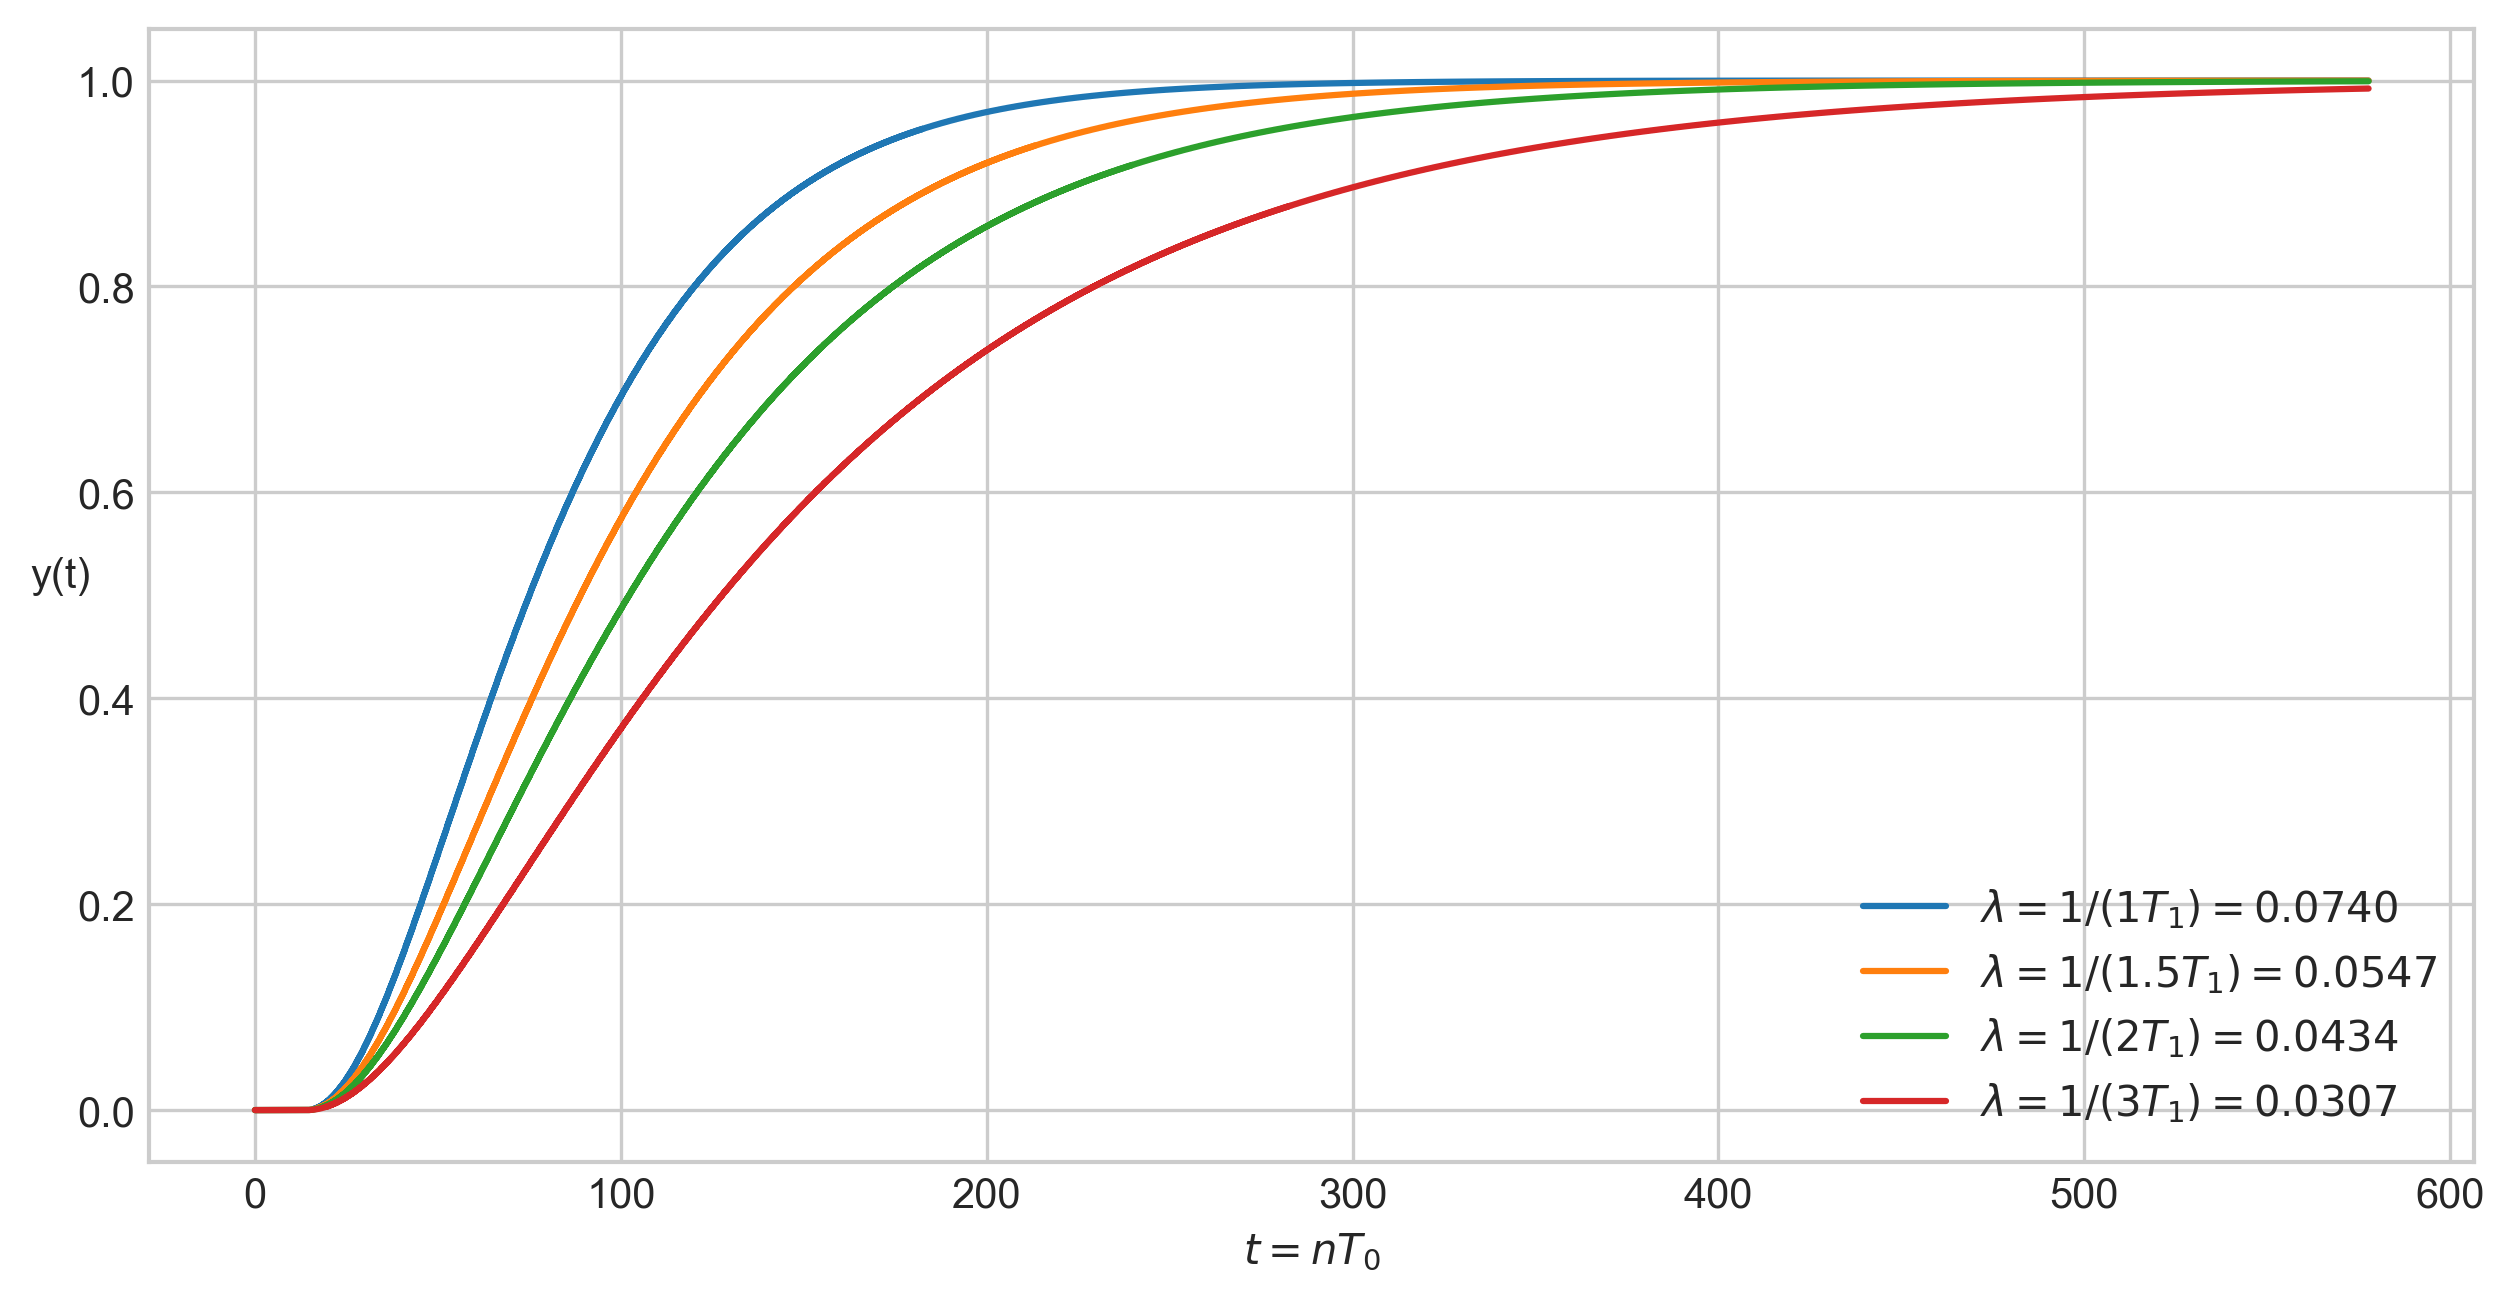
\includegraphics[width=\textwidth]{pics/transient_process_final_9_3_step.png}
\end{center}
    \newpage

    \bibsection
    \begin{enumerate}
        \item Конспект лекцій з теорії керування, Романенко В.Д.
        \item Теорія керування: методичні рекомендації для курсового проектування для 
        студентів напряму підготовки 6.040303 –-- системний аналіз / Укладач: В. Д. Романенко. ---
        К.: ННК <<ІПСА>> НТУУ <<КПІ>>, 2012. --- 43 с.
    \end{enumerate}
\end{document}